% Options for packages loaded elsewhere
\PassOptionsToPackage{unicode}{hyperref}
\PassOptionsToPackage{hyphens}{url}
\PassOptionsToPackage{dvipsnames,svgnames,x11names}{xcolor}
%
\documentclass[
  letterpaper,
  DIV=11,
  numbers=noendperiod]{scrartcl}

\usepackage{amsmath,amssymb}
\usepackage{iftex}
\ifPDFTeX
  \usepackage[T1]{fontenc}
  \usepackage[utf8]{inputenc}
  \usepackage{textcomp} % provide euro and other symbols
\else % if luatex or xetex
  \usepackage{unicode-math}
  \defaultfontfeatures{Scale=MatchLowercase}
  \defaultfontfeatures[\rmfamily]{Ligatures=TeX,Scale=1}
\fi
\usepackage{lmodern}
\ifPDFTeX\else  
    % xetex/luatex font selection
\fi
% Use upquote if available, for straight quotes in verbatim environments
\IfFileExists{upquote.sty}{\usepackage{upquote}}{}
\IfFileExists{microtype.sty}{% use microtype if available
  \usepackage[]{microtype}
  \UseMicrotypeSet[protrusion]{basicmath} % disable protrusion for tt fonts
}{}
\makeatletter
\@ifundefined{KOMAClassName}{% if non-KOMA class
  \IfFileExists{parskip.sty}{%
    \usepackage{parskip}
  }{% else
    \setlength{\parindent}{0pt}
    \setlength{\parskip}{6pt plus 2pt minus 1pt}}
}{% if KOMA class
  \KOMAoptions{parskip=half}}
\makeatother
\usepackage{xcolor}
\usepackage[right=1in,left=1in]{geometry}
\setlength{\emergencystretch}{3em} % prevent overfull lines
\setcounter{secnumdepth}{5}
% Make \paragraph and \subparagraph free-standing
\ifx\paragraph\undefined\else
  \let\oldparagraph\paragraph
  \renewcommand{\paragraph}[1]{\oldparagraph{#1}\mbox{}}
\fi
\ifx\subparagraph\undefined\else
  \let\oldsubparagraph\subparagraph
  \renewcommand{\subparagraph}[1]{\oldsubparagraph{#1}\mbox{}}
\fi


\providecommand{\tightlist}{%
  \setlength{\itemsep}{0pt}\setlength{\parskip}{0pt}}\usepackage{longtable,booktabs,array}
\usepackage{calc} % for calculating minipage widths
% Correct order of tables after \paragraph or \subparagraph
\usepackage{etoolbox}
\makeatletter
\patchcmd\longtable{\par}{\if@noskipsec\mbox{}\fi\par}{}{}
\makeatother
% Allow footnotes in longtable head/foot
\IfFileExists{footnotehyper.sty}{\usepackage{footnotehyper}}{\usepackage{footnote}}
\makesavenoteenv{longtable}
\usepackage{graphicx}
\makeatletter
\def\maxwidth{\ifdim\Gin@nat@width>\linewidth\linewidth\else\Gin@nat@width\fi}
\def\maxheight{\ifdim\Gin@nat@height>\textheight\textheight\else\Gin@nat@height\fi}
\makeatother
% Scale images if necessary, so that they will not overflow the page
% margins by default, and it is still possible to overwrite the defaults
% using explicit options in \includegraphics[width, height, ...]{}
\setkeys{Gin}{width=\maxwidth,height=\maxheight,keepaspectratio}
% Set default figure placement to htbp
\makeatletter
\def\fps@figure{htbp}
\makeatother
\newlength{\cslhangindent}
\setlength{\cslhangindent}{1.5em}
\newlength{\csllabelwidth}
\setlength{\csllabelwidth}{3em}
\newlength{\cslentryspacingunit} % times entry-spacing
\setlength{\cslentryspacingunit}{\parskip}
\newenvironment{CSLReferences}[2] % #1 hanging-ident, #2 entry spacing
 {% don't indent paragraphs
  \setlength{\parindent}{0pt}
  % turn on hanging indent if param 1 is 1
  \ifodd #1
  \let\oldpar\par
  \def\par{\hangindent=\cslhangindent\oldpar}
  \fi
  % set entry spacing
  \setlength{\parskip}{#2\cslentryspacingunit}
 }%
 {}
\usepackage{calc}
\newcommand{\CSLBlock}[1]{#1\hfill\break}
\newcommand{\CSLLeftMargin}[1]{\parbox[t]{\csllabelwidth}{#1}}
\newcommand{\CSLRightInline}[1]{\parbox[t]{\linewidth - \csllabelwidth}{#1}\break}
\newcommand{\CSLIndent}[1]{\hspace{\cslhangindent}#1}

\usepackage{booktabs}
\usepackage{longtable}
\usepackage{array}
\usepackage{multirow}
\usepackage{wrapfig}
\usepackage{float}
\usepackage{colortbl}
\usepackage{pdflscape}
\usepackage{tabu}
\usepackage{threeparttable}
\usepackage{threeparttablex}
\usepackage[normalem]{ulem}
\usepackage{makecell}
\usepackage{xcolor}
\usepackage{colortbl}
\makeatletter
\renewenvironment{table}%
  {\renewcommand\familydefault\sfdefault
   \@float{table}}
  {\end@float}
\makeatother
\KOMAoption{captions}{tableheading}
\makeatletter
\makeatother
\makeatletter
\makeatother
\makeatletter
\@ifpackageloaded{caption}{}{\usepackage{caption}}
\AtBeginDocument{%
\ifdefined\contentsname
  \renewcommand*\contentsname{Table of contents}
\else
  \newcommand\contentsname{Table of contents}
\fi
\ifdefined\listfigurename
  \renewcommand*\listfigurename{List of Figures}
\else
  \newcommand\listfigurename{List of Figures}
\fi
\ifdefined\listtablename
  \renewcommand*\listtablename{List of Tables}
\else
  \newcommand\listtablename{List of Tables}
\fi
\ifdefined\figurename
  \renewcommand*\figurename{Figure}
\else
  \newcommand\figurename{Figure}
\fi
\ifdefined\tablename
  \renewcommand*\tablename{Table}
\else
  \newcommand\tablename{Table}
\fi
}
\@ifpackageloaded{float}{}{\usepackage{float}}
\floatstyle{ruled}
\@ifundefined{c@chapter}{\newfloat{codelisting}{h}{lop}}{\newfloat{codelisting}{h}{lop}[chapter]}
\floatname{codelisting}{Listing}
\newcommand*\listoflistings{\listof{codelisting}{List of Listings}}
\makeatother
\makeatletter
\@ifpackageloaded{caption}{}{\usepackage{caption}}
\@ifpackageloaded{subcaption}{}{\usepackage{subcaption}}
\makeatother
\makeatletter
\@ifpackageloaded{tcolorbox}{}{\usepackage[skins,breakable]{tcolorbox}}
\makeatother
\makeatletter
\@ifundefined{shadecolor}{\definecolor{shadecolor}{rgb}{.97, .97, .97}}
\makeatother
\makeatletter
\makeatother
\makeatletter
\makeatother
\ifLuaTeX
  \usepackage{selnolig}  % disable illegal ligatures
\fi
\IfFileExists{bookmark.sty}{\usepackage{bookmark}}{\usepackage{hyperref}}
\IfFileExists{xurl.sty}{\usepackage{xurl}}{} % add URL line breaks if available
\urlstyle{same} % disable monospaced font for URLs
\hypersetup{
  pdftitle={How Do Household Energy Transitions Work?},
  pdfauthor={Jill Baumgartner (Co-PI); Sam Harper (Co-PI); On behalf of the Beijing Household Energy Transitions Team},
  colorlinks=true,
  linkcolor={blue},
  filecolor={Maroon},
  citecolor={Blue},
  urlcolor={Blue},
  pdfcreator={LaTeX via pandoc}}

\title{How Do Household Energy Transitions Work?}
\author{Jill Baumgartner (Co-PI) \and Sam Harper (Co-PI) \and On behalf
of the Beijing Household Energy Transitions Team}
\date{2024-04-18}

\begin{document}
\maketitle
\ifdefined\Shaded\renewenvironment{Shaded}{\begin{tcolorbox}[boxrule=0pt, sharp corners, breakable, borderline west={3pt}{0pt}{shadecolor}, interior hidden, frame hidden, enhanced]}{\end{tcolorbox}}\fi

\renewcommand*\contentsname{Table of contents}
{
\hypersetup{linkcolor=}
\setcounter{tocdepth}{3}
\tableofcontents
}
\hypertarget{abstract}{%
\subsection*{Abstract}\label{abstract}}

\hypertarget{introduction}{%
\subsubsection*{Introduction}\label{introduction}}

\hypertarget{methods}{%
\subsubsection*{Methods}\label{methods}}

\hypertarget{results}{%
\subsubsection*{Results}\label{results}}

\hypertarget{conclusions}{%
\subsubsection*{Conclusions}\label{conclusions}}

\hypertarget{introductiona}{%
\section{Introduction{[}a{]}}\label{introductiona}}

China is deploying an ambitious policy to transition up to 70\% of
households in northern China to clean space heating, including a
large-scale roll out across rural and peri-urban Beijing, referred to in
this document as the China's Coal Ban and Heat Pump (CBHP) subsidy
policy. To meet this target the Beijing municipal government announced a
two-pronged program that designates coal-restricted areas and
simultaneously offers subsidies to night-time electricity rates and for
the purchase and installation of electric-powered, air-source heat pumps
to replace traditional coal-heating stoves. The policy was piloted in
2015 and, starting in 2016, was rolled out on a village-by-village
basis; however there is uncertainty as to when villages will receive the
program. The variability in when the policy is applied to each village
allows us to treat the roll-out of the program as a quasi-randomized
intervention. Households may also be differentially affected by this
program due to factors such as financial constraints, preferences and
social capital, and there is uncertainty about whether and how this
intervention may affect indoor and outdoor air pollution, as well as
heating behaviors and health outcomes.

\hypertarget{background}{%
\section{Background}\label{background}}

\hypertarget{context-for-the-policy}{%
\subsection{Context for the policy}\label{context-for-the-policy}}

Beijing has a temperate continental monsoon climate characterized by
cold, dry winters and hot, humid summers. Access to central heating is
limited to urban areas and households in most rural and peri-urban areas
of Beijing historically heated their homes using mostly coal heaters and
biomass-fueled \emph{kangs} (a traditional Chinese energy technology
that integrates at least four different home functions including
cooking, a bed for sleeping, space heating, and home ventilation).
Household coal burning was a major contributor to indoor and outdoor air
pollution in northern China, especially in winter. In 2015, over 100
million rural households consumed around 200 million tons of coal to
meet over 80\% of northern China's residential space heating demand
(Dispersed Coal Management Research Group 2023). At that time, household
coal-fuelled heaters burned approximately half of the over 400 million
tons of coal used for space heating (Group 2016) and contributed to
\textasciitilde30\% of northern China's wintertime air pollution. In
2013, exposure to ambient fine particulate matter from coal combustion -
from industry, electricity, and domestic sources - was the largest
estimated contributor to population exposure to PM\textsubscript{2.5}
and contributed to an estimated 366,000 premature deaths annually in
China (Group 2016).

Replacing household coal stoves with clean heating alternatives was
considered a potentially impactful intervention to improve rural
development, reduce PM\textsubscript{2.5} across the region, and
mitigate air pollution-related health impacts. A number of clean heating
options including electric heat pumps, gas heaters, pelletized biomass
stoves, and electric resistance heaters with thermal storage were widely
promoted by the Chinese government (Dispersed Coal Management Research
Group 2023). By 2021, over 36 million households in northern China were
treated by the policy and an estimated 21 million additional households
are expected to be treated by 2025. Whether this large-scale energy
policy yielded air quality and health benefits remains a critical and
unresolved question.

\hypertarget{prior-evidence-on-household-energy-interventions-and-air-pollution}{%
\subsection{Prior evidence on household energy interventions and air
pollution}\label{prior-evidence-on-household-energy-interventions-and-air-pollution}}

Household energy interventions, mostly cooking-related, that replace
solid fuel stoves with cleaner-burning alternatives have been
implemented and studied extensively in countries including China over
the past several decades. While their introduction of more efficient
residential stoves and fuels is expected to reduce air pollution
emissions and subsequent exposures, there is still no consensus about
their effectiveness in achieving health-relevant air pollution
reductions in real-world settings (Quansah et al. 2017). In particular,
the effectiveness of large-scale household energy programs like China's
Coal Ban and Heat Pump (CBHP) subsidy have been rarely empirically
investigated, especially at sub-city spatial resolution. In Ireland,
county-level residential coal bans in the 1990s were associated with
40-70\% decreases in black smoke concentrations in ban-affected areas
(Dockery et al. 2013). In Australia, a wood-burning stove exchange lower
daily wintertime PM\textsubscript{10} from 44 to 27 µg/m3 (Johnston et
al. 2013), and clean energy policies in New Zealand were associated with
11-36\% reductions in winter PM\textsubscript{10} (Scott and Scarrott
2011). The few evaluations of the CBHP policy observed small decreases
in outdoor PM\textsubscript{2.5} (-7 to -2.4 µg/m\textsuperscript{3}) in
municipalities or prefectures in the policy compared with neighboring
areas not affected by the policy (Niu et al. 2024; Song et al. 2023; Tan
et al. 2023; Yu et al. 2021), and a recent modeling study estimated 36\%
lower personal exposure to PM\textsubscript{2.5} based on
household-reported changes in fuel use (Meng et al. 2023). However, none
of these studies included field-based measurements of air pollution or
personal exposures, which are known to differ considerably from modeled
estimates (Thompson et al. 2019), and few accounted for secular changes
in air quality over time, limiting any conclusions about the air quality
benefits of the CBHP policy.

\hypertarget{prior-evidence-on-clean-energy-interventions-and-cardiovascular-outcomes}{%
\subsection{Prior evidence on clean energy interventions and
cardiovascular
outcomes}\label{prior-evidence-on-clean-energy-interventions-and-cardiovascular-outcomes}}

Most previous health assessments of household energy interventions have
focused on cookstoves instead of heating. Published results from
randomized trials of less polluting cookstoves generally indicate a
cardiovascular benefit. In older Guatemalan women, a chimney stove
intervention lowered exposure to air pollution and reduced the
occurrence of nonspecific ST-segment depression (McCracken et al. 2011).
That same study in Guatemala and randomized trials in Nigeria and Ghana
also observed reductions in blood pressure (systolic range: −3.7 to −1.3
mmHg) in women assigned to gas, ethanol, or improved combustion biomass
stoves, and are supported by non-randomized, controlled (pre-post
design) intervention studies in Nicaragua and Bolivia showing even
larger SBP reductions (−5.9 and −5.5 mmHg, respectively) (Onakomaiya et
al. 2019). In contrast, a recent multi-country randomized trial did not
observe a protective effect of gas stoves on gestational blood pressure
(Ye et al. 2022) despite large reductions (\textasciitilde66\% lower) in
exposure to PM\textsubscript{2.5}(Johnson et al. 2022).

The few population-based evaluations of large-scale residential energy
policies also suggest a cardio-respiratory benefit of clean energy
transition. Residential wood-burning bans were associated with
reductions in cardiovascular hospitalizations (-7\%) in California (Yap
and Garcia 2015) and with reduced cardiovascular (-17.9\%) and
respiratory (−22.8\%) mortality in Australia (Johnston et al. 2013),
though neither study fully controlled for possible secular improvements
in health. Most relevant to our study are two quasi-experimental
assessments of coal replacement policies. In Ireland, reductions in
respiratory not but cardiovascular mortality were observed following a
coal ban (Dockery et al. 2013). A multi-city study of Chinese adults in
cities where the CBHP was piloted compared with adults in cities not in
the pilot observed small decreases in chronic lung diseases (-3.0 to
-1.1\%) but no change in physician-diagnosed cardiovascular diseases,
potentially due to the short (one-year) post-policy evaluation period or
confounding by other unmeasured city-wide air quality or health-related
policies (Wen et al. 2023).

Though{[}b{]} household air pollution is a well-established health risk
factor, which energy interventions can reduce air pollution exposures,
improve health, and are scalable and sustainable remains a critical and
unanswered question. In a recent Official American Thoracic Society
Statement, for example, the committee could not reach a consensus on
whether previously studied household energy interventions (including
gas, ethanol, solar, and improved biomass stoves) improved health
outcomes that included blood pressure (with 55\% saying no and 45\%
saying yes) (Harrison et al. Approved February 2024).

\hypertarget{assessing-dynamic-and-heterogeneous-treatment-effects}{%
\subsection{Assessing dynamic and heterogeneous treatment
effects}\label{assessing-dynamic-and-heterogeneous-treatment-effects}}

Since 2015, thousands of villages across Beijing and northern China
entered the CBHP policy prior to the start of the heating season each
year. Given the many behavioral, social, or economic factors that might
affect both new heater use and coal stove suspension (e.g., energy
prices and availability, wintertime temperature, COVID-19 pandemic, user
preferences), it is possible that the effect of the policy on air
pollution and health may be dynamic over time and/or heterogeneous
across treatment cohorts. Thus, it may be important to study both the
overall and group-time effects of the policy.

\hypertarget{evaluating-the-mechanisms-through-which-policies-may-affect-health-outcomes.}{%
\subsection{Evaluating the mechanisms through which policies may affect
health
outcomes.}\label{evaluating-the-mechanisms-through-which-policies-may-affect-health-outcomes.}}

With several exceptions (Alexander et al. 2018; Gould et al. 2023;
McCracken et al. 2007; McCracken et al. 2011), decades of household
energy intervention studies showing limited or no health benefit
demonstrate how intervention is not simple when studying an exposure
that is as central to daily life as cooking or space heating (Ezzati and
Baumgartner 2017) (Harrison et al. Approved February 2024). Household
energy intervention and policies, particularly those implemented at the
household- or village-scales, can produce multiple behavioral,
environmental, and health-related changes, making it important to
investigate the mechanisms through which such policies exert their
health impacts (Dominici et al. 2014). The health benefits achievable
with transition from traditional coal stoves to a new electric home
heating system, for example, may be influenced by factors including
outdoor air quality (Lai 2019), the desirability and usage patterns of
new and traditional stoves (Ezzati and Baumgartner 2017), indoor
temperature (Lewington et al. 2012), or behaviors including physical
activity (Lindemann et al. 2017). Only recently were these mediating
factors considered in health assessments of household energy
interventions, and rarely in a comprehensive or formalized way
(Rosenthal et al. 2018). Understanding these mechanisms can provide
valuable scientific insight into the success (or failure) of clean
energy programs or policies like the CBHP policy in meeting their air
quality and health goals, and may answer questions that can inform the
design of more effective future energy interventions (Harrison et al.
Approved February 2024). For example, is there successful uptake of the
intervention or policy? Does the policy lead to heating behavior changes
that result in colder homes and thus offsets any
cardiovascular-enhancing effects of improved air quality? Answers to
these questions are facilitated by the analysis of mediating pathways.

\hypertarget{specific-aims-and-overarching-approach}{%
\section{Specific Aims and Overarching
Approach}\label{specific-aims-and-overarching-approach}}

This study used three data collection campaigns in winter 2018/19,
winter 2019/20, and winter 2021/22, as well as a partial campaign in
winter 2020/21 to advance the following aims:

\begin{enumerate}
\def\labelenumi{\arabic{enumi}.}
\item
  Estimate how much of the CBHP policy's overall effect on health,
  including respiratory symptoms and cardiovascular outcomes (blood
  pressure, blood inflammatory and oxidative stress markers), can be
  attributed to its impact on changes in PM\textsubscript{2.5};
\item
  Quantify the impact of the policy on outdoor air quality and personal
  air pollution exposures, and specifically the source contribution from
  household coal burning;
\item
  Quantify the contribution of changes in the chemical composition of
  PM\textsubscript{2.5} from different sources to the overall effect on
  health outcomes.
\end{enumerate}

\hypertarget{study-design-and-methods}{%
\section{Study Design and Methods}\label{study-design-and-methods}}

\hypertarget{study-area}{%
\subsection{Study area}\label{study-area}}

Beijing is the capital of China (pop. 21.9 million in 2020) and covers a
large geographic area (\textasciitilde16,000 km2) that includes a highly
developed and densely-populated urban core that is surrounded by several
satellite towns and peri-urban and rural villages in the periphery.
Beijing winters begin in early November and tend to be cold, dry, and
windy with the lowest temperatures mostly often occurring in January
(-3°C, on average), thus requiring space heating (An et al. 2021). Most
urban areas of Beijing are connected to a central heating grid that
supplies home heating from central locations, whereas rural and many
peri-urban areas have historically relied on individual space heating
units that, prior to 2015, were largely fueled by unprocessed raw coal
(Duan et al. 2014).

\hypertarget{location-and-participant-recruitment-and-enrolment}{%
\subsection{Location and participant recruitment and
enrolment}\label{location-and-participant-recruitment-and-enrolment}}

Between December 2018 and January 2019 we recruited 50 villages across 4
administrative districts (Fangshan, Huairou, Mentougou, and Miyun) in
the Beijing municipality in northern China. The villages predominately
used coal for heating at the time of enrollment and were eligible for -
but not currently participating - in the CBHP Policy. Roughly half of
the villages were expected to enter into the policy during our study
(Figure~\ref{fig-cbhp-map}). We used local guides in each village to
help determine a roster of households that were not vacant during the
winter months, from which we randomly selected households to recruit for
participation.

\begin{figure}[H]

{\centering 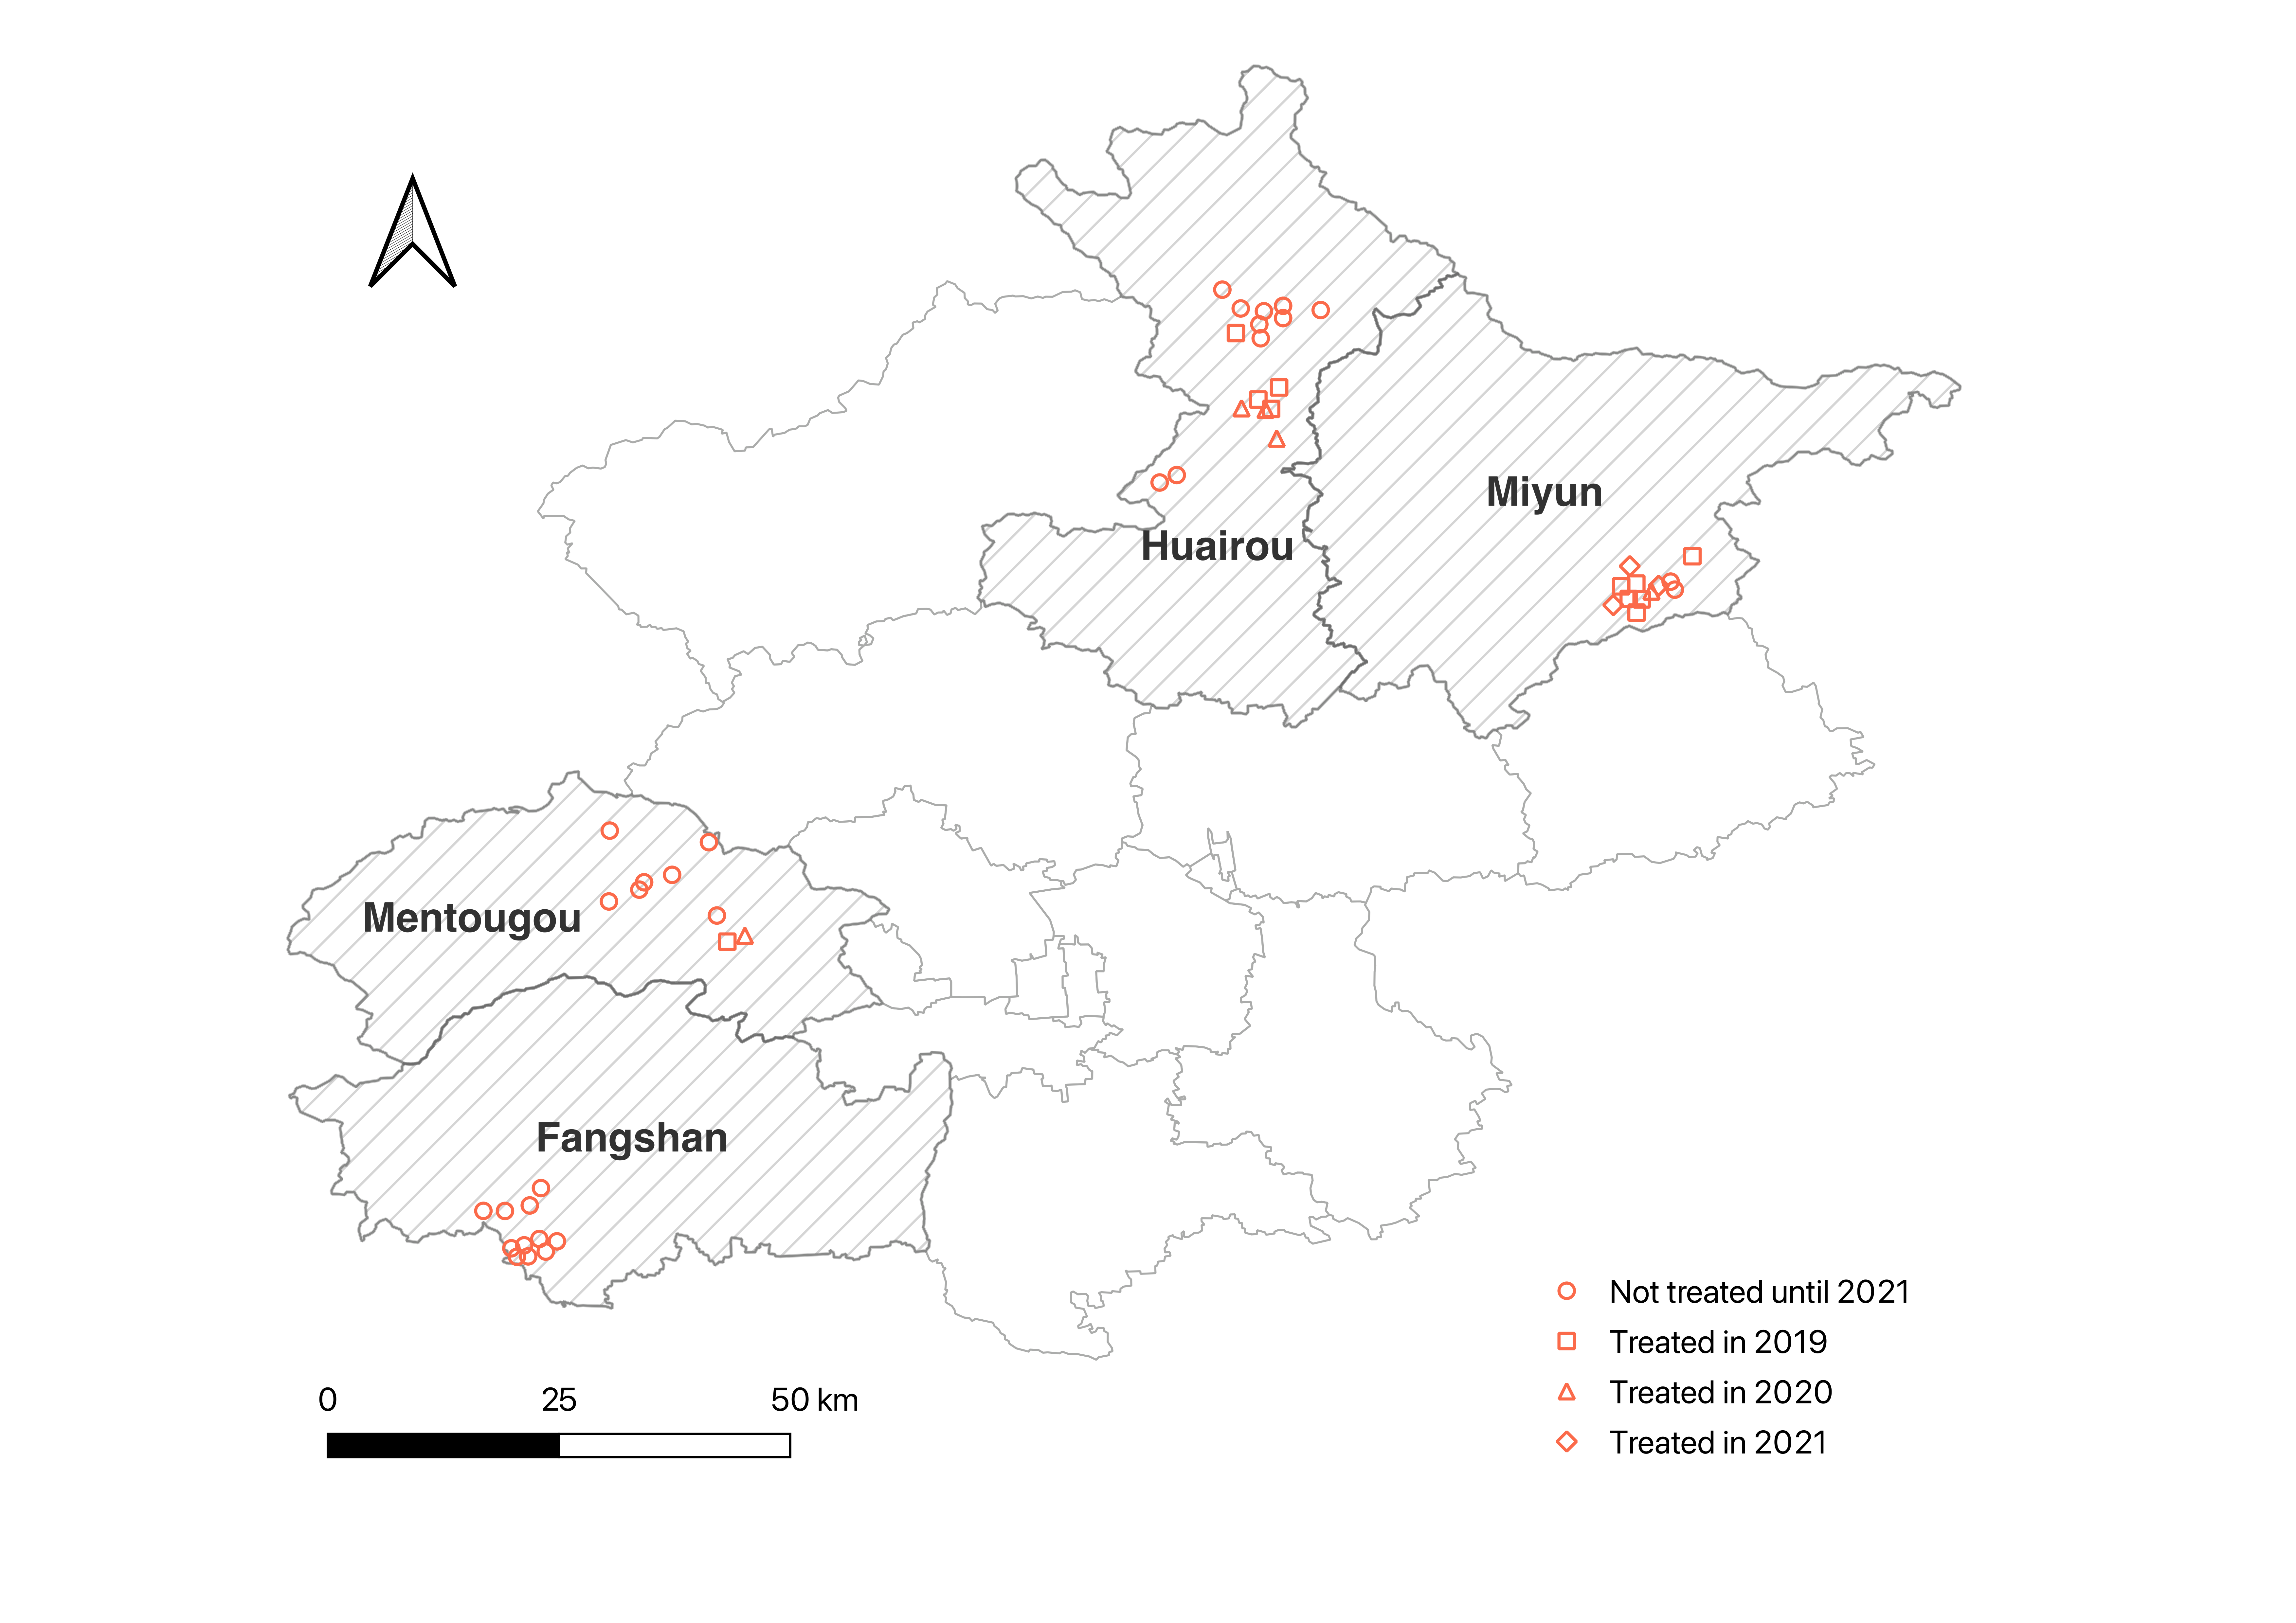
\includegraphics[width=0.7\textwidth,height=\textheight]{images/policy-implementation-map.png}

}

\caption{\label{fig-cbhp-map}Map of village implementation of CBHP
policy}

\end{figure}

We recruited approximately 20 households in each village and randomly
selected one eligible person from each household to participate.
Household members were eligible to participate if they were over 40
years old, lived in the study villages, were not planning to move out of
the village in the next year, and were not on current immunotherapy or
treatment with corticosteroids. Research staff introduced the study and
its measurements to an eligible adult in each household and answered any
questions related to the study. In follow-up visits to the study
villages, staff first approached households with participants from an
earlier campaign. If previous participants were not at home or refused
to participate, staff first tried to randomly recruit an eligible
participant from the same household. If there was not another eligible
or willing participant in the household, we randomly selected and
recruited a participant from a new household using the village roster.
All participants provided written informed consent prior to joining the
study. The study protocols were approved by research ethics boards at
Peking University (IRB00001052-18090) and McGill University
(A08-E53-18B).

\hypertarget{data-collection-overview}{%
\subsection{Data Collection Overview}\label{data-collection-overview}}

We conducted study measurements over four consecutive winter seasons in
2018-19, 2019-20, 2020-21, and 2021-22 (referred to in this Report as
S1, S2, S3 and S4, respectively). Field data collection was conducted by
\textasciitilde20 trained staff members who traveled to participants'
homes to conduct tablet-based household and individual questionnaires,
measure participant blood pressure, and distribute temperature sensors
(for measurement of indoor temperature and stove use) and air pollution
monitors in all 50 study villages in S1, S2, and S4. Anthropometrics
(height, weight, and waist circumference), measurement of airway
inflammation, and whole blood samples were obtained no more than a month
later at a village clinic in S1 and S2. In S3, which was during the
height of the pandemic, we limited household measurements to indoor air
quality and sensor-based measurement of indoor temperature and stove use
in 41 villages, including all 17 treated villages and 24 untreated
(control) villages, prior to COVID-related travel restrictions that
halted field data collection. In S4, which also occurred during the
COVID-19 pandemic, we returned to conducting individual-level
assessments. However, unlike in S1 and S2, anthropometric measurements
and airway inflammation were assessed in participant homes rather than
clinics to avoid group contact and blood samples were not collected.
Outdoor (community) air pollution was measured throughout the study
period.

\hypertarget{air-pollution}{%
\subsubsection{Air Pollution}\label{air-pollution}}

\hypertarget{outdoor-air-pollution}{%
\paragraph{Outdoor air pollution}\label{outdoor-air-pollution}}

In each village, two sensors for particulate matter air pollution were
set up to measure outdoor (community) PM\textsubscript{2.5} at different
locations in each village. One sensor was placed near the center of the
village, and the other was placed no less than 500m away from the
centrally-located sensor. Sensors were placed at least 1.5m above the
ground and not in a location within sight of a visible point source of
PM\textsubscript{2.5}.

We collected filter-based community PM\textsubscript{2.5} samples to
calibrate the sensor-based PM\textsubscript{2.5} measurements as well as
to conduct analysis of chemical composition for source apportionment.
Ultrasonic Personal Aerosol Samplers (UPAS, Access Sensor Technologies,
Fort Collins, CO, USA) were used to collect filter-based
PM\textsubscript{2.5} samples with a flow rate of 1.0 L/min (Volckens et
al. 2017). Samplers housed 37mm PTFE filters (VWR, 2.0-μm pore size) and
were equipped with a cyclone inlet with a 2.5μm cut point designed to
perform under the sampling flow rate. For community measurements, a UPAS
was co-located with each PM\textsubscript{2.5} sensor in each village in
rotation. Every week, the used filters were removed and replaced with a
new filter. In total, we successfully collected 126, 371, and 289
filter-based, community outdoor PM\textsubscript{2.5} samples in Seasons
1, 2, and 4, respectively. Field blank filters were collected at a rate
of \textasciitilde10\%, subject to the same field conditions as samples.
To support post-sampling determination of organic carbon (OC) and
elemental carbon (EC) fractions of PM\textsubscript{2.5} mass, quartz
filters were co-located with a subset of Teflon filter samples collected
outdoors. Filter-based PM\textsubscript{2.5} samples were collected
using Personal Exposure Monitors (PEMs, Apex Pro) operating with flow
rates of 1.8 L/min. PEMs housed 37 mm quartz filters (VWR, 2.0-μm pore
size) and were equipped with a cyclone inlet with a 2.5 μm cut point
designed to perform under the corresponding sampling flow rate. All
quartz fiber filters were baked at 550 C for a minimum of 8 h to remove
organic impurities prior to sample collection. PM\textsubscript{2.5}
samples collected on quartz filters were analyzed using established
thermo-optical methods for quantifying elemental carbon (EC) and organic
carbon (OC) to, then, calibrate the colorimetric analysis of EC and OC
on Teflon filters. In Season 2, 23 quartz-based outdoor
PM\textsubscript{2.5} samples and 3 field blanks were collected. In
Season 4, 11 quartz-based outdoor PM\textsubscript{2.5} samples and 3
field blanks were collected.

For PM\textsubscript{2.5} sensor calibration and quality control, all PM
sensors were co-located with a reference-grade PM\textsubscript{2.5}
instrument (Model 5030 Synchronized Hybrid Ambient Realtime Particulate
(SHARP) Monitor, Thermo Fisher Scientific, United States) on the rooftop
of a building at Peking University campus for 7 to 10 days before and
after each field campaign (Figure~\ref{fig-calibration}).
Sensor-measured PM\textsubscript{2.5} concentrations were highly
correlated with those measured by the SHARP (Spearman correlation
coefficients (rho) of 0.95 and 0.82 in pre- and post-calibration,
respectively).

\begin{figure}[H]

{\centering 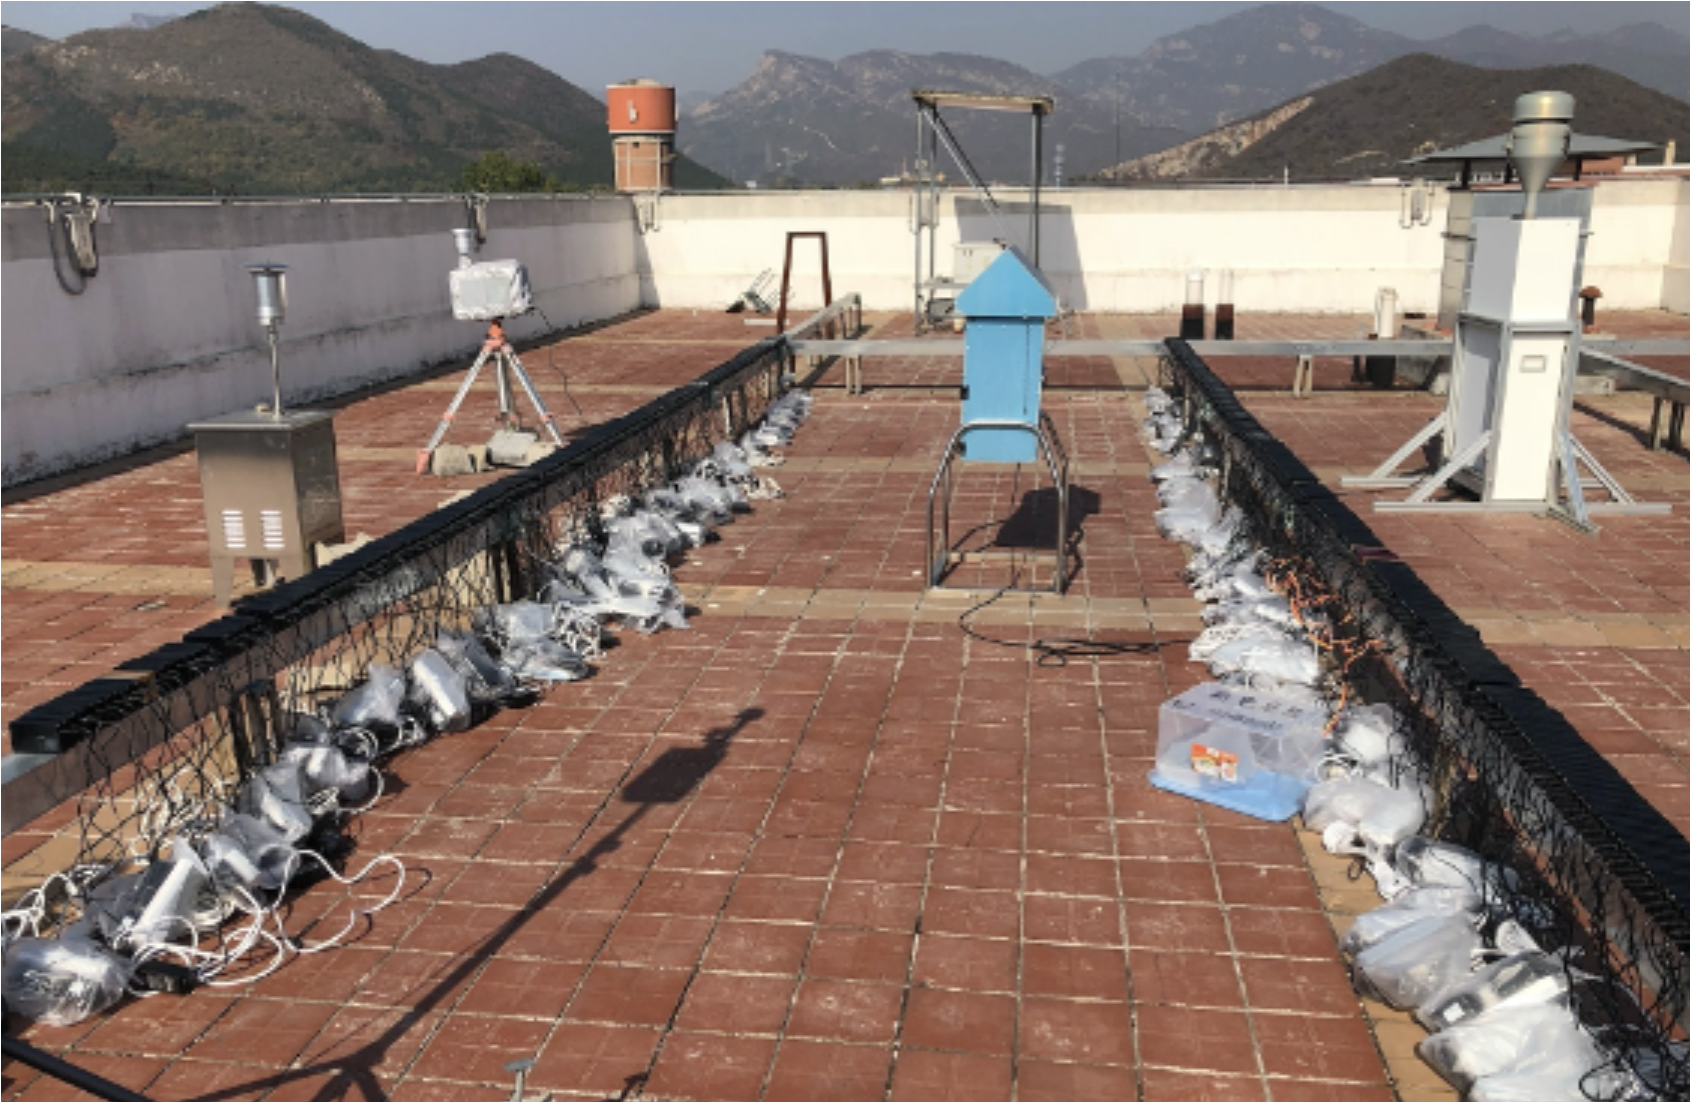
\includegraphics[width=0.8\textwidth,height=\textheight]{images/sensor-calibration.png}

}

\caption{\label{fig-calibration}Calibration of real-time sensors against
a reference monitor at University of the Chinese Academy of Sciences.}

\end{figure}

\hypertarget{indoor-pm2.5}{%
\paragraph{\texorpdfstring{Indoor
PM\textsubscript{2.5}}{Indoor PM2.5}}\label{indoor-pm2.5}}

In the second and fourth field seasons (i.e., S2 and S4), we randomly
selected six households from the 20 recruited in each village to measure
indoor concentrations of PM\textsubscript{2.5}. In Season 4, we aimed to
monitor indoor PM\textsubscript{2.5} in the same households where we
measured indoor PM\textsubscript{2.5} in Season 2. If a household
dropped out of the project or declined indoor PM\textsubscript{2.5}
monitoring, we then recruited another household already enrolled in this
study to measure indoor PM\textsubscript{2.5}. In total, indoor
measurements were conducted in 300 households in both Season 2 and
Season 4 (Table~\ref{tbl-pm-sample}).

\hypertarget{tbl-pm-sample}{}
\begin{table}
\caption{\label{tbl-pm-sample}Household recruitment for overall and indoor air quality measurements. }\tabularnewline

\centering
\begin{tabular}{lrrrrrr}
\toprule
\multicolumn{1}{c}{ } & \multicolumn{3}{c}{Overall} & \multicolumn{3}{c}{Indoor} \\
\cmidrule(l{3pt}r{3pt}){2-4} \cmidrule(l{3pt}r{3pt}){5-7}
Sample & Season 1 & Season 2 & Season 4 & Season 1 & Season 2 & Season 4\\
\midrule
New recruitment & 977 & 0 & 196 & 300 & 68 & 52\\
Households from Season 1 & \textbackslash{} & \textbackslash{} & 866 & 0 & 780 & 0\\
Households from Season 2 & \textbackslash{} & \textbackslash{} & \textbackslash{} & \textbackslash{} & 162 & 248\\
Total recruitment & 977 & 0 & 1062 & 300 & 1010 & 300\\
\bottomrule
\end{tabular}
\end{table}

Time-resolved indoor PM\textsubscript{2.5} concentrations were measured
using the same commercially available sensor (PMS7003 Plantower, Zefan,
Inc.) as was used for outdoor sensor-based PM\textsubscript{2.5}
measurements and recorded PM\textsubscript{2.5} concentrations every 1
min. The sensor was placed on a table in a room where participants
reported spending most of their time when awake, e.g., a living room or
bedroom. Indoor PM\textsubscript{2.5} sensors were deployed between late
November and mid January within field seasons (i.e., S2 and S4),
depending on the village and household visit schedule. The measurement
continued from the time of deployment until sensors were recollected
from homes in late April to capture the full heating season.

We randomly selected three households from the six households in which
we deployed PM\textsubscript{2.5} sensors to co-locate a filter-based
PM\textsubscript{2.5} sampler with the PM\textsubscript{2.5} sensor. We
collected a 24-h PM\textsubscript{2.5} filter sample at the first 24-h
of indoor PM\textsubscript{2.5} sensor measurements. Filter-based
PM\textsubscript{2.5} samples were collected using Ultrasonic Personal
Aerosol Samplers (UPAS, Access Sensor Technologies) or Personal Exposure
Monitors (PEMs, Apex Pro) operating with flow rates of 1.0 and 1.8
L/min, respectively. Both samplers housed 37 mm PTFE filters (VWR,
2.0-μm pore size) and were equipped with a cyclone inlet with a 2.5 μm
cut point designed to perform under the corresponding sampling flow
rate. After 24-h, the samplers were retrieved and loaded with new
filters for measurements in other villages, once the previous sample
filters were removed and stored for later analysis. In total, we
successfully collected 149 and 148 indoor PM\textsubscript{2.5} filter
samples in S2 and S4, respectively.

As with the community outdoor air sampling, to support post-sampling
determination of organic carbon (OC) and elemental carbon (EC) fractions
of PM\textsubscript{2.5} mass, quartz filters were co-located with a
subset of Teflon filter samples collected in homes. Filter-based
PM\textsubscript{2.5} samples were collected using Personal Exposure
Monitors (PEMs, Apex Pro) operating with flow rates of 1.8 L/min. PEMs
housed 37 mm quartz filters (VWR, 2.0-μm pore size) and were equipped
with a cyclone inlet with a 2.5 μm cut point designed to perform under
the corresponding sampling flow rate. All quartz fiber filters were
baked at 550 C for a minimum of 8 h to remove organic impurities prior
to sample collection. PM\textsubscript{2.5} samples collected on quartz
filters were analyzed using established thermo-optical methods for
quantifying elemental carbon (EC) and organic carbon (OC) to, then,
calibrate the colorimetric analysis of EC and OC on Teflon filters. In
Season 2, 71 quartz-based indoor PM\textsubscript{2.5} samples and 14
field blanks were successfully collected. In Season 4, indoor
PM\textsubscript{2.5} samples for gravimetric analysis had to be
collected on two types of PTFE sample media (Zefluor and Teflo filters),
due to discontinuation of manufacturing of the Zefluor filter media. To
ensure that quartz filters were deployed with both types of Teflon-based
filter media, 73 quartz-based indoor PM\textsubscript{2.5} samples were
collected concurrently with Zefluor samples, and 47 quartz indoor
PM\textsubscript{2.5} samples were collected alongside Teflo samples.
For indoor quartz PM\textsubscript{2.5} mass sampling in S4, 18 field
blanks were collected.

\hypertarget{personal-exposure-to-pm2.5-and-black-carbon}{%
\paragraph{\texorpdfstring{Personal exposure to PM\textsubscript{2.5}
and black
carbon}{Personal exposure to PM2.5 and black carbon}}\label{personal-exposure-to-pm2.5-and-black-carbon}}

To measure personal exposure we used two types of samplers: Personal
Exposure Monitors (PEMs, Apex Pro; Casella, UK) and Ultrasonic Personal
Aerosol Samplers (UPAS, Access Sensor Technologies, Fort Collins, CO,
USA). PEMs actively sampled air at a flow rate of 1.8 L/min, and UPAS
sampled air at 1.0 L/min (Volckens et al. 2017). Both samplers housed 37
mm PTFE filters (VWR, 2.0-μm pore size) and were equipped with a cyclone
inlet with a 2.5 μm cutpoint. Sampler flow rates were calibrated the
night before deployment and measured immediately after the sampling
period. Only 2\% of the post-sampling measurements deviated from the
target flow rate by greater than +/-10\%. Participants were instructed
to wear a small waistpack (for the PEM and sampling pump) or an arm band
or cross-body sling (for the UPAS) for 24 hours, which they could remove
from their body and place within 2 meters while sleeping, sitting, or
bathing. Field blanks for personal air pollution exposure measurements
were collected at a rate of \textasciitilde10\% in each village.

\hypertarget{gravimetric-analyses-of-ptfe-filter-based-pm2.5-samples}{%
\subsubsection{\texorpdfstring{Gravimetric analyses of PTFE filter-based
\textsubscript{PM2.5}
samples}{Gravimetric analyses of PTFE filter-based PM2.5 samples}}\label{gravimetric-analyses-of-ptfe-filter-based-pm2.5-samples}}

All filters were placed in individually labeled cases, sealed in plastic
bags, and then transported to a field laboratory and immediately stored
in a -20°C freezer. Following completion of the field sampling campaign,
the samples and blanks were transported to Colorado State University,
where they were stored in a -20°C freezer prior to PM\textsubscript{2.5}
mass measurement and chemical analysis of PM.

All filters were placed in an environmentally-controlled equilibration
chamber (21-22 °C, 30-34\% relative humidity) for at least 24 hours
before tare and gross weighing. Before each weight was taken, filters
were discharged by a polonium-210 strip. Filters were weighed on a
microbalance (Mettler Toledo Inc., XS3DU, USA) with 1-μg resolution in
triplicate or more, until the differences among three weights were less
than 3 μg. The average of three readings was used to determine filter
mass, which was then blank-corrected using the median value of blank
filters {[}3 μg for UPAS-collected filters (53\% of samples); 33 μg for
PEM-collected filters (47\% of filter samples){]}, and PM2.5
concentrations were calculated by dividing the mass by the sampled air
volume.

\hypertarget{adjusting-sensor-based-pm2.5-using-filter-based-gravimetric-measurements}{%
\paragraph{\texorpdfstring{Adjusting sensor-based PM\textsubscript{2.5}
using filter-based gravimetric
measurements}{Adjusting sensor-based PM2.5 using filter-based gravimetric measurements}}\label{adjusting-sensor-based-pm2.5-using-filter-based-gravimetric-measurements}}

We established linear regression models between the filter-based
PM\textsubscript{2.5} mass concentrations (i.e., the `gold standard'
reference concentrations) and the sensor-based PM\textsubscript{2.5}
concentrations averaged over the same sampling period as the
filter-based samples. The slopes of the models were used as the
adjustment factors for the sensor-based PM\textsubscript{2.5}
concentrations. Separate regression models were conducted for indoor and
outdoor sensors and for each season given the sensitivity of the sensors
to relative humidity, temperature, and particle sources, which may
differ for indoor versus outdoor conditions and across seasons. In
Season 3, where only sensor-based measurements were conducted for indoor
PM\textsubscript{2.5} to avoid direct contact with household members
during the pandemic, we applied an adjustment factor developed from a
linear regression model that incorporated data from both Season 2 and
Season 4.

The PM sensors were also evaluated before and after each season to
identify any sensors that needed further repair or replacement. The
PM\textsubscript{2.5} sensors underwent a calibration process that began
with synchronization to real-time PM2.5 monitors at Peking University
(PKU) campus. This pre- and post-season calibration included a week-long
session using the Beta Attenuation Monitor (BAM) alongside daily 24-hour
filter samples. During this time, approximately 240 sensors were placed
on the rooftop of the College of Urban and Environmental Sciences
building, each recording data every minute. A similar approach was taken
at the University of Chinese Academy of Sciences (UCAS) campus, where
around 400 PM sensors were installed on the rooftop of the Environmental
Monitoring Site of the College of Resources and Environment, with data
logging at one-minute intervals. Daily collections of 24-hour Zeflour
(Teflon) and quartz filter samples accompanied the sensors' measurements
to ensure accuracy. The calibration process was repeated post-fieldwork
to account for any potential shifts or discrepancies in sensor
performance. This approach aimed to maintain consistent and accurate
measurements from the PM sensors throughout the study.

\hypertarget{chemical-analysis-of-pm-mass}{%
\subsubsection{Chemical analysis of PM
mass}\label{chemical-analysis-of-pm-mass}}

We analyzed the chemical composition of community outdoor and personal
exposure PM\textsubscript{2.5} samples from each season to quantify the
individual components and species. PM\textsubscript{2.5} component
concentrations were determined within each community by dividing the
quantified component mass by the sampled air volume, after correcting
for field blanks collected in the corresponding season.

Elemental analysis of PM\textsubscript{2.5} mass was performed using a
Thermo Scientific Quant'X Evo energy-dispersive X-ray fluorescence
(EDXRF) spectrometer with Wintrace software version 10.3 using standard
methods (International 2009). Quantitative mass concentrations of 22
individual elements (Mg, Al, Si, S, K, Ca, Ti, Cr, Mn, Fe, Ni, Cu, Zn,
Ga, As, Se, Cd, In, Sn, Sb, Te, I) were determined empirically using
linear standard curves. Standard curves were generated from commercial,
single and dual element, thin film standards from MicroMatter
Technologies Inc.~(Montreal, Canada) in addition to blank films. The
quality of the analysis method was evaluated by analyzing a National
Institute of Standards and Technology (NIST) standard reference material
(SRM) 2783 Air particulate on filter media (Gaithersburg, MD, USA).
Elements for which at least 80\% of PM\textsubscript{2.5} mass samples
yielded quantifiable element mass were included for positive matrix
factorization and source analysis and apportionment. Those elements
were: Si, Mg, Fe, S, Ca, Al, K, Pb.

For analysis of water-soluble ions, a portion of each PTFE filter was
extracted in 15 mL deionized water (DI Water) in a Nalgene Amber HDPE
bottle using sonication without heat for 40 min. The extracts were
filtered to ensure that insoluble particles were removed using a 0.2 μm
PTFE syringe filter. Water-soluble ions were measured using a dual
channel Dionex ICS-3000 ion chromatography system. Specifically, a
Dionex IonPac CS12A analytical (3 × 150 mm) column with eluent of 20 mM
methanesulfonic acid at a flow rate of 0.5 mL/min was used to measure
cations (Ca2+, Mg2+, Na+, NH4+, K+), while a Dionex IonPac AS14A
analytical (4 × 250 mm) column with an eluent of 1 mM sodium
bicarbonate/8 mM sodium carbonate at a flow rate of 1 mL/min was used to
measure anions (SO42−, NO3−, Cl−) (Sullivan et al., 2008).

Organic (OC) and elemental carbon (EC) on PTFE filters were measured
using an optical color space sensing system. The CIE-Lab color space
optical sensing system measures the optical properties of the
PM\textsubscript{2.5} samples, and these properties are used to develop
the EC and OC predictive models. The CIE-Lab color system is a
color-opponent space that includes all of the color models, with
dimension L* for lightness and a* and b* for the color-opponent
dimensions. More information about the CIE Lab color space system, its
formulation, and its specific application to the analysis of OC and EC
fractions of fine particulate matter pollution is provided in Khuzestani
et al. (Khuzestani et al. 2017). Briefly, all the Teflon (PTFE) and
quartz filters collected were analyzed using the i1Pro Colorimeter
(X-Rite, INC. Grand Rapids, MI). The colorimeter sensor was placed
directly over the quartz and Teflon filters, and the color components
were measured under the D65 instrument internal illumination light
source. Each filter sample was analyzed in triplicate, and the average
value of each color coordinate was applied as the optical property of
the sample (Olson et al. 2016). CIE Standard Illuminant D65 simulates
average midday light and is a commonly used standard illuminant, as
defined by the International Commission on Illumination (CIE). The
CIE-Lab color space response variables were used in separate random
forest models for EC and OC.

The reference measurements for the random forest model development were
EC and OC determined from quartz filters collected indoors and outdoors
(as described above). PM\textsubscript{2.5} samples collected on quartz
filters were analyzed for OC and EC using a Sunset Laboratory OC/EC Lab
instrument (Sunset Laboratories, Inc., MODEL, USA) according to the
default Sunset Analyzer protocol. A section of each quartz filter
underwent a combined thermal desorption-optical transmittance
measurement based on NIOSH methods 5040 to differentiate and quantify
the EC and OC components in mass. For the thermal desorption component,
the sample is oxidized twice, according to a strict temperature regime.
The first oxidation stage thermally removes OC in a mobile phase of pure
helium gas to be converted from carbon dioxide (CO2) to methane (CH4)
gas and measured by a flame ionization detector (FID). The second
oxidation stage proceeds in a mixture of helium and oxygen to oxidize
EC, which is also quantified by the FID. The FID is internally
calibrated with methane, and external quality control checks are made
with sucrose standards. To correct for the potential production of EC by
OC pyrolysis during the first heating stage, light transmission from a
laser through the filter section was monitored throughout analysis.
Reduced light transmittance corresponds to EC generated by the
laboratory analysis.

Following gravimetric analysis, all PTFE filters were also analyzed for
black carbon (BC) using an optical transmissometer data acquisition
system (SootScan\^{}TM OT21 Optical Transmissometer; Magee Scientific,
Berkeley, CA, USA). Light attenuation through each filter was measured
before and after sampling in the field. To calculate BC mass, the
difference between the pre- and post- light attenuation was converted to
a mass surface loading using the classical Magee mass absorption
cross-sections of 16.6 m2/g for the 880 nm channel optical BC (Ahmed et
al. 2009). BC concentrations were calculated by multiplying surface
loadings by the sampled surface area of the filters (8.6 cm2 for
UPAS-collected filters; 7.1 cm2 for PEM-collected filters), correcting
for the field blank mass using the median value of blanks (0.31 μg for
UPAS-collected filters; 0.01 μg for PEM-collected filters), and finally
dividing by the sampled air volume.

\hypertarget{outdoor-and-indoor-household-air-temperature}{%
\subsubsection{Outdoor and indoor (household) air
temperature}\label{outdoor-and-indoor-household-air-temperature}}

Hourly outdoor temperature and relative humidity data were obtained from
the extensive network of meteorological
\href{http://beijingair.sinaapp.com}{stations} in Beijing. We measured
indoor temperature in all participant homes prior to blood pressure
measurement. In a random 75\% subsample of households in each campaign,
we also placed a real-time temperature sensor (iButton DS1921G-F5;
Thermochron, Maxim Inc., USA) in the room where participants reported
spending most of their daytime hours when indoors. Sensors were
wall-mounted at a standardized height (\textasciitilde1.5 to 2 meters),
away from major heating sources, windows, and doors, and were programmed
to log a temperature reading every 125 minutes for up to 4 months to
capture the full winter period and early spring weeks when heating may
still intermittently occur. Prior to the start of each campaign, we
co-located all of the sensors and measured temperature over two days and
compared the readings. Sensors recording values \textgreater1C from the
group median value were excluded from data collection.

\hypertarget{objective-measurement-of-household-stove-use-using-sensors}{%
\subsubsection{Objective measurement of household stove use using
sensors}\label{objective-measurement-of-household-stove-use-using-sensors}}

Following methods used in a previous intervention evaluation study in
rural China (Clark et al. 2017), we objectively measured household
heating stove use in a random sample of households selected, also at
random, for either short- or long-term measurement. We measured
short-term (24 h) stove use for all household heating stoves in 315 and
227 households in seasons 2 and 3, respectively. Long-term stove use was
assessed in 324, 273, and 585 homes in S2, S3, and S4, respectively, for
a period of approximately 6 months. We measured stove use using the same
real-time temperature data loggers used for indoor temperature (iButton
DS1921G-F5; Thermochron, Maxim Inc., USA). Field staff placed the
sensors on stoves and programmed them to record surface temperature
every 125 minutes, a timing decision based on pilot assessments showing
that shorter time intervals did not change the number of heating events
detected. Sensors were on the surfaces of biomass and coal-fuelled
stoves and radiators. For heat pumps, sensors were placed on the heat
exchanger coil on air-to-air units and on the radiator of air-to-water
units.

The number and duration of stove combustion events were identified from
the temperature data using criteria defined based on the observed
changes in the peak shape of the time series temperature curves (i.e.,
changes in the slope or in absolute temperature compared with the indoor
ambient temperature). This approach was specific to heating stoves but
developed based on stove use identification for cookstoves in previous
studies by us and others (Clark et al. 2017; Ruiz-Mercado et al. 2013;
Snider et al. 2018). We developed separate criteria for each stove since
heating patterns varied by stove. These criteria were coded into
stove-specific algorithms (using R Studio) to systematically identify
the number and duration of heating events across households. A random
15\% of stove use temperature files were sampled with respect to the
stove type and measurement duration (short-term/24 h or
long-term/\textasciitilde6 mo), and manually coded to develop the
criteria. The number and duration of heating events were identified by
the algorithms in the remaining 85\% of files. We compared heating
periods identified manually with those identified by the algorithm to
check for systematic differences and possible overfitting.

\hypertarget{questionnaires}{%
\subsubsection{Questionnaires}\label{questionnaires}}

Field staff administered household and individual-level questionnaires
to assess household demographic information and educational attainment,
household assets, house structure, stove and fuel use patterns
(including a complete roster of heating methods and their contributions
in each room), and individual health behaviors including exercise
frequency, smoking, alcohol consumption, medication use, and
clinician-diagnosed health conditions. We used Surveybe
computer-assisted personal interview (CAPI) software to collect survey
data via handheld electronic tablets. Questions were read to
participants in Mandarin-Chinese, and their responses were recorded into
tablets.

Prior to the start of data collection, all questions were translated
from English into Chinese and then back-translated to English for
quality assurance. Many questions were adapted from previous field
studies of household energy and blood pressure conducted in rural
Beijing or other rural sites in China (Baumgartner et al. 2018; Yan et
al. 2020), and all questions were iteratively tested with staff and
adapted prior to implementation. Prior to each campaign in this study,
the questionnaire and other study measurements were tested in 12
households located in a Beijing village that was eligible for our study
but was instead selected for testing. We used the test village to assess
whether the questions were understandable and interpreted as intended
and to identify any problems with the study measurements or their
implementation. Study protocols were subsequently adapted prior to the
start of data collection.

In addition to household and individual participant questionnaires, we
also conducted village surveys with one representative from each village
committee to inquire about any other policies or programs being
implemented in the village (e.g., biomass burning bans) and to
understand how the policy was implemented in that village. Committee
members answered questions about assignment versus application to the
policy, any renovations required by the upper-level government, level of
subsidies provided for heating stoves and electricity, and technical and
logistic guidance to villagers.

\hypertarget{blood-pressure}{%
\subsubsection{Blood pressure}\label{blood-pressure}}

Following 5 min of quiet rest, at least three brachial and central
systolic (bSBP/cSBP) and diastolic (bDBP/cDBP) blood pressures (BPs)
were taken by trained staff at 1 min apart on the participant's
supported right arm. We used an automated oscillometric device (BP+;
Uscom Ltd, New Zealand) that estimates central pressures from the
brachial cuff pressure fluctuations. Central pressures were previously
validated against invasive cBP measurements in previous studies
(Costello et al. 2015; Lowe et al. 2009). The BP devices were factory
calibrated by the manufacturer prior to the start of the first and
fourth campaigns. Up to five measurements were taken if the difference
between the last two was \textgreater5 mmHg or staff were unable to
obtain a reading. The BP measurements were conducted in the
participant's home and staff were trained to follow strict quality
control procedures, including use of an appropriately sized cuff,
correct positioning of the arm, both feet on the ground, and ensuring 5
min of quiet rest before measurement. Details are described in the
standard operating procedures (SOP): https://osf.io/gmka5. The average
of the final two measurements was used for statistical analysis unless
only one BP measurement was obtained (n = 13 observations), in which
case, a single measurement was used. The time of day, day of the week,
and indoor temperature prior to BP measurement were also recorded.

\hypertarget{multiple-imputation-for-covariates-in-analyses-with-bp-outcomes}{%
\paragraph{Multiple imputation for covariates in analyses with BP
outcomes}\label{multiple-imputation-for-covariates-in-analyses-with-bp-outcomes}}

Blood pressure was measured at household visits but several key
covariates like waist circumference, height, and weight were measured at
the clinic visits in S1 and S2. Thus, we were missing covariate
information for individuals who were unable to attend the clinic visits
(\textasciitilde15-20\% of participants in each campaign). Multiple
imputation with chained equations (MICE) was conducted to impute missing
covariate data for individuals who participated in the household visit
but not the clinic visit in analyses with BP outcomes in order to retain
observations with BP measurements that would have otherwise been dropped
in adjusted models using complete-case analysis. Imputation was
performed with the `MICE' package (van Buuren and Groothuis-Oudshoorn
2011) in R (m = 30 imputation datasets, with 30 iterations each), and
the DiD analysis was conducted for each of the 30 datasets. We then used
Rubin's Rules to combine point estimates and standard errors while
accounting for both within- and between-dataset variances (Rubin 1987).

\hypertarget{self-reported-respiratory-symptoms-and-airway-inflammation}{%
\subsubsection{Self-reported respiratory symptoms and airway
inflammation}\label{self-reported-respiratory-symptoms-and-airway-inflammation}}

During questionnaire assessment, participants were asked about chronic
airway symptoms including cough, phlegm, wheeze, and tightness in the
chest using questions validated for use in Mandarin-Chinese and
developed from the standard questionnaires on COPD (Medical Research
Council/International Union Against Tuberculosis and Lung Disease) and
asthma (International Study of Asthma and Allergies in Childhood). The
Mandarin-Chinese questions were extensively piloted with rural and
peri-urban Beijing residents to ensure that the health terminology and
symptom time patterns were adequate and understandable to the local
population.

In a \textasciitilde25\% random subsample of participants, we also
measured fractional exhaled nitric oxide (FeNO), a non-invasive and
established marker of airway inflammation, using a portable handheld
device (Aerocrine, Solna, Sweden) fit with a NIOX VERO® sensor,
following ATS recommendations and guidelines (ATS/ERS 2005). Briefly,
FeNO measurement was performed with participants in a standing position.
They inhaled NO-free air through a mouthpiece with an NO-scrubber
attached, followed by controlled expiration for 10 s through the
mouthpiece at 50±5 mL/s. A nose clip was used to avoid nasal inhalation,
and accurate flow rate was achieved using visual and auditory cues
generated by the device. Detailed methods are provided in our previous
study of air pollution and FeNO in Beijing adults (Shang et al. 2020).
At least two measurements were obtained for each participant.

\hypertarget{blood-inflammatory-and-oxidative-stress-markers}{%
\subsubsection{Blood inflammatory and oxidative stress
markers}\label{blood-inflammatory-and-oxidative-stress-markers}}

Trained nurses collected 4 ml of whole blood in a labeled vacutainer via
venipuncture using standard techniques (Tuck 2009). Details are
descriptive in the SOP: https://osf.io/zwpfg. Briefly, fasting blood
samples were collected by experienced phlebotomists (nurses) in the
morning and stored at 4-10°C prior to centrifugation. Two serum aliquots
from each participant were then placed in a -30°C freezer for temporary
storage. Collection-to-storage time was \textless4 hrs for all samples
in both campaigns where blood samples were collected. Within 3-5 days of
collection, the samples were transported in styrofoam containers with
dry ice to a -80°C freezer with a backup generator and alarm system at
Peking University.

The first aliquot was analyzed for glucose and a complete lipid profile
within two months of collection, and results were communicated to
participants. The second aliquot was stored in the -80°C freezer for
analysis of biomarkers of systemic inflammation {[}C-reactive protein
(CRP), interleukin-6 (IL-6), tumour necrosis factor alpha (TNF-ɑ{]} and
oxidative stress {[}8-hydroxy-2'-deoxyguanosine (8-OHdG) and
malondialdehyde (MDA){]} at the University of the Chinese Academy of
Sciences between July and September of 2023. These biomarkers were
selected because they are associated with the development of
cardiovascular disease and events (e.g., Danesh 2008; Pearson 2003;
Ridker 2000; 2001; ERF 2012), and both acute and longer-term exposures
to air pollution have been associated with changes in inflammatory and
oxidative stress markers (e.g., Pope 2004; Rückerl 2007; Rich 2012;
Kipen 2010; Huang 2012).

We followed standard methods for analysis (FDA Guidance, 2018). For
inflammatory markers (IL-6, TNF-α, CRP), the optic densities (OD) of all
samples were measured using an automated ELISA reader. Every plate had 8
standard samples used to generate a standard curve that related OD and
standard inflammatory marker concentration. A standard curve for each
microplate was generated by a computer software program based on a
4-parameter method. Each plate included at least 3 control samples to
ensure the stability of standard curves. All samples, standards, and
controls were measured in duplicate, and the average was used for
statistical analysis. For oxidative stress biomarkers (MDA and 8-OHdG),
the chromatographic peak areas of all samples were measured using HPLC
with UV detector and HPLC-MS/MS. Every plate had 7 standard samples used
to generate a standard curve that related peak area and concentration of
each standard oxidative stress marker. A standard curve for each plate
was generated using a computer software program based on a linear
method. Each plate included at least 3 control samples to ensure the
stability of standard curves. Standards and controls were measured in
duplicate and samples were measured once due to high precision in a
pilot study (Food and Drug Administration 2018).

\hypertarget{anthropometric-measurements.}{%
\subsubsection{Anthropometric
measurements.}\label{anthropometric-measurements.}}

Body weight, height, and waist circumference were measured at the clinic
visit in the first two campaigns and in participant homes in the last
campaign. Weight was measured in light indoor clothing without shoes in
kilograms to one decimal place, using standing scales supported on a
steady surface. The scales were calibrated prior to the start of each
campaign, and the same staff member stepped on the scale each morning to
ensure that it was functioning properly. Height was measured without
shoes in centimeters to one decimal place with a stadiometer. Waist
circumference was measured without clothing obstruction at 1 cm above
the participant's navel at minimal respiration in centimeters to one
decimal place. The measuring tape was replaced at the start of each
campaign to avoid stretching.

\hypertarget{measuring-policy-impacts}{%
\subsection{Measuring policy impacts}\label{measuring-policy-impacts}}

To understand how Beijing's policy works we used a
difference-in-differences (DiD) design (Callaway 2020), leveraging the
staggered rollout of the policy across multiple villages to estimate its
impact on health outcomes and understand the mechanisms through which it
works. Simple comparisons of treated and untreated (i.e., control)
villages after the CBHP policy has been implemented are likely to be
biased by unmeasured village-level characteristics (e.g., migration,
average winter temperature) that are associated with health outcomes.
Similarly, comparisons of only treated villages before and after
exposure to the program are susceptible to bias by other factors
associated with changes in outcomes over time (i.e., secular trends,
impacts of the COVID-19 pandemic). By comparing \emph{changes} in
outcomes among treated villages to \emph{changes} in outcomes among
untreated villages, we can control for any unmeasured time-invariant
characteristics of villages as well as any general secular trends
affecting all villages that are unrelated to the policy.

\begin{figure}[H]

{\centering 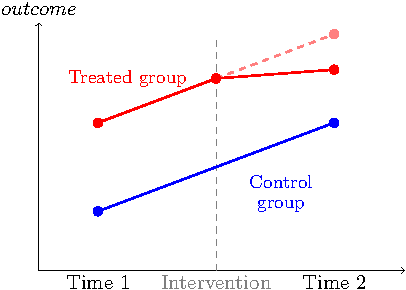
\includegraphics[width=0.5\textwidth,height=\textheight]{hei-report_files/figure-pdf/fig-didfig-1.pdf}

}

\caption{\label{fig-didfig}Stylized example of
difference-in-differences}

\end{figure}

The DiD design compares outcomes before and after an intervention in a
treated group relative to the same outcomes measured in a control group.
The control group trend provides the crucial ``counterfactual'' estimate
of what would have happened in the treated group had it not been
treated. By comparing each group to itself, this approach helps to
control for both measured and unmeasured fixed differences between the
treated and control groups. By measuring changes over time in outcomes
in the control group unaffected by the treatment, this approach also
controls for any unmeasured factors affecting outcome trends in both
treated and control groups. This is important since there are often many
potential factors affecting outcome trends that cannot be disentangled
from the policy if one only studies the treated group (as in a
traditional pre-post design).

The canonical DiD design (Card and Krueger 1994) compares two groups
(treated and control) at two different time periods (pre- and
post-intervention, Figure~\ref{fig-didfig}). In the first time period
both groups are untreated, and in the second time period one group is
exposed to the intervention. If we assume that the differences between
the groups would have remained constant in the absence of the
intervention (parallel trends assumption), then an unbiased estimate of
the impact of the intervention in the post period can be calculated by
subtracting the pre-post difference in the untreated group from the
pre-post difference in the treated group.

However, when multiple groups are treated at different time periods, the
most common approach has been to use a two-way fixed effects model to
estimate the impact of the intervention which controls for secular
trends and differences between districts. However, recent evidence
suggests that the traditional two-way fixed effects estimation of the
treatment effect may be biased in the context of heterogeneous treatment
effects (Callaway and Sant'Anna 2021; Goodman-Bacon 2021)

\hypertarget{measuring-pathways-and-mechanisms}{%
\subsection{Measuring pathways and
mechanisms}\label{measuring-pathways-and-mechanisms}}

To estimate how much of the CBHP intervention may work through different
mechanisms, we used causal mediation analysis. Causal approaches to
mediation attempt to discern between, and clarify the necessary
assumptions for identifying, different kinds of mediated effects. Taking
as an example the DAG in Figure~\ref{fig-dag1}, with \(T\) as the
policy, \(M\) as PM\textsubscript{2.5}, and \(Y\) as systolic blood
pressure, we can define the controlled direct effect (\(CDE\)) as the
effect of the CBHP policy on systolic blood pressure if we fix the value
of PM\textsubscript{2.5} to a certain reference level for the entire
population. For example, we can estimate the impact of the policy on
health outcomes while holding PM\textsubscript{2.5} at a uniform level
of average background exposure, or some other hypothetical level.

\begin{figure}[H]

{\centering 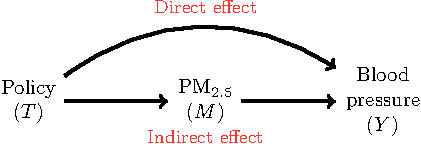
\includegraphics[width=0.6\textwidth,height=\textheight]{hei-report_files/figure-pdf/fig-dag1-1.pdf}

}

\caption{\label{fig-dag1}Hypothetical Directed Acyclic Graph showing
direct and indirect effects with outcome (\(Y\)), pre-treatment
covariates (\(X\)), policy (\(T\)), multiple mediators
(\(M_{1},M_{2}\)), as well as covariates for the mediators (\(W\)).}

\end{figure}

Although other mediated effects such as ``natural'' direct and indirect
effects are theoretically estimable (VanderWeele 2015), they involve
challenging ``cross-world'' assumptions that are difficult to anchor in
policy (Naimi et al. 2014). Other approaches to mechanisms have focused
on principal stratification (e.g., Zigler et al. 2016), although
conceptual difficulties with identifying the (unverifiable) principal
strata make it challenging for questions of mediation. Because
controlled direct effects are considered more directly policy relevant
for public health, we focus on estimating these mediated quantities.

\hypertarget{data-analysis}{%
\section{Data Analysis}\label{data-analysis}}

To understand how the policy's impact on health may be mediated by
different potential mediators, we need to estimate first the total
effect of the policy on the outcomes, as well as the \(CDE\)s with
adjustment for potential mediators. As discussed above, in order for the
mediators to `explain' the total effects of the policy on health, the
policy should affect the mediators, and the mediators should also affect
the outcomes.

\hypertarget{total-effect}{%
\subsection{Total Effect}\label{total-effect}}

To estimate the total effect of the policy we used a DiD analysis that
accommodates staggered treatment rollout. To allow for heterogeneity in
the context of staggered rollout we used `extended' two-way fixed
effects (ETWFE) models (Wooldridge 2021) to estimate the total effect of
the CBHP policy. The mean outcome (replaced by a suitable link function
\(g(\cdot)\) for binary or count outcomes) was defined using a set of
linear predictors:

\begin{equation}\protect\hypertarget{eq-etwfe}{}{Y_{ijt}=g(\mu_{ijt}) = \alpha + \sum_{r=q}^{T} \beta_{r} d_{r} + \sum_{s=r}^{T} \gamma_{s} fs_{t}+ \sum_{r=q}^{T} \sum_{s=r}^{T} \tau_{rt} (d_{r} \times fs_{t}) + \varepsilon_{ijt}}\label{eq-etwfe}\end{equation}

where \(Y_{ijt}\) is the outcome for individual \(i\) in village \(j\)
at time \(t\), \(d_{r}\) represent treatment cohort dummies, i.e., fixed
effects for cohorts of villages that were first exposed to the policy at
the same time \(q\) (e.g., in 2019, 2020, or 2021), \(fs_{t}\) are time
fixed effects corresponding to different winter data collection
campaigns (2018-19, 2019-20, or 2021-22), and \(\tau_{rt}\) are the
cohort-time \emph{ATTs}. The ETWFE and other approaches that allow for
several (potentially heterogenous) treatment effects may also be
averaged to provide a weighted \(ATT\). Several potential possibilities
are feasible, including weighting by treatment cohorts or time since
policy adoption (Goin and Riddell 2023).

\hypertarget{mediation-analysis}{%
\subsection{Mediation Analysis}\label{mediation-analysis}}

As noted above, with respect to the mediation analysis we are chiefly
interested in the \(CDE\), which can be derived by adding relevant
mediators \(M\) to this model. If we also allow for exposure-mediator
interaction and potentially allow for adjustment for confounders \(W\)
of the mediator-outcome effect, we can extend equation
Equation~\ref{eq-etwfe} as follows:

\begin{equation}\protect\hypertarget{eq-etwfem}{}{
\begin{aligned}
Y_{ijt}=g(\mu_{ijt}) = \alpha + \sum_{r=q}^{T} \beta_{r} d_{r} + \sum_{s=r}^{T} \gamma_{s} fs_{t}+ \sum_{r=q}^{T} \sum_{s=r}^{T} \tau_{rt} (d_{r} \times fs_{t}) \\ + \delta M_{it} + \sum_{r=q}^{T} \sum_{s=r}^{T} \eta_{rt} (d_{r} \times fs_{t} \times M_{it}) + \zeta \mathbf{W} + \varepsilon_{ijt}
\end{aligned}
}\label{eq-etwfem}\end{equation}

where now \(\delta\) is the conditional effect of the mediator \(M\) at
the reference level of the treatment (again, represented via the series
of group-time interaction terms), and the collection of \(\eta\) terms
are coefficients for the product terms allowing for mediator-treatment
interaction. Finally, \(\zeta\) is a vector of coefficients for the set
of confounders contained within \(\mathbf{W}\).

As noted above, in the staggered DiD framework that allows for
heterogeneity, we do not have a single treatment effect but a collection
of group-time treatment effects that may be averaged in different ways.
This extends to the estimation of the \(CDE\), in which case we will
also have several \(CDE\)s that can be averaged to make inferences about
the extent to which the policy's impact is mediated by
\emph{PM\textsubscript{2.5}}. Based on the setup in
Equation~\ref{eq-etwfem} the \(CDE\) is estimated as:
\(\delta + \eta_{rt}MT\). In the absence of interaction between the
exposure and the mediator (i.e., \(\eta_{rt}=0\)) the \(CDE\) will
simply be the estimated treatment effects
\(\sum_{r=q}^{T} \sum_{s=r}^{T} \tau_{rt}\), i.e., the effect of the
policy holding \(M\) constant. For a valid estimate of the \(CDE\) we
must account for confounding of the mediator-outcome effect, represented
by \(W\) in the equation above. Baseline measures of both the outcome
and the proposed mediators inherent in our DiD strategy will help to
reduce the potential for unmeasured confounding of the mediator-outcome
effect (Keele et al. 2015).

We limited the mediation analysis to health outcomes for which we
observed a total effect of the CBHP policy..

\hypertarget{identification-of-potential-confounders-and-model-covariates}{%
\subsection{Identification of potential confounders and model
covariates}\label{identification-of-potential-confounders-and-model-covariates}}

DiD is a strong analytical approach that already minimizes the risk of
confounding, where cohort-fixed effects control for measured and
unmeasured time-constant factors that may differ between treatment
cohorts (e.g., genetics, altitude), and time-fixed effects control for
secular trends that affect all treatment cohorts similarly over the
study period (e.g., background improvements in ambient air quality or
household transition to more efficient heating).

For models estimating the effect of the policy on health outcomes, we
used directed acyclic graphs (DAGs) to identify potential time-varying
causes of both treatment by the policy and our study outcome(s) that
could differ between treatment groups, and adjusted for those potential
confounders in the regression models. For the mediation analysis, we
identified potential mediator-outcome confounders using the same
approach. These variables were identified from the relevant
peer-reviewed literature and our team's substantive knowledge about the
CBHP policy. In the multivariable models, we also adjusted for strong
predictors of the outcome that were not affected by treatment, and thus
not confounders, to improve model precision. The covariates included in
each of the models for cardiovascular and respiratory health outcomes
are provided in the tables.

For air pollution outcomes, we considered the following covariates:
village population and total number of households in the village;
temperature, relative humidity, wind direction, wind speed, boundary
layer height; home area and home area heated; home insulation; smoking
status of participant and whether or not they lived with a smoker;
whether or not the household reported using wood (i.e., biomass) for
household energy activities, and if so, self-reported quantity of wood.
Potential non-linearity between continuous covariates and our study
outcomes were evaluated using cubic splines. Ultimately, the following
covariates were included in the final DiD models for outdoor, indoor,
and personal exposures to air pollution, based on whether measurable
changes in the covariate over time were observed. For the final adjusted
DiD model for personal exposure `mixed combustion' source contributions,
the following covariates were included: temperature (represented by a
spline with 2 degrees of freedom); participant smoking status; and
whether or not the household reported using biomass fuel. For the final
adjusted DiD model for outdoor (community) `mixed combustion' source
contributions, the following covariates were included: total number of
households in the village; village population; and ambient relative
humidity (represented by a spline with 2 degrees of freedom).

\hypertarget{results-1}{%
\section{Results}\label{results-1}}

We retained all 50 study villages during this four-year longitudinal
assessment of village treatment by the CBHP policy in Beijing, though we
were only able to visit 41 villages in winter 2020-21 (S3) and also were
limited to village and household-level measurements of air quality,
indoor temperature, and stove use in that campaign due to to the COVID
pandemic. By S2, S3, and S4 there were 10, 17, and 20 of the 50 villages
treated by the policy, respectively. Figure~\ref{fig-flowchart} shows
the participation of villages, households, and participants across the
four waves of data collection. We conducted measurements in over 1000
participants in each of the three measurement campaigns that included
individual-level measurements. In total, we enrolled 1432 participants
into the study, of which 630 (43\%) participated in all three campaigns,
443 (31\%) participated in two campaigns and 365 (25\%) participated in
a single campaign. We did not observe any notable differences in
demographic characteristics or health behaviors between participants who
contributed to a different number of campaigns
(Table~\ref{tbl-each-campaign}) or between participants in each of the
three campaigns with individual measurements
(Table~\ref{tbl-diff-campaign}).

\hypertarget{tbl-each-campaign}{}
\begin{table}
\caption{\label{tbl-each-campaign}Demographic and health characteristics of participants in each study
campaign. }\tabularnewline

\centering
\begin{tabular}{l>{\centering\arraybackslash}p{2.5cm}>{\centering\arraybackslash}p{2.5cm}>{\centering\arraybackslash}p{2.5cm}}
\toprule
\textbf{Characteristic} & \textbf{Campaign 1 (2018-19) N=1003} & \textbf{Campaign 2 (2019-20) N=1110} & \textbf{Campaign 4 (2021-22) N=1028}\\
\midrule
Female, n (\%) & 580 (57.8) & 653 (58.8) & 612 (59.5)\\
Current smoker, n (\%) & 257 (25.6) & 295 (26.6) & 265 (25.8)\\
Any smoke exposure, n (\%) & 788 (78.6) & 897 (80.8) & 843 (82)\\
Age in years, Mean (SD) & 60.7 (9.2) & 61.4 (9.1) & 63.1 (9)\\
BMI in kg/m\textsuperscript{2}, Mean (SD) & 26.1 (3.7) & 25.7 (3.5) & 26.1 (4)\\
Waist circumference in cm, Mean (SD) & 86.8 (10.2) & 87.4 (9.4) & 91.4 (10.7)\\
\bottomrule
\end{tabular}
\end{table}

\hypertarget{tbl-diff-campaign}{}
\begin{table}
\caption{\label{tbl-diff-campaign}Demographic and health characteristics of participants who contributed
to different numbers of campaigns. }\tabularnewline

\centering
\begin{tabular}{l>{\centering\arraybackslash}p{2.5cm}>{\centering\arraybackslash}p{2.5cm}>{\centering\arraybackslash}p{2.5cm}}
\toprule
\textbf{Characteristic} & \textbf{1 Campaign N=365} & \textbf{2 Campaigns N=443} & \textbf{3 Campaigns N=630}\\
\midrule
Female, n (\%) & 211 (57.8) & 253 (57.1) & 370 (58.7)\\
Current smoker, n (\%) & 110 (30.1) & 117 (26.4) & 161 (25.6)\\
Any smoke exposure, n (\%) & 288 (78.9) & 360 (81.3) & 498 (79)\\
Age in years, Mean (SD) & 59.9 (9.2) & 60.5 (8.8) & 61.3 (9.1)\\
BMI in kg/m\textsuperscript{2}, Mean (SD) & 26.3 (3.6) & 25.8 (3.5) & 26.1 (3.7)\\
Waist circumference in cm, Mean (SD) & 90.3 (9.8) & 86.5 (10) & 86.9 (10.4)\\
\bottomrule
\end{tabular}
\end{table}

Study flowchart

\begin{figure}[H]

{\centering 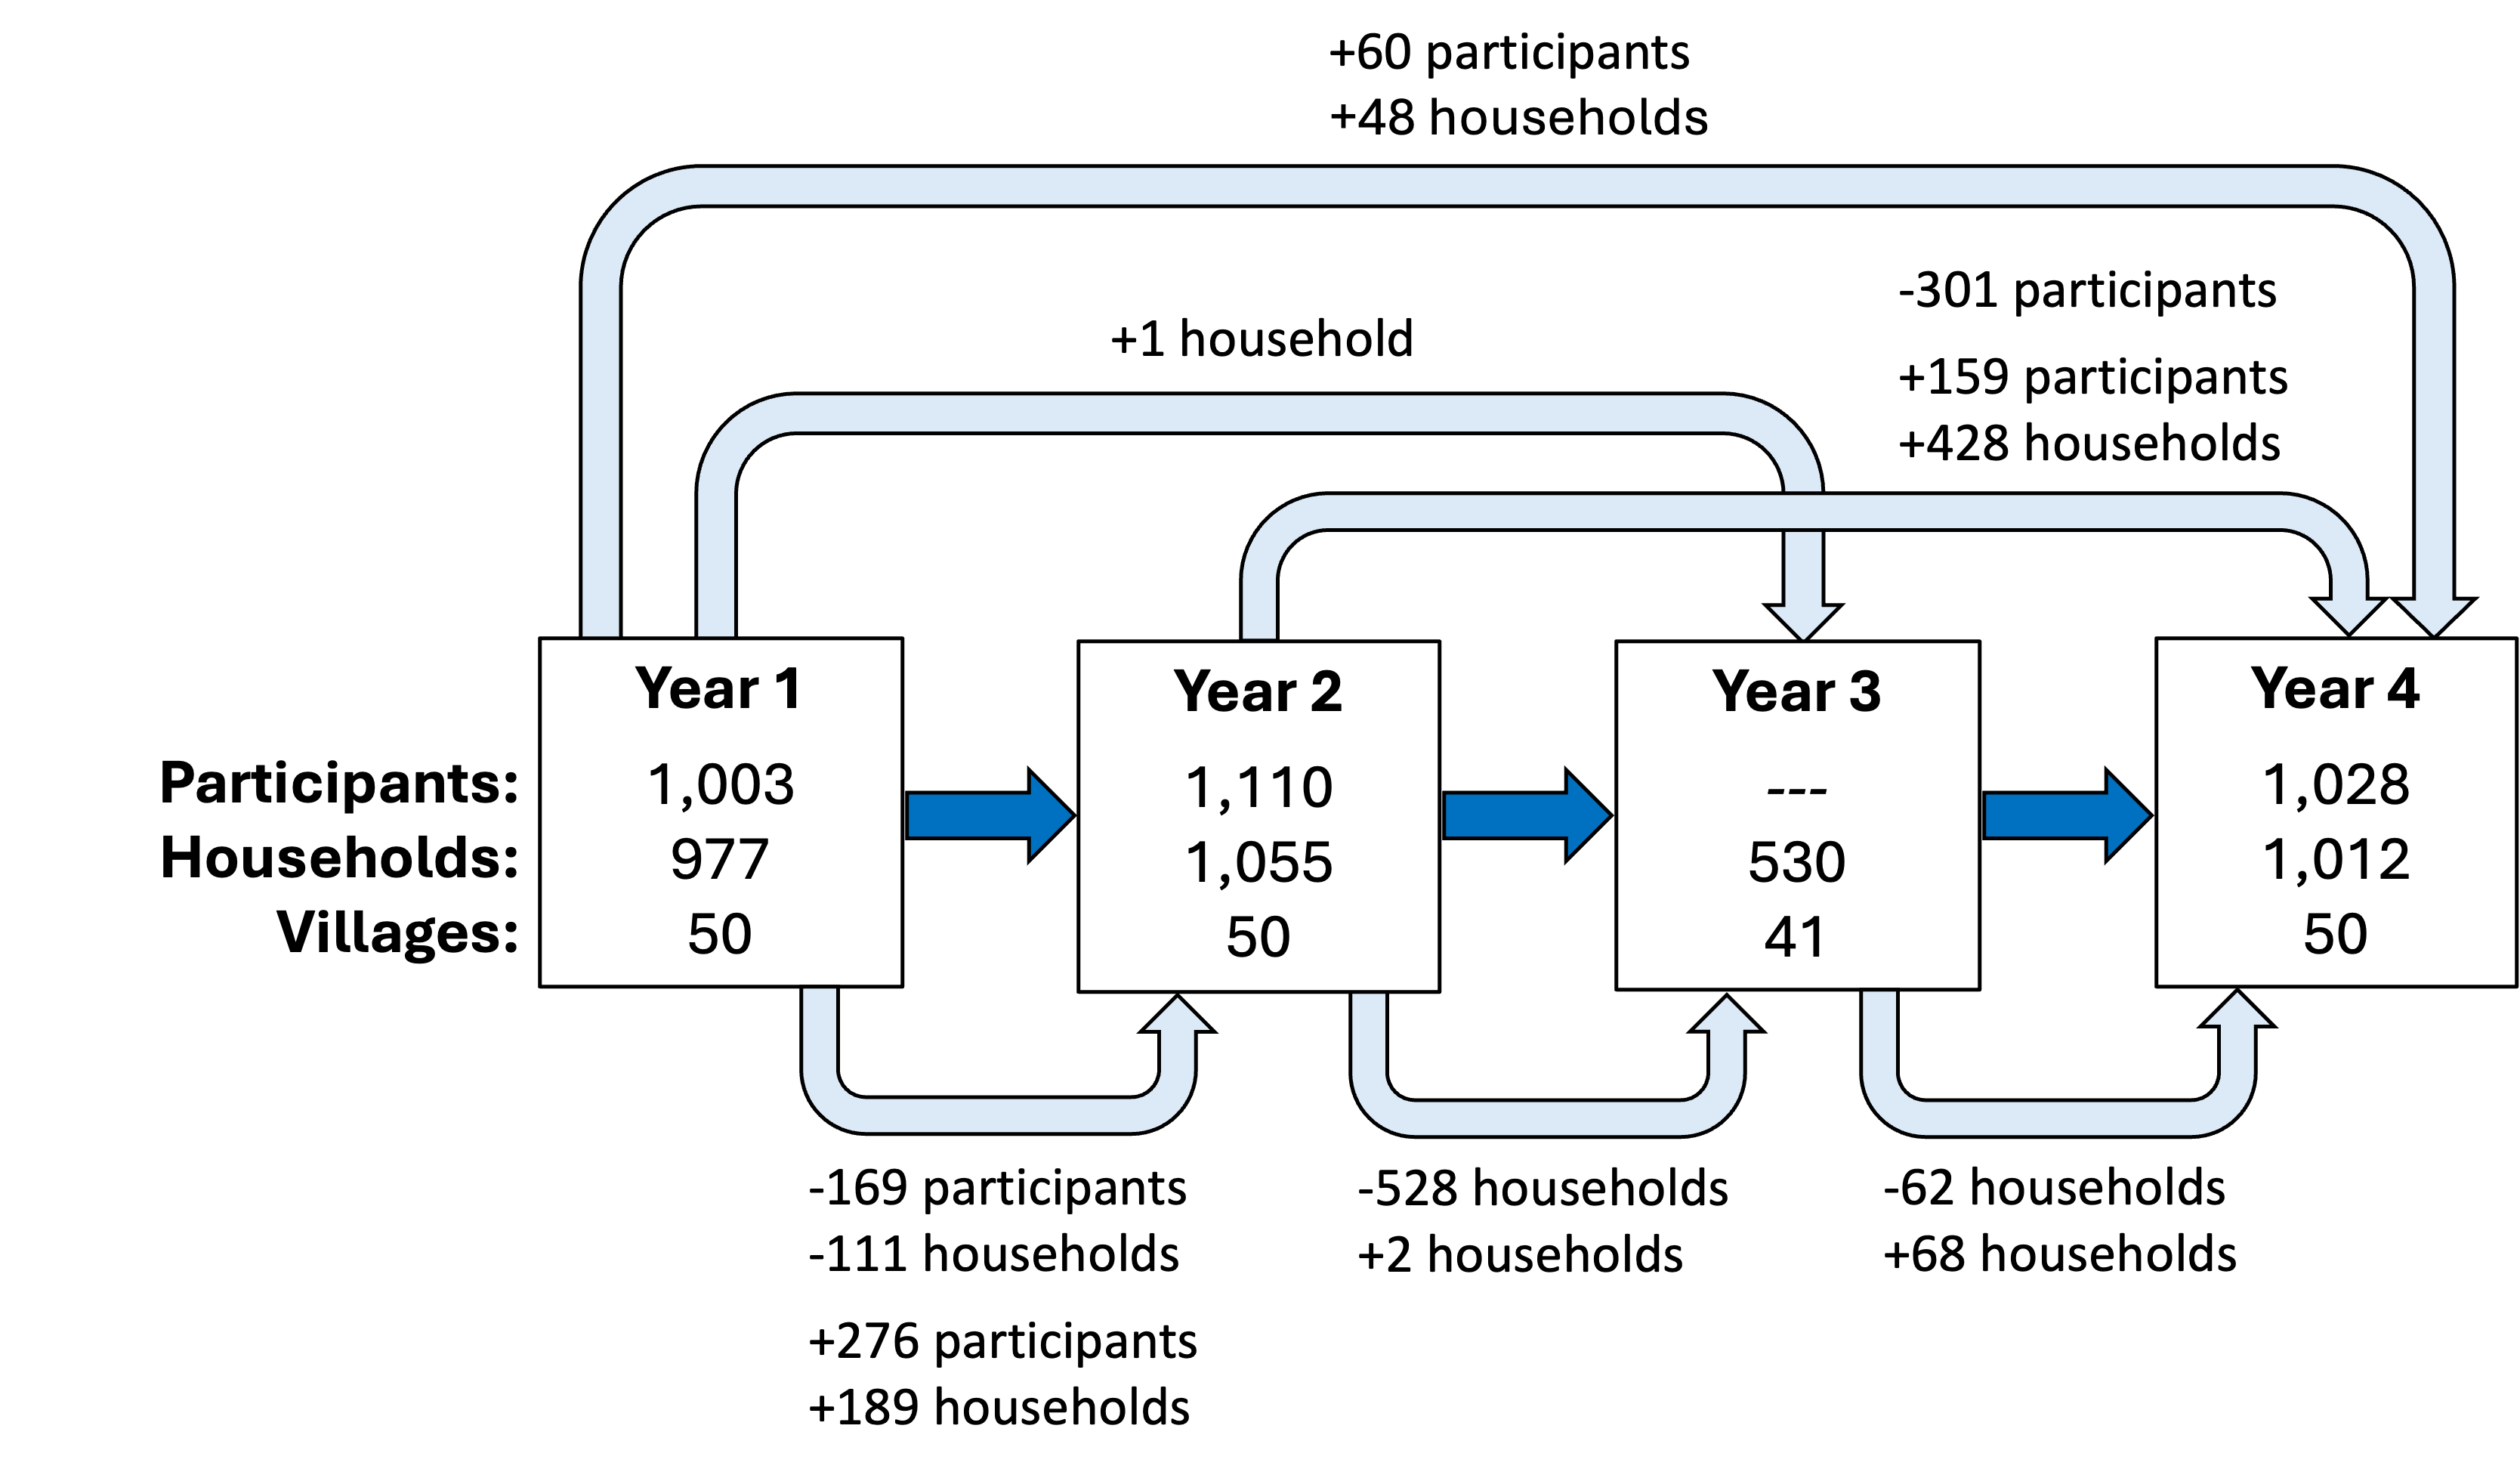
\includegraphics[width=0.8\textwidth,height=\textheight]{images/participation-flow-chart-Mar18.png}

}

\caption{\label{fig-flowchart}Flow chart of BHET study participation at
the participant, household, and village levels across study years.
Participation (number of units) in each study year is shown in the white
boxes. Additions (+) and losses (-) to the study sample between years
are indicated by the light blue arrows. Data collection was limited to
household- and village-level environmental measurements due to the
COVID-19 pandemic in year 3. We visited 530 households in 41 villages
before travel restrictions limited further data collection. This affects
the additions and losses to the study sample reported from years 2 to 3
and years 3 to 4.}

\end{figure}

\hypertarget{description-of-study-sample}{%
\subsection{Description of study
sample}\label{description-of-study-sample}}

\hypertarget{tbl-table1}{}
\begin{table}
\caption{\label{tbl-table1}Descriptive statistics for selected demographic, health, and
environmental measures at baseline, by treatment status }\tabularnewline

\centering\centering
\fontsize{9}{11}\selectfont
\begin{tabular}[t]{rrrrrrr}
\toprule
\multicolumn{1}{c}{ } & \multicolumn{2}{c}{Never treated (N=603)} & \multicolumn{2}{c}{Ever treated (N=400)} & \multicolumn{2}{c}{ } \\
\cmidrule(l{3pt}r{3pt}){2-3} \cmidrule(l{3pt}r{3pt}){4-5}
  & Mean & Std. Dev. & Mean & Std. Dev. & Diff. in Means & Std. Error\\
\midrule
\textbf{Demographics:} & \textbf{} & \textbf{} & \textbf{} & \textbf{} & \textbf{} & \textbf{}\\
Age (years) & 59.9 & 9.4 & 60.4 & 9.2 & 0.5 & 0.6\\
Female (\%) & 59.5 & 49.1 & 59.1 & 49.2 & -0.4 & 3.2\\
No education (\%) & 11.5 & 31.9 & 12.3 & 32.9 & 0.9 & 2.1\\
Primary education (\%) & 75.5 & 43.0 & 77.6 & 41.7 & 2.1 & 2.8\\
Secondary+ education (\%) & 12.6 & 33.2 & 9.8 & 29.7 & -2.9 & 2.0\\
\textbf{Health measures:} & \textbf{} & \textbf{} & \textbf{} & \textbf{} & \textbf{} & \textbf{}\\
Never smoker (\%) & 61.9 & 48.6 & 59.5 & 49.1 & -2.4 & 3.2\\
Former smoker (\%) & 11.9 & 32.4 & 15.1 & 35.8 & 3.2 & 2.2\\
Current smoker (\%) & 26.2 & 44.0 & 25.4 & 43.6 & -0.8 & 2.8\\
Never drinker (\%) & 55.9 & 49.7 & 52.5 & 50.0 & -3.4 & 3.2\\
Occasional drinker (\%) & 26.0 & 43.9 & 25.5 & 43.6 & -0.5 & 2.8\\
Daily drinker (\%) & 17.8 & 38.3 & 21.9 & 41.4 & 4.1 & 2.6\\
Systolic (mmHg) & 131.4 & 16.8 & 128.7 & 14.3 & -2.7 & 1.0\\
Diastolic (mmHg) & 82.7 & 11.6 & 82.1 & 11.3 & -0.6 & 0.8\\
Waist circumference (cm) & 87.7 & 10.5 & 85.4 & 9.5 & -2.3 & 0.8\\
Body mass index (kg/m2) & 26.3 & 3.7 & 25.8 & 3.6 & -0.5 & 0.3\\
Frequency of coughing (\%) & 18.7 & 39.0 & 19.7 & 39.8 & 1.0 & 2.6\\
Frequency of wheezing (\%) & 6.2 & 24.2 & 6.6 & 24.8 & 0.3 & 1.6\\
Shortness of breath (\%) & 29.2 & 45.5 & 34.3 & 47.5 & 5.1 & 3.0\\
Chest trouble (\%) & 11.6 & 32.0 & 14.1 & 34.9 & 2.5 & 2.2\\
Any respiratory problem (\%) & 50.6 & 50.0 & 54.3 & 49.9 & 3.7 & 3.2\\
\textbf{Environmental measures:} & \textbf{} & \textbf{} & \textbf{} & \textbf{} & \textbf{} & \textbf{}\\
Temperature (°C) & 13.8 & 3.6 & 13.5 & 3.3 & -0.3 & 0.2\\
Personal PM2.5 (ug/m3) & 150.2 & 300.3 & 103.8 & 107.3 & -46.3 & 19.1\\
\bottomrule
\end{tabular}
\end{table}

Table~\ref{tbl-table1} shows the distribution of selected demographic,
health, and environmental characteristics from the baseline survey,
prior to any villages being enrolled in the ban. We provide means and
standard deviations separately for villages that eventually enter into
the ban with those that never do so. As noted above, although our DiD
identification strategy allows for fixed differences between treated and
untreated villages, overall the differences at baseline are generally
small and the groups seem well balanced on most measures, with the
exception of personal PM\textsubscript{2.5} exposure, which was lower in
villages that were eventually treated.

Table~\ref{tbl-table1} shows the distribution of selected demographic,
health, and environmental characteristics from the baseline survey,
prior to any villages being enrolled in the CBHP policy. We provide
means and standard deviations separately for villages that eventually
enter into the ban with those that never do so. As noted above, although
our DiD identification strategy allows for fixed differences between
treated and untreated villages, overall the differences at baseline are
generally small and the groups seem well balanced on most measures, with
the exception of personal PM\textsubscript{2.5} exposure, which was
lower in villages that were eventually treated.

\hypertarget{summary-of-pm-and-bc-measurements}{%
\subsection{Summary of PM and BC
measurements}\label{summary-of-pm-and-bc-measurements}}

At baseline, fine particulate matter (PM\textsubscript{2.5}) and black
carbon (BC) concentrations were highest, on average, for personal
exposures compared with indoor and outdoor concentrations. From Season 2
onward, with the inclusion of indoor air pollution measurements,
personal exposure air pollution concentrations were still higher than
indoor or outdoor concentrations, with indoor levels being higher than
outdoors (Table~\ref{tbl-pm-season}). This trend (personal
\textgreater{} indoor \textgreater{} outdoor) was observed among
households in treated and untreated villages. Personal, indoor, and
outdoor geometric mean (95\% confidence interval) concentrations of
PM\textsubscript{2.5} were 72 (65,80), 45 (39,53), and 31 (28,35),
respectively, and elevated relative to health-based guidelines. The
current World Health Organization (WHO) guidelines state that annual
average concentrations of PM\textsubscript{2.5} should not exceed 5
µg/m3, while 24-hour average exposures should not exceed 15 µg/m3 for
more than 3 to 4 days per year (Organization 2021). Interim targets were
set to support the planning of incremental milestones toward cleaner
air, particularly for cities, regions, and countries with higher air
pollution levels. For PM\textsubscript{2.5}, the four interim (IT)
targets for annual and 24-h means are: IT-1: 35 and 75 µg/m3; IT-2: 25
and 50 µg/m3; IT-3: 15 and 37.5 µg/m3; and IT-4: 10 and 25 µg/m3
(Organization 2021). In our study, baseline personal exposures to
PM\textsubscript{2.5} fell between IT-1 and IT-2, indicating
considerable opportunity for air quality improvement from intervention.

\hypertarget{tbl-pm-season}{}
\begin{table}
\caption{\label{tbl-pm-season}Arithmetic and geometric means for air pollutant concentrations
(micrograms per cubic meter) by season. }\tabularnewline

\centering\begingroup\fontsize{9}{11}\selectfont

\begin{tabular}{lllcccccccc}
\toprule
\multicolumn{3}{c}{ } & \multicolumn{2}{c}{Season 1} & \multicolumn{2}{c}{Season 2} & \multicolumn{2}{c}{Season 3} & \multicolumn{2}{c}{Season 4} \\
\cmidrule(l{3pt}r{3pt}){4-5} \cmidrule(l{3pt}r{3pt}){6-7} \cmidrule(l{3pt}r{3pt}){8-9} \cmidrule(l{3pt}r{3pt}){10-11}
 &  &  & Est. & CI & Est. & CI & Est. & CI & Est. & CI\\
\midrule
\addlinespace[0.3em]
\multicolumn{11}{l}{\textbf{Personal}}\\
 &  & Mean & 117 & {}[105, 129] & 97 & {}[87, 107] &  &  & 84 & {}[72, 97]\\
\cmidrule{3-11}
 & \multirow[t]{-2}{*}{\raggedright\arraybackslash 24h PM2.5} & GM & 72 & {}[65, 80] & 59 & {}[53, 65] &  &  & 47 & {}[42, 52]\\
\cmidrule{2-11}
 &  & Mean & 4 & {}[3.5, 4.4] & 3.5 & {}[2.7, 4.2] &  &  & 3.7 & {}[2.9, 4.5]\\
\cmidrule{3-11}
\multirow[t]{-4}{*}[1\dimexpr\aboverulesep+\belowrulesep+\cmidrulewidth]{\raggedright\arraybackslash Filter-derived} & \multirow[t]{-2}{*}{\raggedright\arraybackslash 24h BC} & GM & 2.6 & {}[2.4, 2.8] & 1.9 & {}[1.7, 2.1] &  &  & 1.7 & {}[1.5, 1.9]\\
\cmidrule{1-11}
\addlinespace[0.3em]
\multicolumn{11}{l}{\textbf{Indoor}}\\
 &  & Mean &  &  & 94 & {}[84, 104] & 84 & {}[75, 94] & 67 & {}[60, 75]\\
\cmidrule{3-11}
\multirow[t]{-2}{*}{\raggedright\arraybackslash Sensor-derived} & \multirow[t]{-2}{*}{\raggedright\arraybackslash Seasonal PM2.5} & GM &  &  & 71 & {}[65, 78] & 63 & {}[57, 70] & 47 & {}[42, 52]\\
\cmidrule{1-11}
 &  & Mean &  &  & 69 & {}[59, 79] &  &  & 59 & {}[49, 69]\\
\cmidrule{3-11}
 & \multirow[t]{-2}{*}{\raggedright\arraybackslash 24h PM2.5} & GM &  &  & 45 & {}[39, 53] &  &  & 33 & {}[27, 40]\\
\cmidrule{2-11}
 &  & Mean &  &  & 2.3 & {}[1.8, 2.8] &  &  & 2.8 & {}[2.1, 3.4]\\
\cmidrule{3-11}
\multirow[t]{-4}{*}[1\dimexpr\aboverulesep+\belowrulesep+\cmidrulewidth]{\raggedright\arraybackslash Filter-derived} & \multirow[t]{-2}{*}{\raggedright\arraybackslash 24h BC} & GM &  &  & 1.6 & {}[1.3, 2.0] &  &  & 1.6 & {}[1.3, 1.9]\\
\cmidrule{1-11}
\addlinespace[0.3em]
\multicolumn{11}{l}{\textbf{Outdoor}}\\
 &  & Mean & 47 & {}[45, 48] & 55 & {}[54, 56] & 23 & {}[22, 23] & 33 & {}[32, 34]\\
\cmidrule{3-11}
\multirow[t]{-2}{*}{\raggedright\arraybackslash Sensor-derived} &  & GM & 36 & {}[35, 37] & 40 & {}[39, 41] & 33 & {}[32, 34] & 22 & {}[22, 23]\\
\cmidrule{1-1}
\cmidrule{3-11}
 &  & Mean & 38 & {}[34, 42] & 38 & {}[34, 41] &  &  & 26 & {}[24, 28]\\
\cmidrule{3-11}
 & \multirow[t]{-4}{*}{\raggedright\arraybackslash Seasonal PM2.5} & GM & 33 & {}[29, 36] & 30 & {}[28, 32] &  &  & 22 & {}[21, 24]\\
\cmidrule{2-11}
 &  & Mean & 1.5 & {}[1.3, 1.6] & 1.4 & {}[1.3, 1.5] &  &  & 1.2 & {}[1.1, 1.2]\\
\cmidrule{3-11}
\multirow[t]{-4}{*}[1\dimexpr\aboverulesep+\belowrulesep+\cmidrulewidth]{\raggedright\arraybackslash Filter-derived} & \multirow[t]{-2}{*}{\raggedright\arraybackslash Seasonal BC} & GM & 1.3 & {}[1.1, 1.4] & 1.1 & {}[1.0, 1.2] &  &  & 1 & {}[0.9, 1.1]\\
\bottomrule
\multicolumn{11}{l}{\rule{0pt}{1em}Note: Est. = Estimate, CI = 95\% CI, GM = Geometric Mean}\\
\end{tabular}
\endgroup{}
\end{table}

We also present the geometric and arithmetic means (and 95\% confidence
intervals) for PM\textsubscript{2.5} and BC in each seasonal measurement
campaign (Table~\ref{tbl-pm-season}). Season 3 (2020/2021) was a partial
campaign that took place over a time period impacted by the COVID-19
pandemic and did not involve filter-based air pollution sample
collection.

\hypertarget{policy-uptake}{%
\subsection{Policy uptake}\label{policy-uptake}}

Each year of the study, participants reported the types of fuels and
stoves and the amount of fuel used for space heating in winter. Based on
these data, heating energy types were classified into four categories:
exclusive use of a heat pump (`heat pump exclusively'), use of a heat
pump and a biomass-fueled kang (`heat pump with kang'), use of solid
fuel heater with an electric heating devices other than heat pumps
(`solid fuel with electricity (not heat pump)'), and exclusive use of
solid fuel. In villages treated by the policy, Figure~\ref{fig-sankey}
shows meaningful transitions from solid fuel to electric-powered heat
pumps for all treatment cohorts. For example, the proportion of
households in the group treated in S2 using heat pumps increased from
3\% in S1 to 93\% in S2 and 96\% in S4. Conversely, use of coal stoves
decreased from 97\% in S1 to 8\% in S2 and 3\% in S4. We observed
similar stove use transitions for households in villages treated in S3
and S4.

We also observed a substantial decline in the amount of self-reported
coal use when villages entered into the CBHP policy (Appendix
Figure~\ref{fig-afig-coal}). Reductions in coal use were consistent
across coal types, including both honeycomb briquettes (reported by
number of briquettes) and traditional coal (reported by the ton). At the
same time, participant-reported wintertime expenditures (reported in
Chinese Yuan) on electricity in each year of the study increased once
villages entered the CBHP policy. Biomass (i.e., wood logs/twigs or
charcoal) represents another source of heating fuel not expressly
targeted by the CBHP policy. In villages treated in S2 and S3, the use
of wood declined once villages entered the policy, but not to the same
degree as coal use declined. In villages treated in S4 -- albeit a small
number (n=3 villages) -- the use of wood showed a small increase after
treatment.

In untreated villages, an active transition from solid fuel to clean
energy was also observed during our four year study period. The
proportion of households using heat pumps increased gradually from 5\%
in S1 to 10\% in S2 and 25\% in S4. Commensurately, the reported
expenditures on electricity increased gradually over time in the
untreated villages (Appendix Figure~\ref{fig-afig-coal}). The percentage
of untreated households using solid fuel with electric devices remained
relatively stable, ranging from 64\% to 70\%. The use of wood fuel
remained stable, as well, at approximately one ton of fuel per winter.
However, exclusive use of solid fuel decreased from 30\% in S1 to 7\% in
S4.

\begin{figure}[H]

{\centering 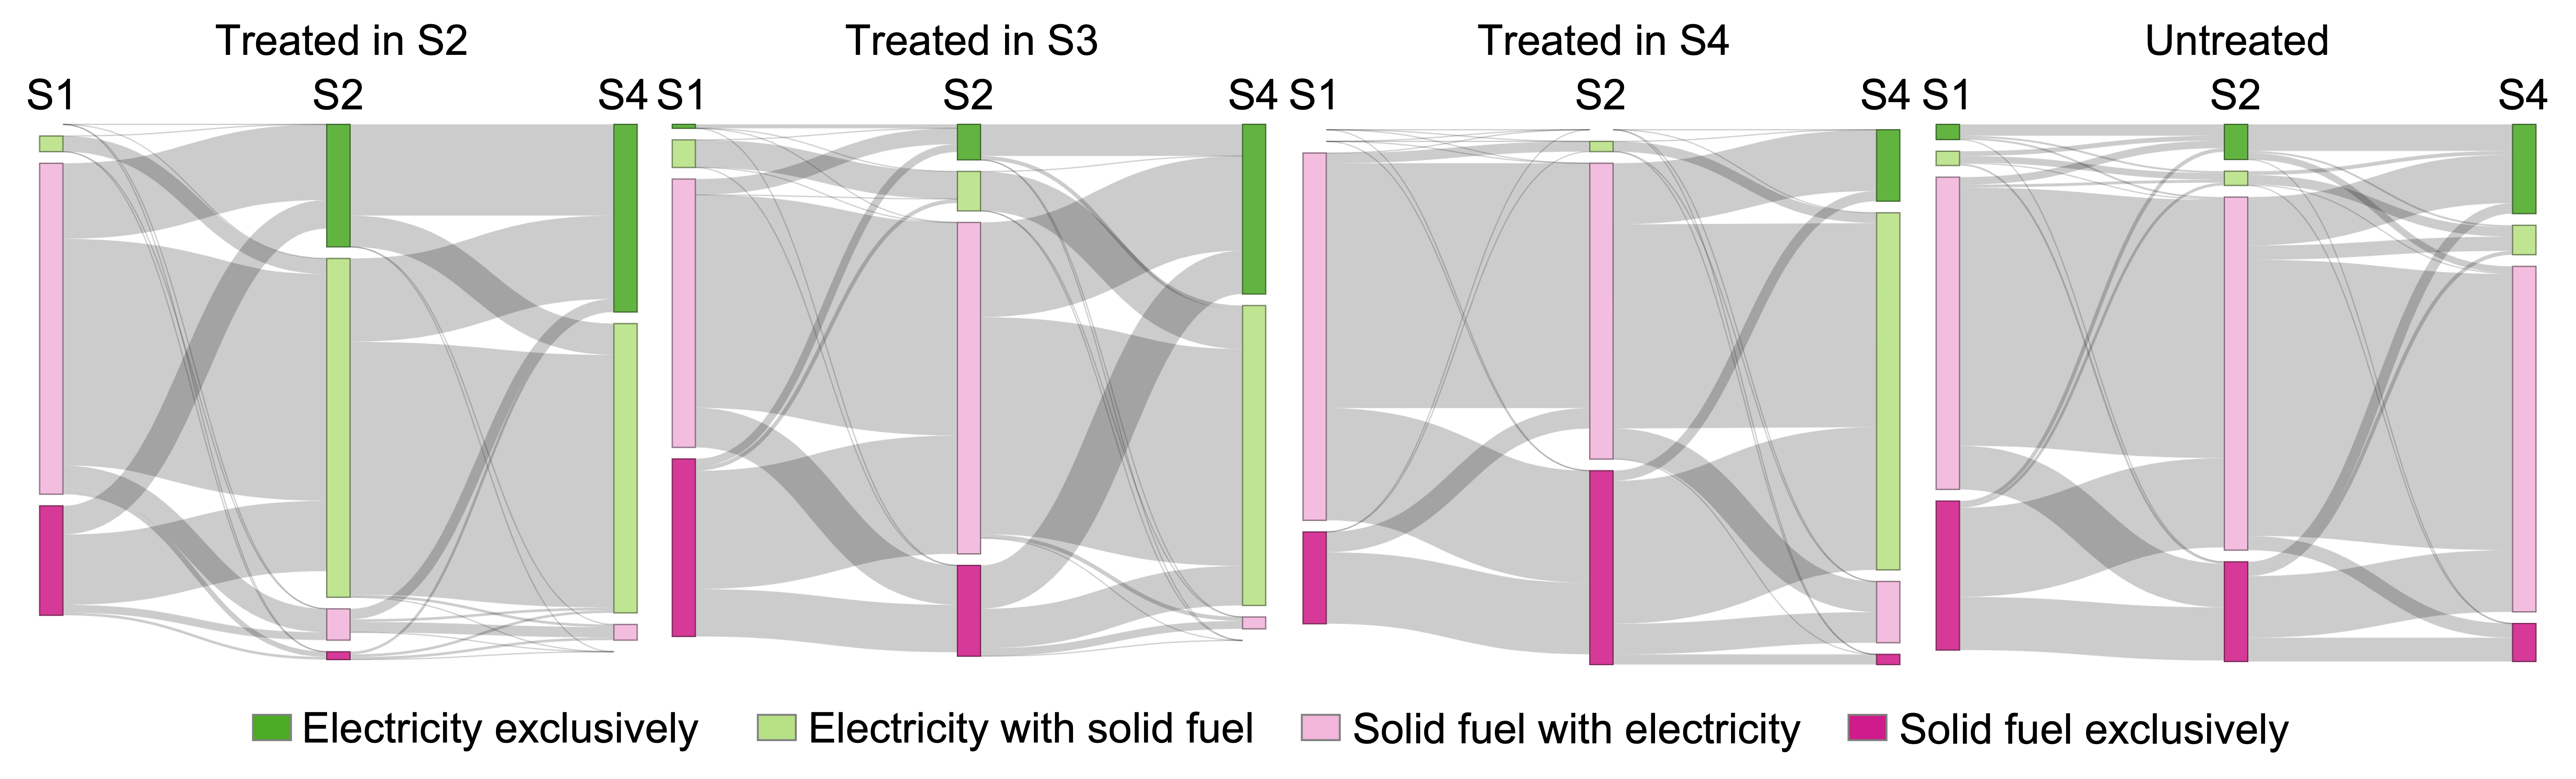
\includegraphics[width=1\textwidth,height=\textheight]{images/Sankey diagram_2.png}

}

\caption{\label{fig-sankey}Transitions to different energy sources
across study seasons}

\end{figure}

\hypertarget{aim-1-policy-impacts-and-potential-mediation}{%
\subsection{Aim 1: Policy impacts and potential
mediation}\label{aim-1-policy-impacts-and-potential-mediation}}

\hypertarget{impact-of-policy-on-potential-mediators}{%
\subsubsection{Impact of policy on potential
mediators}\label{impact-of-policy-on-potential-mediators}}

In estimating the treatment effect on indoor and outdoor air pollution,
we evaluated both 24-h mean values (specifically, the same 24-h period
when personal exposure samples were collected in each village) and
seasonal mean values (with `season' defined from Jan.~15th to Mar.~15th)
of PM\textsubscript{2.5} data collected in each village. For estimating
the treatment effect on personal exposure to PM\textsubscript{2.5} and
black carbon (BC), the results from the filter-based measurements that
were collected for a 24-h period were used for analysis. We estimated
the basic ETWFE models for outdoor, personal, and indoor measures of air
pollution. ETWFE models were further adjusted for covariates, including
temperature, relative humidity, wind speed, boundary layer height, wind
direction, and the mean quantity of wood burned in each village (for
outdoor measures of air pollution); outdoor temperature, dewpoint,
household smoking status, and the number of residents in each household
(for indoor measures of air pollution); and outdoor temperature,
dewpoint, household smoking status, and the number of residents in each
household (for personal measures of air pollution).

\hypertarget{tbl-did-med}{}
\begin{table}
\caption{\label{tbl-did-med}Treatment effect on outdoor and indoor PM\textsubscript{2.5}, as well as
personal exposure to PM\textsubscript{2.5} and black carbon. Outdoor and
indoor PM\textsubscript{2.5} were derived from sensor measurements after
being adjusted based on co-located gravimetric PM\textsubscript{2.5}
measurements. 24h indicates the mean PM\textsubscript{2.5}
concentrations during the 24 hours when personal exposure samples were
collected in each village. `Seasonal' indicates the seasonal mean
PM\textsubscript{2.5} concentrations in each village, from Jan. 15th to
Mar. 15th. }\tabularnewline

\centering
\begin{threeparttable}
\begin{tabular}{llcccc}
\toprule
\multicolumn{2}{c}{ } & \multicolumn{2}{c}{DiD} & \multicolumn{2}{c}{Adjusted DiD\textsuperscript{a}} \\
\cmidrule(l{3pt}r{3pt}){3-4} \cmidrule(l{3pt}r{3pt}){5-6}
  &   & ATT & (95\% CI) & ATT & (95\% CI)\\
\midrule
\addlinespace[0.3em]
\multicolumn{6}{l}{\textbf{Air pollution (µg/m\textsuperscript{3})}}\\
\hspace{1em} & PM2.5 & -2.09 & (-29.38, 25.2) & 1.95 & (-23.34, 27.23)\\
\cmidrule{2-6}
\multirow[t]{-2}{*}[1\dimexpr\aboverulesep+\belowrulesep+\cmidrulewidth]{\raggedright\arraybackslash Personal} & Black carbon & -0.46 & (-1.73, 0.81) & -0.43 & (-1.67, 0.81)\\
\cmidrule{1-6}
\hspace{1em} & Daily & -19.10 & (-60.56, 22.35) & -14.20 & (-53.94, 25.54)\\
\cmidrule{2-6}
\multirow[t]{-2}{*}[1\dimexpr\aboverulesep+\belowrulesep+\cmidrulewidth]{\raggedright\arraybackslash Indoor} & Seasonal & -35.11 & (-59.36, -10.85) & -36.19 & (-60.74, -11.65)\\
\cmidrule{1-6}
\hspace{1em} & Daily & -0.11 & (-5.86, 5.64) & -1.73 & (-9.26, 5.81)\\
\cmidrule{2-6}
\multirow[t]{-2}{*}[1\dimexpr\aboverulesep+\belowrulesep+\cmidrulewidth]{\raggedright\arraybackslash Outdoor} & Seasonal & 3.14 & (-3.1, 9.38) & 0.36 & (-6.27, 6.99)\\
\cmidrule{1-6}
\addlinespace[0.3em]
\multicolumn{6}{l}{\textbf{Indoor temperature (°C)}}\\
\hspace{1em}Point temp & Mean & 1.96 & (0.96, 2.96) & 1.96 & (0.96, 2.96)\\
\cmidrule{1-6}
\hspace{1em} & Mean (all) & 0.64 & (0, 1.29) & 0.64 & (0, 1.29)\\
\cmidrule{2-6}
\hspace{1em} & Mean (daytime) & 0.82 & (-0.08, 1.72) & 0.82 & (-0.08, 1.72)\\
\cmidrule{2-6}
\hspace{1em} & Mean (heating) & 1.80 & (0.96, 2.64) & 1.80 & (0.96, 2.64)\\
\cmidrule{2-6}
\hspace{1em} & Mean (daytime heating) & 1.85 & (0.97, 2.73) & 1.85 & (0.97, 2.73)\\
\cmidrule{2-6}
\hspace{1em} & Min. (all) & 3.83 & (2.26, 5.39) & 3.83 & (2.26, 5.39)\\
\cmidrule{2-6}
\multirow[t]{-6}{*}[5\dimexpr\aboverulesep+\belowrulesep+\cmidrulewidth]{\raggedright\arraybackslash Seasonal} & Min. (heating) & 3.72 & (2.19, 5.25) & 3.72 & (2.19, 5.25)\\
\bottomrule
\end{tabular}
\begin{tablenotes}
\item \small{Note: ATT = Average Treatment Effect on the Treated, DiD = Difference-in-Differences, ETWFE = Extended Two-Way Fixed Effects.}
\item[a] \small{ETWFE models for air pollution outcomes were adjusted for household size, smoking, outdoor temperature, and outdoor humidity. Temperature models not additionally adjusted.}
\end{tablenotes}
\end{threeparttable}
\end{table}

Treatment was associated with similar reductions in both seasonal and
24-h indoor PM\textsubscript{2.5} means (Table~\ref{tbl-did-med}). On
average, treatment was associated with a decrease in 24-h indoor
PM\textsubscript{2.5} of -38 µg/m\textsuperscript{3} {[}-75, -1{]}
μg/m3. After adjusting for covariates such as outdoor temperature,
dewpoint, household smoking status, and the number of residents in each
household, the treatment effect decreased to -31 {[}-64, -2{]} μg/m3.
The treatment effect on seasonal indoor PM2.5 (-39 {[}-55, -23{]} μg/m3)
remained consistent after covariate adjustment. This finding likely
reflects the direct benefit of the policy in replacing coal stoves,
thereby improving indoor air quality.

Overall we found little evidence of an impact of the CBHP policy on 24-h
and seasonal outdoor (local community-level) PM\textsubscript{2.5} or
personal exposures to PM\textsubscript{2.5} and BC. Treatment was
associated with lower, but statistically imprecise, personal 24-h BC
exposures. This finding would be consistent with the expectation that
the policy contributed to reducing air pollutant emissions from solid
fuel burning, as BC serves as a potential indicator of such combustion,
particularly in our study settings.

\hypertarget{impact-of-policy-on-health-outcomes}{%
\subsubsection{Impact of policy on health
outcomes}\label{impact-of-policy-on-health-outcomes}}

\hypertarget{tbl-did-health}{}
\begin{table}
\caption{\label{tbl-did-health}Overall impacts of the `coal-to-clean energy' policy on blood pressure,
respiratory outcomes, and inflammatory markers }\tabularnewline

\centering
\begin{threeparttable}
\begin{tabular}{llcccc}
\toprule
\multicolumn{2}{c}{ } & \multicolumn{2}{c}{DiD} & \multicolumn{2}{c}{Adjusted DiD\textsuperscript{a}} \\
\cmidrule(l{3pt}r{3pt}){3-4} \cmidrule(l{3pt}r{3pt}){5-6}
  &   & ATT & (95\% CI) & ATT & (95\% CI)\\
\midrule
\addlinespace[0.3em]
\multicolumn{6}{l}{\textbf{Blood pressure (mmHg)}}\\
\hspace{1em} & Brachial & -0.79 & (-2.63, 1.04) & -1.40 & (-3.31, 0.51)\\
\cmidrule{2-6}
\multirow[t]{-2}{*}[1\dimexpr\aboverulesep+\belowrulesep+\cmidrulewidth]{\raggedright\arraybackslash Systolic BP} & Central & -1.04 & (-2.82, 0.73) & -1.56 & (-3.40, 0.28)\\
\cmidrule{1-6}
\hspace{1em} & Brachial & -1.29 & (-2.62, 0.04) & -1.60 & (-2.96, -0.25)\\
\cmidrule{2-6}
\multirow[t]{-2}{*}[1\dimexpr\aboverulesep+\belowrulesep+\cmidrulewidth]{\raggedright\arraybackslash Diastolic BP} & Central & -1.35 & (-2.66, 0.04) & -1.66 & (-2.97, -0.34)\\
\cmidrule{1-6}
\hspace{1em} & Brachial & 0.50 & (-0.71, 1.70) & 0.21 & (-1.00, 1.41)\\
\cmidrule{2-6}
\multirow[t]{-2}{*}[1\dimexpr\aboverulesep+\belowrulesep+\cmidrulewidth]{\raggedright\arraybackslash Pulse Pressure} & Central & 0.31 & (-0.85, 1.46) & 0.10 & (-1.01, 1.20)\\
\cmidrule{1-6}
\hspace{1em} & Pulse pressure & 0.10 & (-0.12, 1.40) & 0.00 & (-1.20, 1.20)\\
\cmidrule{2-6}
\multirow[t]{-2}{*}[1\dimexpr\aboverulesep+\belowrulesep+\cmidrulewidth]{\raggedright\arraybackslash BP Amplification x10} & Systolic BP & 0.20 & (-0.20, 0.50) & 0.10 & (-0.20, 0.40)\\
\cmidrule{1-6}
\addlinespace[0.3em]
\multicolumn{6}{l}{\textbf{\makecell[l]{Respiratory\\outcomes}}}\\
\hspace{1em} & Any symptom & -7.38 & (-13.98, -0.77) & -7.86 & (-14.63, -1.09)\\
\cmidrule{2-6}
\hspace{1em} & Coughing & -1.59 & (-6.41, 3.23) & -1.98 & (-6.8, 2.84)\\
\cmidrule{2-6}
\hspace{1em} & Phlegm & -1.22 & (-5.58, 3.15) & -1.82 & (-6.34, 2.69)\\
\cmidrule{2-6}
\hspace{1em} & Wheezing attacks & -0.22 & (-3.97, 3.52) & -0.14 & (-3.85, 3.57)\\
\cmidrule{2-6}
\hspace{1em} & Trouble breathing & -4.98 & (-11.81, 1.84) & -4.62 & (-11.59, 2.35)\\
\cmidrule{2-6}
\multirow[t]{-6}{*}[5\dimexpr\aboverulesep+\belowrulesep+\cmidrulewidth]{\raggedright\arraybackslash Self-reported (pp)} & Chest trouble & -6.63 & (-12.51, -0.76) & -6.36 & (-12.14, -0.59)\\
\cmidrule{1-6}
\hspace{1em}Measured & FeNO (ppb) & 0.17 & (-2.24, 2.58) & 0.55 & (-2.13, 3.13)\\
\cmidrule{1-6}
\addlinespace[0.3em]
\multicolumn{6}{l}{\textbf{\makecell[l]{Inflammatory\\markers (\%)}}}\\
\hspace{1em} & IL6 & 6.80 & (-12.2, 30.0) & 5.90 & (-13.8, 30.2)\\
\cmidrule{2-6}
\hspace{1em} & TNF-alpha & 24.30 & (-1.3, 56.4) & 24.70 & (-0.9, 54.2)\\
\cmidrule{2-6}
\hspace{1em} & CRP & 2.70 & (-19.8, 31.6) & 3.80 & (-19.4, 33.6)\\
\cmidrule{2-6}
\multirow[t]{-4}{*}[3\dimexpr\aboverulesep+\belowrulesep+\cmidrulewidth]{\raggedright\arraybackslash } & MDA & 7.60 & (-8.7, 26.9) & 6.50 & (-9.7, 25.5)\\
\bottomrule
\end{tabular}
\begin{tablenotes}
\item \small{Note: ATT = Average Treatment Effect on the Treated, DiD = Difference-in-Differences, pp = percentage points, ppb = parts per billion.}
\item[a] \small{Blood pressure models adjusted for age, sex, waist circumference, smoking, alcohol consumption, and use of blood pressure medication.}
\end{tablenotes}
\end{threeparttable}
\end{table}

Table~\ref{tbl-did-health} shows the impacts of the policy on blood
pressure in basic ETWFE models and models further adjusted for age, sex,
waist circumference, smoking, alcohol consumption, and use of blood
pressure medication. Overall exposure to the CBHP policy demonstrated
reductions in blood pressure of approximately 1.5 mmHg for both systolic
and diastolic BP, but we found little evidence of a meaningful impact on
pulse pressure or BP amplification. The effects on brachial and central
blood pressures were similar.

Table~\ref{tbl-did-health} shows the impacts on self-reported chronic
respiratory symptoms categorized as any symptoms and separately for each
individual symptom type. In both basic and covariate-adjusted ETWFE
models, exposure to the CBHP policy reduced self-report of any poor
respiratory symptoms by around 7 percentage points. This was largely
through reductions in reports of having chest trouble or difficulty
breathing on several or most days of the week.

Table~\ref{tbl-did-health} shows the impacts of the CBHP on measured
airway inflammation (FeNO), which was conducted in a sub-sample of 511
participants, including 274 participants with one measurement, 142 with
two measurements, 95 participants with 3 measurements. We did not find
evidence that exposure to the policy affected changes in FeNO in the
covariate-adjusted ETWFE model (0.5 ppb, 95\%CI: -2.1, 3.1). There was
some evidence of heterogeneity in the FeNO effects of the policy by
treatment cohort, though the confidence intervals for each of the
cohort-specific effects were large and overlapping. Our results did not
change with sensitivity analyses that included a log-transformed FeNO
outcome and limiting the analysis to participants with at least two
repeated measurements and to those who participated in all three
campaigns (SI Table X)

\hypertarget{mediated-impact-on-blood-pressure}{%
\subsubsection{Mediated impact on blood
pressure}\label{mediated-impact-on-blood-pressure}}

As noted above, we aimed to assess whether any health impacts of the
CBHP policy may work specifically through pathways involving changes in
PM\textsubscript{2.5} and indoor temperature. Below we show results from
several mediation models. We evaluated potential mediation for each
mediator separately and in a single model accounting for multiple
mediators, and we set the values of both mediators to the WHO mean
annual interim PM\textsubscript{2.5} and indoor temperature guidelines.
For mediation analysis, we focused on BP outcomes for which we observed
an effect of the policy. In Table~\ref{tbl-bp-med} we show that
conditioning on indoor PM and indoor temperature largely explains the
entire total effect of the CBHP policy on blood pressure for systolic
BP, and roughly half of the total effect for diastolic BP.

\hypertarget{tbl-bp-med}{}
\begin{table}[H]
\caption{\label{tbl-bp-med}Controlled direct effects for the CBHP policy }\tabularnewline

\centering\begingroup\fontsize{10}{12}\selectfont

\begin{threeparttable}
\begin{tabular}{lcccccclc}
\toprule
\multicolumn{1}{c}{ } & \multicolumn{2}{c}{Adjusted Total Effect\textsuperscript{a}} & \multicolumn{6}{c}{CDE Mediated By:\textsuperscript{b}} \\
\cmidrule(l{3pt}r{3pt}){2-3} \cmidrule(l{3pt}r{3pt}){4-9}
\multicolumn{3}{c}{ } & \multicolumn{2}{c}{Indoor PM} & \multicolumn{2}{c}{Indoor Temp} & \multicolumn{2}{c}{PM + Temp} \\
\cmidrule(l{3pt}r{3pt}){4-5} \cmidrule(l{3pt}r{3pt}){6-7} \cmidrule(l{3pt}r{3pt}){8-9}
 & ATT & (95\%CI) & ATT & (95\%CI) & ATT & (95\%CI) & ATT & (95\%CI)\\
\midrule
Brachial SBP & -1.40 & (-3.31, 0.51) & -1.05 & (-3.12, 1.02) & -0.46 & (-2.29, 1.36) & -0.03 & (-2.04, 1.97)\\
Central SBP & -1.56 & (-3.40, 0.28) & -1.15 & (-3.20, 0.89) & -0.68 & (-2.36, 1.00) & -0.20 & (-2.11, 1.70)\\
Brachial DBP & -1.60 & (-2.96, -0.25) & -1.40 & (-2.97, 0.16) & -1.14 & (-2.33, 0.06) & -0.88 & (-2.30, 0.54)\\
Central DBP & -1.66 & (-2.97, -0.34) & -1.40 & (-2.96, 0.16) & -1.32 & (-2.50, -0.14) & -1.02 & (-2.45, 0.41)\\
\bottomrule
\end{tabular}
\begin{tablenotes}
\item \small{Note: Results combined across 30 multiply-imputed datasets. ATT = Average Treatment Effect on the Treated, CDE = Controlled Direct Effect, DBP = Diastolic blood pressure, SBP = Systolic blood pressure.}
\item[a] \small{Adjusted for age, sex, waist circumference, smoking, alcohol consumption, and use of blood pressure medication.}
\item[b] \small{Mediators were set to the mean value for untreated participants at baseline.}
\end{tablenotes}
\end{threeparttable}
\endgroup{}
\end{table}

\hypertarget{aim-2-source-contributions}{%
\subsection{Aim 2: Source
contributions}\label{aim-2-source-contributions}}

Source analysis for this study was conducted using data from all
eligible outdoor PM and personal PM samples. Eligible samples were those
for which PM\textsubscript{2.5} mass and chemical components were
quantified. We evaluated factors contributing to community-outdoor and
personal exposure PM\textsubscript{2.5} using the U.S. EPA's source
apportionment model PMF (positive matrix factorization) 5.0, which has
been widely used for similar analyses in China (Gao et al.~2018; Liu et
al.~2017; Tao et al.~2017). As an optimum PMF result depends on the
appropriate number of input factors, sensitivity analysis using a range
of factors (range of 3 to 7 factors, based on a combination of the
species that we have and our field-based observations and sources that
have been identified previously in our study region) were conducted to
examine the impact of a different number of factors on the model
results. Detailed information on the procedures of PMF analysis can be
found elsewhere (Wang et al.~2016; Zíková et al.~2016). Briefly, the
scree plot from our principal component analysis indicated that
solutions of between 3 and 5 factors (+/- 1) would be most appropriate,
further supporting our evaluation of 3 to 6 factor solutions from PMF.
There was no indication that even moving from five factors to six
factors would improve our solution; therefore, a seven factor solution
would not make sense to investigate further
(Figure~\ref{fig-source-figure}).

The chemical analysis data used as the input for the PMF model were
dispersion normalized prior to inclusion in the model. PMF works by
using covariance of compositional variables to separate sources of
ambient PM. However, atmospheric dilution also induces covariance.
Dilution can be quantified in terms of a ventilation coefficient (VC)
and used to normalize the input chemical concentrations and
uncertainties in the original data matrix on a sample by sample basis.
The dispersion normalized concentrations and uncertainties are used as
the input to PMF analysis. Dispersion normalization as conducted in this
study is a relatively new application of this conceptual framework (Dai
et al. 2020), developed to adjust for wind speed (dispersion in the x-y
plane) and boundary layer height (dispersion in the z-axis). This
process involves first calculating the sample specific ventilation
coefficient by multiplying the average wind speed by the average
boundary layer height over the sampling duration. The average
ventilation coefficient is also calculated for the village by averaging
all the ventilation coefficients. The dispersion normalized
concentration for any species in any sample is equal to the species
concentration in that sample multiplied by the ventilation coefficient
for that sample and divided by the average ventilation coefficient for
that village. Dividing by the average ventilation coefficient for that
village helps curtail any extreme concentrations driven by an outlier in
the sample ventilation coefficient.

The meteorological data included hourly boundary layer height, 2-m
temperature, 2-m dew point temperature, and 2-m horizontal wind speed
components (u, v), which were obtained from the European Center for
Midrange Weather Forecasting ERA5 reanalysis dataset (0.25 x 0.25
resolution). Values of these meteorological variables were determined at
the village-level by identifying the four surrounding grid points with
values available from the ERA5 reanalysis, and then applying inverse
distance weighted interpolation from those four grid points to the
village. Percent relative humidity was calculated from the 2-m dew point
temperature using the ``weathermetrics'' package (version 1.2.2) in R.
Total hourly wind speed and wind direction were calculated from the
horizontal wind speed components.

The model diagnostics for the three- to six-factor PMF solutions are
given in Table~\ref{tbl-pmf}. Model fit was assessed using Q/Qexp (how
our model fit divided by the expected fit). As the change in Q/Qexp
decreases as more factors are added, the model may be fitting additional
sources that do not improve the overall fit. The largest change in
Q/Qexp was from three to four sources (6.24 to 5.37) while the changes
moving from four to five and five to six are similar which suggests that
four factors is sufficient and parsimonious to explain the variation in
our data. We assessed the random error in our model by randomly sampling
blocks of data, fitting new models with the blocks, and comparing how
the source profiles compared to that of the original model (BS mapping).
The three- and four-factor solutions had high BS mapping (all factors
found in \textgreater{} 96.5\% of bootstrap runs). The additional
sources identified in the five-factor (lead) and six-factor (chloride)
solutions have low bootstrap mapping (\textgreater{} 72\%), which means
those solutions are not as consistent as the three- and four-factor
solutions. The possibility that multiple, different, solutions could
result in the same Q value was assessed using displacement. The
displacement approach takes the original factor profiles and modifies
the values for each species up or down to maintain a small change in Q,
reruns the solution with the new species values, and then compares the
profiles of the new model to the original. Any swaps indicate that small
changes in the species values could result in factor profiles that look
different from the original solution, and that the original solution is
unstable. None of the factors in any of the solutions discussed were
swapped during displacement, which indicates that all of the potential
solutions are stable. Based on the Q/Qexp, BS mapping, and
interpretability of the factors, the four-factor solution was selected
as the most appropriate source solution for the data.

\hypertarget{tbl-pmf}{}
\begin{table}
\caption{\label{tbl-pmf}PMF error estimation diagnostics }\tabularnewline

\centering\begingroup\fontsize{9}{11}\selectfont

\begin{tabular}{l>{\raggedright\arraybackslash}p{10em}>{\raggedright\arraybackslash}p{10em}>{\raggedright\arraybackslash}p{10em}>{\raggedright\arraybackslash}p{10em}}
\toprule
\multicolumn{1}{c}{ } & \multicolumn{4}{c}{Potential Factor Solution} \\
\cmidrule(l{3pt}r{3pt}){2-5}
Diagnostic & 3 & 4 & 5 & 6\\
\midrule
Qexp & 27936 & 26052 & 24168 & 22284\\
Qtrue & 187681 & 147796 & 123236 & 100316\\
Qrobust & 174407 & 139910 & 117082 & 95932.5\\
Qr/Qexp & 6.24 & 5.37 & 4.84 & 4.3\\
Q/Qexp > 6 & wi-Ca, ns-S, ws-Na, ws-Ca, Al, Cl, Pb & ns-S, Na, Al, Cl, Pb, Nitrate & Nitrate, ws-Na, Al, Chloride & Nitrate, ws-Na, Al\\
DISP \% dQ & <0.1\% & <0.1\% & <0.1\% & <0.1\%\\
DISP swaps & 0 & 0 & 0 & 0\\
BS\_mapping & Dust- 98.5\% & Transported dust- 95\%, Dust- 96.5\%, Sulfur secondary- 97.5\%, Mixed combustion- 96.5\% & Transported dust- 86\%, Mixed combustion- 87\%, Dust- 86\%, Lead- 55\% & Transported dust- 84\%, Mixed combustion- 87.5\%, Dust- 81.5\%, Lead- 72\%
Chloride- 61.5\%
Sulfur secondary- 98.5\%\\
\bottomrule
\end{tabular}
\endgroup{}
\end{table}

The source profiles for the four-factor solution are presented in
Figure~\ref{fig-source-figure}. The first source was identified as dust
by high percentages of crustal elements like wi-Ca, Si, and wi-Mg. The
second source consisted of non-sulfate sulfur as well as secondary
inorganic ions (ammonium, nitrate, and sulfate). Non-sulfate sulfur is a
tracer for primary coal combustion, while secondary inorganic ions
indicate a secondary source. Since industrial coal burning is a source
of power generation in our study area, it is likely that the second
source is a mixture of primary and secondary emissions that originate
from coal and other sulfurous fuel combustion. Additionally, the mean
source contribution of the second source is higher in outdoor than
personal exposure measurements. Secondary formation occurs outdoors in
the presence of sunlight, so higher outdoor concentrations compared to
personal exposure further support our naming the second source `sulfur
secondary'. The third source had high percentages of ws-Ca nd Al, which
in our study region, has been found to be indicative of transported dust
from dust storms that can occur in the spring. While our samples were
collected during winter months only, it is possible that transported
dust from previous years still remained. The fourth source was
characterized by high percentages of tracers for both coal (OC, wi-K,
chloride, Pb) and biomass combustion (EC, ws-K). Coal and biomass
combustion are anticipated sources of PM pollution in our study setting,
particularly from domestic cooking and heating activities, so this
source is likely a mixture of PM emitted from these two combustion
sources.

\begin{figure}[H]

{\centering 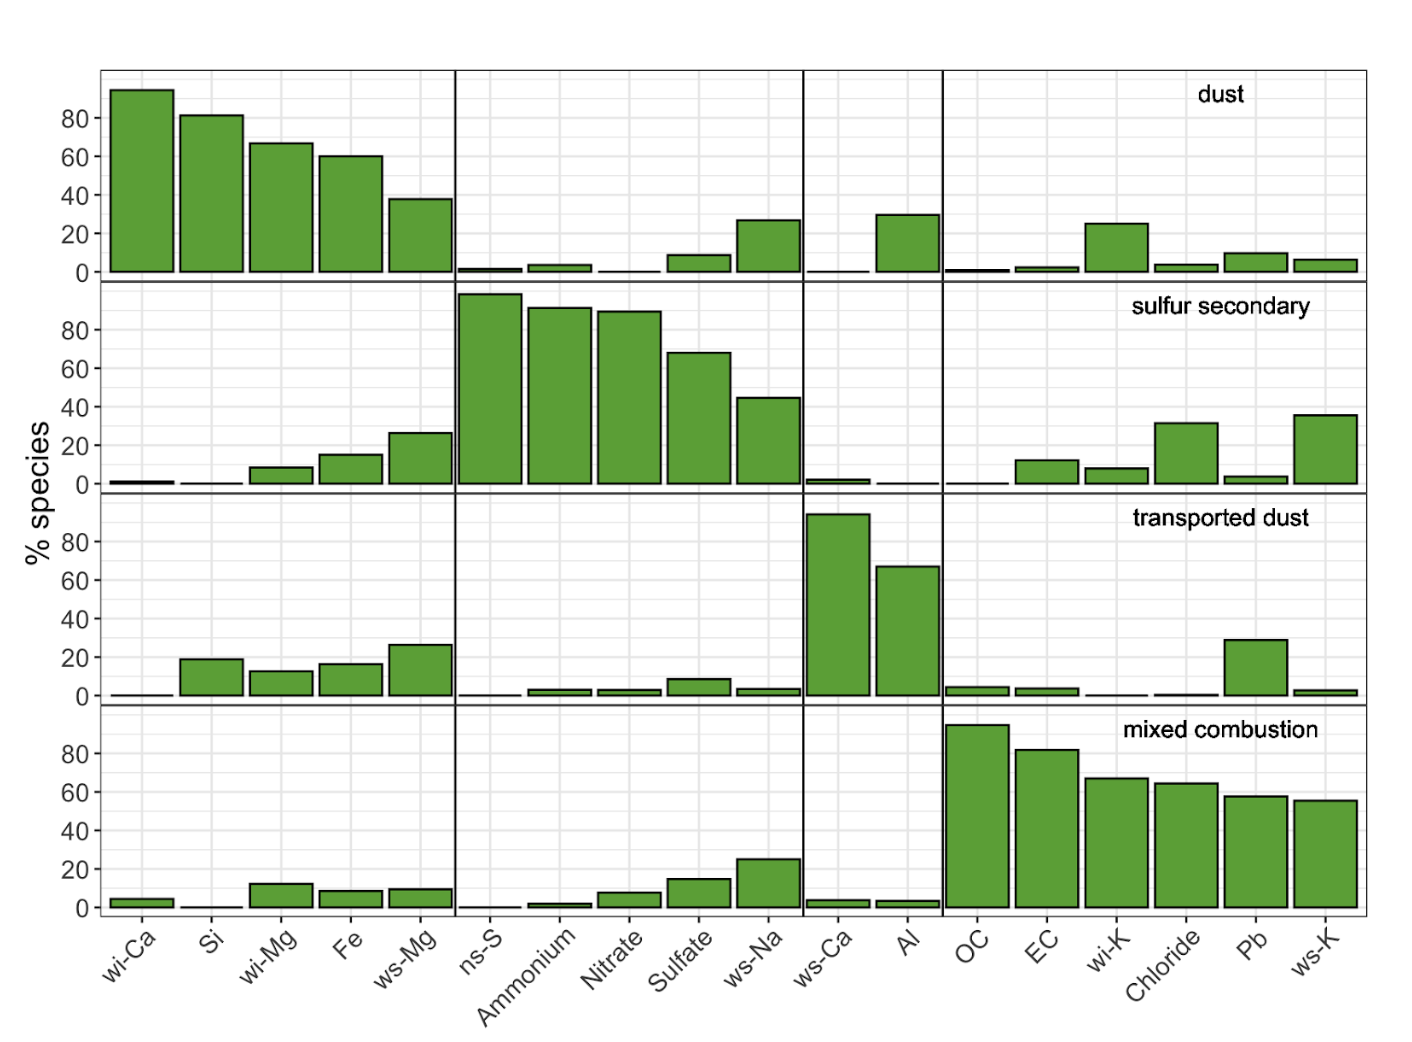
\includegraphics[width=0.8\textwidth,height=\textheight]{images/source-figure.png}

}

\caption{\label{fig-source-figure}Source profiles for the 4-factor PMF
solution to the sum of elements, ions, elemental carbon, and organic
carbon for outdoor and personal PM\textsubscript{2.5} exposure
measurements. The lines separate the major contributing species to each
source}

\end{figure}

We extend the source profiles across the different treatment cohorts in
Figure~\ref{fig-source-season}.

\begin{figure}[H]

{\centering 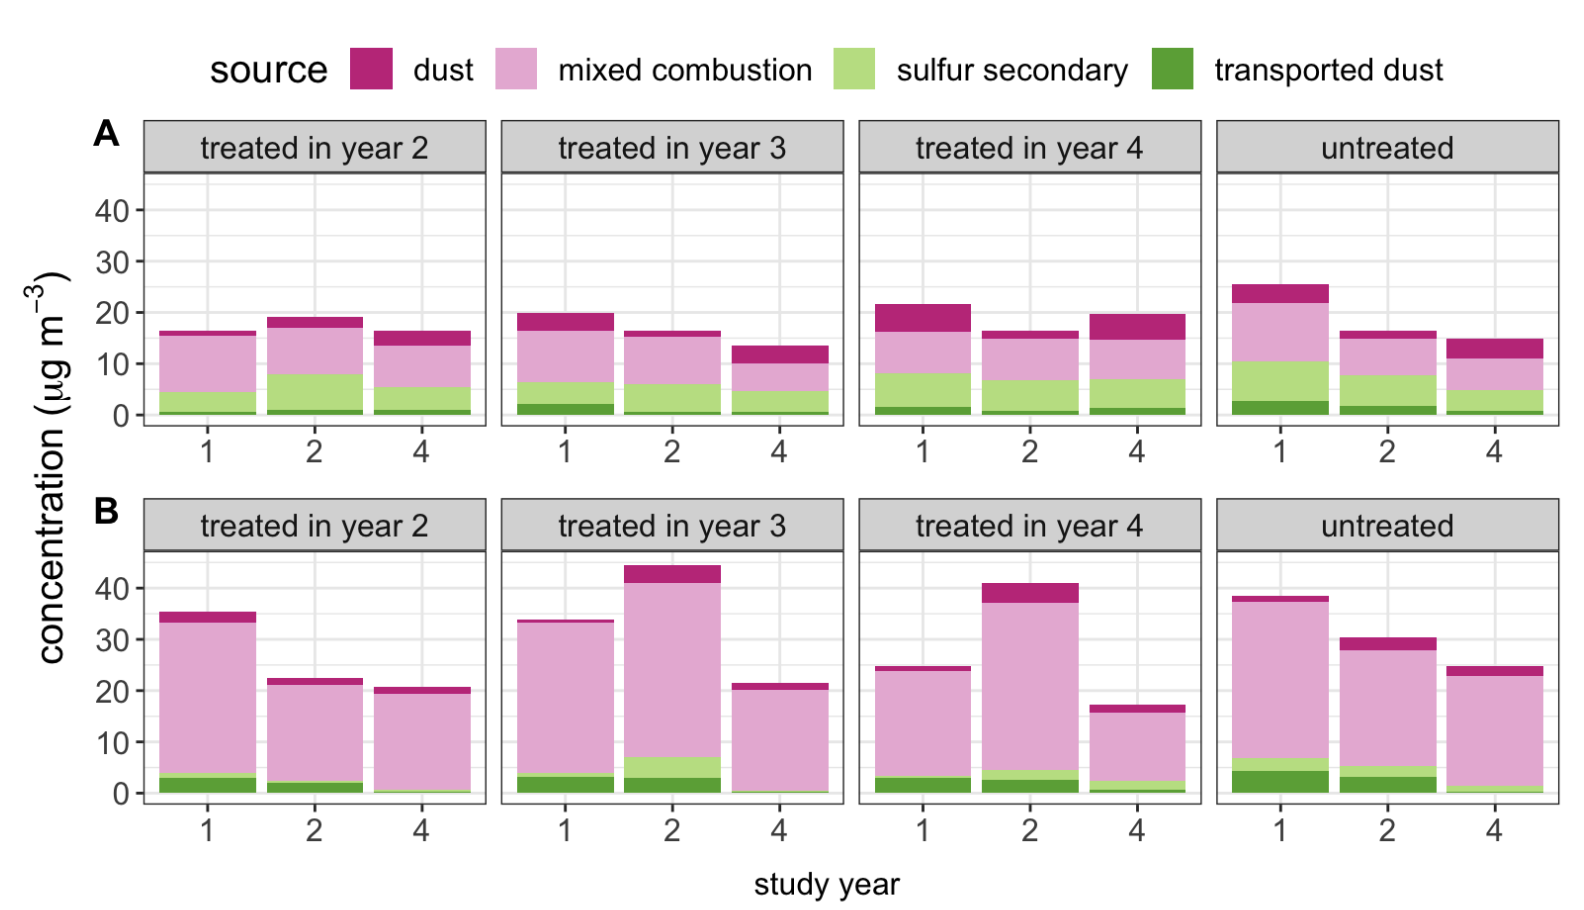
\includegraphics[width=0.8\textwidth,height=\textheight]{images/source-season.png}

}

\caption{\label{fig-source-season}Arithmetic mean dispersion normalized
source contributions found from the 4-factor PMF solution for A outdoor
and B personal PM\textsubscript{2.5} exposure samples by year the group
received treatment.}

\end{figure}

Overall, Table~\ref{tbl-source-did} shows the average treatment effect
of the CBHP policy on outdoor (community-level) and personal exposure to
the mixed combustion source was statistically indistinguishable from the
null. Treatment was associated with lower, but statistically imprecise,
personal exposures to the mixed combustion source. As with BC, this
finding is consistent with the expectation that the policy contributed
to reducing air pollutant emissions from solid fuel burning, as this
`mixed combustion' source most likely reflects solid fuel combustion,
particularly in our study settings. The results were consistent in the
unadjusted and adjusted models.

\hypertarget{tbl-source-did}{}
\begin{table}
\caption{\label{tbl-source-did}Average treatment effect (µg/m\textsuperscript{3}) for outdoor and
personal exposure to the mixed combustion source. }\tabularnewline

\centering
\begin{tabular}{lcccc}
\toprule
\multicolumn{1}{c}{ } & \multicolumn{2}{c}{DiD} & \multicolumn{2}{c}{Adjusted DiD\textsuperscript{a}} \\
\cmidrule(l{3pt}r{3pt}){2-3} \cmidrule(l{3pt}r{3pt}){4-5}
  & ATT & (95\% CI) & ATT & (95\% CI)\\
\midrule
Outdoor & 1.07 & (-4.90, 7.04) & 1.53 & (-4.19, 7.26)\\
Personal exposure & -5.60 & (-13.70, 2.54) & -5.39 & (-13.1, 2.35)\\
\bottomrule
\multicolumn{5}{l}{\rule{0pt}{1em}\textsuperscript{a} \small{Note: Models adjusted for ???}}\\
\end{tabular}
\end{table}

Figure X. Average treatment effect for outdoor and personal exposure to
the mixed combustion source.

Table X. Average treatment effect for outdoor and personal exposure to
the mixed combustion source.

{[}\ldots to be updated by Sam\ldots{]}

When the average treatment effect of the CBHP policy on outdoor
(community-level) and personal exposure to the mixed combustion source
was subset by treatment year (i.e., the DiD and adjusted DiD models were
evaluated separately for households treated in either Season 2, Season
3, or Season 4), the treatment effect for households most recently
treated (i.e., treated in the final season, Season 4) was associated
with lower personal exposures to the mixed combustion source. In each
season, treatment by the CBHP policy was associated with a reduction in
the source contribution to personal PM\textsubscript{2.5} mass from the
mixed combustion source; however, for villages treated in Seasons 2 and
3, the effect was statistically imprecise. Treatment was not associated
with a reduction or an increase in the source contribution to community
outdoor PM\textsubscript{2.5} mass from the mixed combustion source.
That personal exposure measures of this specific air pollution source
were more indicative of treatment effect than community outdoor measures
of the same air pollution source is consistent with the expectation that
this source is most characteristic of household use of solid fuels,
including coal and biomass, which would produce emissions that are
likely to be nearer to the people using those fuels than near to the
centrally located community outdoor air samplers.

Figure X. Adjusted and unadjusted treatment effect for outdoor and
personal exposure to the mixed combustion source by treatment year.

\hypertarget{aim-3}{%
\subsection{Aim 3}\label{aim-3}}

\begin{itemize}
\tightlist
\item
  Table of mediated health effects by source contribution (coal and
  biomass)
\end{itemize}

\hypertarget{tbl-med-source}{}
\begin{table}
\caption{\label{tbl-med-source}Average treatment effects and controlled direct effect (mm/Hg) of the
CBHP policy on central systolic and diastolic blood pressure with mixed
combustion source as the potential mediator. }\tabularnewline

\centering
\begin{threeparttable}
\begin{tabular}{lcccccc}
\toprule
\multicolumn{1}{c}{ } & \multicolumn{2}{c}{DiD} & \multicolumn{2}{c}{Adjusted DiD\textsuperscript{a}} & \multicolumn{2}{c}{Adjusted CDE\textsuperscript{b}} \\
\cmidrule(l{3pt}r{3pt}){2-3} \cmidrule(l{3pt}r{3pt}){4-5} \cmidrule(l{3pt}r{3pt}){6-7}
 & ATT & (95\%CI) & ATT & (95\%CI) & ATT & (95\%CI)\\
\midrule
Central SBP & -0.43 & (-3.48, 2.62) & -1.61 & (-5.03, 1.82) & -1.5 & (-4.94, 1.94)\\
Central DBP & -0.58 & (-2.59, 1.43) & -1.26 & (-3.38, 0.87) & -1.37 & (-3.69, 0.96)\\
\bottomrule
\end{tabular}
\begin{tablenotes}
\item \small{Note: ATT = Average Treatment Effect on the Treated, DiD = Difference-in-Differences, CDE = Controlled Direct Effect, DBP = Diastolic Blood Pressure, SBP = Systolic Blood Pressure.}
\item[a] \small{Adjusted for age, sex, waist circumference, smoking, alcohol consumption, and use of blood pressure medication.}
\item[b] \small{Further adjusted for mediation by mixed combustion source (coal and biomass)}
\end{tablenotes}
\end{threeparttable}
\end{table}

\hypertarget{discussion-and-conclusions}{%
\section{Discussion and Conclusions}\label{discussion-and-conclusions}}

Air pollution emitted from residential space heating with coal has
historically been a major contributor to cardio-respiratory disease
burden in northern China (Archer-Nicholls et al. 2016; Yun et al. 2020).
Since the introduction of its 13th 5-Year-Plan (2016-2020), China has
successfully implemented numerous large-scale measures to improve air
quality including programs that incentivize rural household transition
from solid fuels to clean energy sources (Young et al. 2015). The CBHP
policy is among the largest and most ambitious household energy policies
implemented anywhere in the world in recent decades, and its staggered
roll-out provided us with a unique opportunity to prospectively evaluate
its effects on air pollution levels and sources, indoor temperature, and
both cardiovascular and respiratory outcomes to understand how this
village-level energy intervention impacts health.

\hypertarget{adoption-of-the-heat-pump-technology-and-adherence-to-the-policy}{%
\subsection{Adoption of the heat pump technology and adherence to the
policy}\label{adoption-of-the-heat-pump-technology-and-adherence-to-the-policy}}

We observed high uptake and consistent use of the new heat pump
technology and large reductions in coal use in villages exposed to the
CBHP policy starting in the first year post-treatment and continuing
into the third year for villages treated in 2019 in our study. We
enrolled rural and peri-urban villages across a wide geographic area and
socioeconomic spectrum in Beijing and observed near universal adoption
of the heat pump technologies (93-96\% of households) and near universal
suspension of coal stove use in treated villages across the different
post-treatment campaigns. This contrasts with many previous household
energy intervention studies, including several randomized trials, where
low fidelity and compliance with the intervention limited its air
quality or health benefits (Ezzati and Baumgartner 2017; Harrison et al.
Approved February 2024; Rosenthal et al. 2018).

There are a number of possible reasons why uptake of the new technology
and adherence to the policy was so successful. The initial uptake of the
heat pump was likely influenced by broad support and perceived benefits
of the technology and participation in the policy. At baseline
assessment, 49 of 50 village committee interviewees indicated a desire
to participate in policy by the committee members and their
constituents, for reasons including convenience (i.e., no need to add
briquettes to the stove during night), clean environment, and no risk of
carbon monoxide poisoning. In addition, several other factors also
contribute to the high compliance rate in the treated villages. First,
households in the treated village do not have access to briquettes.
Currently, the procurement and distribution of briquettes for winter
home heating in rural areas of Beijing is centralized by district
governments. Prior to each heating season, village committees that have
not yet implemented the ``coal to electricity'' program collect orders
from households for briquettes and submit them to the district
government. The district government selects suppliers for centralized
procurement and distribution through a bidding process. Therefore, once
a village joins the ``coal to electricity'' program, the village
committee will no longer be able to order briquettes.

Secondly, strict environmental inspections and enforcement measures play
a crucial role. Most villages in Beijing are equipped with air pollution
detection equipment. When the Environmental Protection Department
identifies serious air pollution within a village, it holds the village
committee leaders accountable. Consequently, the leaders of the treated
villages are incentivized to prevent residents from burning coal.
Additionally, the Environmental Protection Department conducts
inspections and issues warnings regarding coal re-burning. If a
household in a treated village is found engaging in coal re-burning,
they face the risk of losing the clean heating subsidy.

Availability and cost of clean fuel and the upfront and repair costs of
new cookstoves have also been barriers to the continued use of new
cookstoves over time (Rehfuess et al. 2014). In our study, both the
upfront costs of the heat pump and electricity were highly subsidized by
the government, which limited the financial burden of transition for
households. Most previous studies evaluated cookstove interventions
which often required behavioral change in preparing fuel or cooking
food, whereas use of the heat pumps required relatively minimal
behavioral change since the technology is easy to operate.

\hypertarget{impacts-of-the-policy-on-health}{%
\subsection{Impacts of the policy on
health}\label{impacts-of-the-policy-on-health}}

One of the key findings from our comprehensive evaluation of the CBHP
policy was that exposure to the policy reduced systolic and diastolic
blood pressure by \textasciitilde1.5 mmHg, and that most of the observed
BP benefits were mediated by improvement in the indoor environment,
specifically reductions in indoor PM\textsubscript{2.5} and increases in
indoor temperature. The findings are supported by a small number of
randomized and non-randomized intervention studies (with pre-post
measured and control groups) of gas or more efficient biomass cookstoves
showing similar or larger reductions in blood pressure (SBP range: XXX
mmHg; DBP range: \#\#\# mmHg) (Kumar et al. 2021). In contrast, a
previous energy program assessment in southern China observed small
increases in BP (\textasciitilde1.3 mmHg) among women who received a
semi-gasifier cookstove and pelletized biomass fuel. In that study,
exposure to air pollution and BP decreased in both intervention and
control households but the reductions were larger controls
(PM\textsubscript{2.5}: 48−70\% lower; SBP: -4.1 mmHg) than the
intervention group (PM\textsubscript{2.5}: 24−67\% lower; SBP: -2.7
mmHg), a result likely driven by an unexpected shift to gas stoves in
control households (Clark et al. 2019). Similarly, a recent
multi-country randomized trial observed a small increase in gestational
blood pressure in pregnant women who received gas stoves (Ye et al.
2022) despite decreases in exposure to PM\textsubscript{2.5} larger than
those observed in our study, though the gas stoves can still emit
health-damaging air pollutants like benzine and volatile organic
compounds (Kashtan et al. 2023), especially in contrast to the
zero-emission electric heaters introduced in our study villages through
the CBHP policy.

Our findings of temperature- and air quality-mediated impacts of the
policy on BP are supported by observational studies conducted by us and
others showing that increased exposures to household air pollution
(Baumgartner et al. 2018, 2011; Dong et al. 2013; Kanagasabai et al.
2022) and to colder indoor temperatures (Lv et al. 2022; Sternbach et
al. 2022) are associated with higher blood pressure in rural and
peri-urban areas of China, with exposure-response estimates that align
with our mediator estimates. For example, {[}{[}{[}give some examples
here to contextualize and compare{]}{]}{]}

We did not observe effects of the policy on blood pressure measures of
central or brachial PP or cPP/SBP amplification. Pulse pressure is
measured as the difference between SBP and DBP, and represents the
pulsatile component of blood flow (Dart and Kingwell 2001). Thus,
increases in pulse pressure can result from increases in SBP, decreases
in DBP, or both. The lack of effect on PP in our study is likely
attributed to the near identical reductions in SBP and DBP in those
treated by the policy. Similarly, PP/SBP amplification is measured as a
ratio of peripheral to central pressures, and the decreases in central
and brachial pressures with the policy were nearly identical in our
study. Although our four-year study is over twice as long as most
previous intervention studies on this topic, it is possible that
longer-term reductions in BP are required to observe any structural
changes in the caliber or elasticity of arterial walls that would be
reflected in differences in PP or PP amplification (Dart and Kingwell
2001).

Exposure to the CBHP policy also reduced self-report of any poor
respiratory symptoms (\textasciitilde7 percentage points) with most of
these effects driven by reductions in self-reported chest trouble or
difficulty breathing on several or most days of the week. In Guatemala,
exposure to carbon monoxide (used as a surrogate for exposure to
PM\textsubscript{2.5}) and prevalence of chronic respiratory symptoms,
especially wheeze, was reduced among women who received a biomass
chimney stove (i.e., plancha) (Smith-Sivertsen et al. 2009).
{[}{[}{[}Note to Jill: still need to review and discuss results from
trials with respiratory symptoms: Fandino-Del-Rio et al., 2022, Romieu
et al., 2009; Schilmann et al., 2015, Add in null findings from Burwen
et al., 2012, Beltramo et al.,2013 {]}{]}{]}

We found some evidence of heterogeneity in the health benefits of the
policy, specifically a small increase in BP (\#\#\#) and
{[}{[}{[}anything different for respiratory?{]}{]}{]} after exposure to
the policy in the three villages treated last (2021). It is unlikely
that these differences are attributed to differential use of the heat
pumps or coal stoves given that we observed similar patterns of use
after treatment across the three groups, and increases in seasonal
indoor temperature were also consistent. We did observe a small increase
in biomass stove use in this group{[}{[}Sam to check{]}, though their
overall reductions in exposure to PM\textsubscript{2.5} and exposure to
mixed solid fuel were also largest in this group. It is possible that
the composition of PM was different in this group, with a greater
contribution of biomass smoke, however we are unable to differentiate
between biomass and coal in our `mixed solid fuel' category. This group
was also treated during the pandemic, which could have impacted how the
policy was introduced or resulted in changes to BP risks that we did not
evaluate in our study, e.g., changes in diet or level of social capital.

We also did not observe impacts of the policy on blood biomarkers of
inflammation and oxidative stress in the sub-sample of participants with
blood collection in S1 and S2. Possible reasons: I have no idea - bad
luck? most of the effect is through temp and temp-inflammation links are
less well-established . Our results contrast with {[}{[}{[}Beijing
Olympics study \ldots{} {]}{]}{]}

\hypertarget{impacts-of-the-policy-on-air-pollution-and-is-sourcesijk}{%
\subsection{Impacts of the policy on air pollution and is
sources{[}i{]}{[}j{]}{[}k{]}}\label{impacts-of-the-policy-on-air-pollution-and-is-sourcesijk}}

China has a long history of launching ambitious, large-scale policies
and programs to promote clean household energy transition and support
rural energy infrastructure development (Zhang and Smith 2007). The
country was a relatively early initiator of rural electrification
projects in the 1950s and achieved complete (100\%) electrification of
households by 2016 (Yang 2021), which undoubtedly facilitated the policy
choice to replace coal stoves with electric-powered heat pump heaters.
Several decades earlier, China achieved what is likely the largest
improvement in energy efficiency in history in terms of the population
affected by just one program. The National Improved Stove Program (NISP)
and its provincial counterparts were initiated in the early 1980s and
are credited with introducing nearly 200 million improved cooking and
heating stoves by the late 1990s. The NISP implemented mostly chimney
stoves with the primary goal of increased fuel efficiency to reduce
pressure on local forests and a secondary goal of reducing indoor
pollution. NISP biomass stoves showed some success in reducing indoor
PM, though levels were still much higher than health-motivated
guidelines, however the program's so called `improved' coal stoves
provided no measurable air quality benefit (Sinton et al. 2004).

In contrast, our evaluation of the CBHP policy revealed a quantifiable
improvement in indoor air quality, evidenced by a reduction of 38 µg/m³
in seasonal measures of indoor PM\textsubscript{2.5}. {[}{[}{[}how does
this compare to other interventions? HAPIN?{]}{]}{]} {[}l{]}Particulate
matter (PM) is a complex mixture derived from many sources, and measures
of air pollution that are closest to a policy-impacted source may have
the greatest likelihood to reveal the impact of that given policy on its
target source. This is particularly relevant in this study given that
the primary activity affected by the CBHP policy---home space
heating---is a stationary and sustained activity. Consistently, our
findings showed that indoor PM measurements, particularly
longer-duration measures, displayed the greatest reductions following
the policy implementation. Despite the significant improvements in
indoor air quality, the intervention's effects on reducing personal
exposure to PM\textsubscript{2.5}, black carbon (BC), and source
contributions from the `mixed combustion' source identified through our
study's source apportionment, as well as ambient outdoor levels of the
same air pollution measures, were more limited. The persistent levels of
personal and outdoor PM\textsubscript{2.5} and BC suggest the influence
of pollution sources that are likely external to the home environment
(e.g., vehicular emissions, industrial activities, power generation).
The source analysis and apportionment identified a source of mixed
combustion as a significant contributor to PM\textsubscript{2.5},
implying that, in addition to space heating solid fuel combustion,
non-heating related combustion activities may have also persisted in
their contribution to personal exposure and outdoor pollution .

{[}{[}{[}Ellison - I moved this down from the adherence to policy
section b/c biomass wasn't part of the policy - feel free to integrate
into the air pollution section if helpful or delete{]}{]}{]} We observed
a large decrease in indoor PM\textsubscript{2.5} in treated villages (36
ug/m3), though average levels of pollution in treated households
remained X-X times higher than the WHO guidelines (add \#s). The high
levels of indoor and personal exposures in treated homes, despite high
compliance with the policy, is most likely attributable to two main
factors: the high levels of ambient air pollution in our study setting
(range: XX-XX ug/m3 in treated villages) and the continued use of
inefficient and highly-polluting biomass-burning kangs. Kangs are a
relatively simple and culturally entrenched space heating technique that
has been used for over two thousand years in China (Zhuang et al. 2009).
Kangs are usually fuelled by wood or other biomass that is freely and
readily available in our rural and peri-urban study villages. The CBHP
policy did not ban biomass burning, and we did indeed observe persistent
kangs based on both household surveys and the PM\textsubscript{2.5}
source analysis and apportionment results. The continued use of solid
fuel stoves (i.e., stove stacking) alongside cleaner stoves and fuels
has long been a barrier to achieving the intended air quality benefits
of household energy interventions (Shankar et al. 2020). A notable
exception is a recently completed multi-country randomized trial of LPG
cookstoves which attained near exclusive use of LPG stoves and dramatic
reductions in personal exposures to PM\textsubscript{2.5} (lowered by
66\% compared with controls) (Johnson et al. 2022), but rather
unexpectedly did not observe any health benefits across a range of
neonatal, child, and maternal outcomes (Harrison et al. Approved
February 2024).

In{[}m{]}{[}n{]} this study we were best able to quantify air pollution
impacts from the CBHP policy using long-term measurements at locations
nearest to indoor stoves, which required hundreds of air monitors and
thousands of hours of measurements. The scale and duration of air
pollution measurement achieved in this study would not have been
possible without low-cost air pollution sensors that have proliferated
in the past decade. {[}{[}{[}Ellison to add one or two relevant
references from China-based sensor studies, and maybe one or two reviews
of the low-cost sensor transformation of air pollution
measurement{]}{]}{]}. Evaluation methods for future intervention studies
might also include longitudinal measures of air pollution that track
changes over longer periods to capture delayed effects. An examination
of how we evaluate the effectiveness of interventions like the CBHP
policy raises fundamental questions about the adequacy of our current
approaches. Traditional air pollution metrics may not fully capture the
broader, systemic changes that such policies aim to achieve.

Moreover, understanding whether an intervention `works' hinges not only
on whether it achieves its targeted outcomes but also on whether these
outcomes are the most relevant indicators of success. For example, while
indoor air quality improvements are significant, if the ultimate goal is
to reduce overall health burdens from air pollution, then personal
exposure and ambient air quality measures become equally
important{[}o{]}{[}p{]}. This mismatch between targeted outcomes and
broader health goals suggests a need to revisit how we define and
measure `effectiveness'.

Evaluating the effectiveness of interventions also involves considering
whether shortcomings are due to inherent flaws in the intervention
itself or limitations in our measurement approaches. For instance, if
the intervention successfully reduces emissions from targeted sources
but overall exposure levels remain unchanged due to unaddressed external
sources, this doesn't necessarily indicate a failure of the intervention
but rather a limitation in the scope of the policy or in the metrics
(and their time-frames) used to assess its impact.

Determining whether the CBHP policy worked required a multifaceted
approach to evaluation that went beyond measures of air quality alone.
By incorporating a broader array of metrics and considering the systemic
nature of air pollution and its health impacts, through this study, we
sought to provide a more nuanced understanding of an intervention's
effectiveness and the ways in which it may need to be augmented or
restructured to achieve desired health outcomes.

\hypertarget{assumptions-strengths-and-limitations}{%
\subsection{Assumptions, strengths and
limitations}\label{assumptions-strengths-and-limitations}}

The validity of our DiD approach is subject to several key assumptions.
First, we assume that anticipation of the CBHP policy did not differ
between treated and untreated villages. We selected villages that were
eligible for the policy and thus anticipated treatment at some point in
time, but were uncertain about when they would be treated. It was
generally understood that the policy would first be implemented in areas
with updated electric grids near the urban core and then gradually
expand into more remote areas of Beijing, though most of our study
villages were far from Beijing's urban core. In addition to these
geographical parameters, some of our study villages were assigned to the
policy whereas others applied to the local government, and villages were
generally unaware if or when they would be treated. Second, our analysis
assumes that, in the absence of the policy, the trends in air quality
and health in treated and untreated villages would have remained the
same over time. While we cannot fully verify this assumption, we
observed similar trends in health outcomes between S1 and S2 in
untreated villages and villages that were treated later in S3 or S4 (ref
SI figures that Talia created a while back for BP and resp outcomes) and
we adjusted for relevant time-varying confounders, all of which improve
the credibility of this assumption. Finally, we cannot entirely rule out
the possibility that other programs or policies differentially affected
air quality or health in treated and untreated villages, which could
lead to over- or under-estimation of its effects. Though, we surveyed
village leaders about other rural development or health policies and
programs in their villages throughout the four-year study period and did
not identify any that would differentially impact our treatment groups.

Strengths of our study include the comprehensive, field-based, four-year
assessment of a large-scale household energy policy in a large number of
villages across Beijing using a quasi-experimental design that
controlled for secular changes in health and important time-varying
covariates. Most previous household energy intervention studies were
less than two-years in duration (ref), and our four-year study enabled
assessment of the longer-term impacts of the policy on air pollution and
health. We retained all 50 villages in this assessment of a
village-level intervention, and were able to successfully recruit over
1000 participants into each campaign including during the pandemic. Our
numerous sensitivity analyses showed the robustness of our findings to
various analytic decisions.

This study also has several limitations to consider when interpreting
our results.

\begin{enumerate}
\def\labelenumi{\arabic{enumi})}
\tightlist
\item
  The COVID-19 pandemic affected our study measurements (blood pressure)
  and may have impacted household energy use or energy-related behaviors
  in unpredictable ways.
\item
  The policy roll-out began in 2015 but we did not begin enrolling
  villages into our study until 2018. Thus, our study villages are
  farther from the urban core and of lower SES than villages treated in
  the first three years of the policy. Previous studies of the CBHP
  policy suggest treated villages of all SES levels benefited from
  less-polluted and warmer indoor environments, but that the benefits
  were smaller in lower SES villages compared with higher SES villages
  (Barrington-Leigh et al. 2019; Meng et al. 2023). Thus our results may
  not be generalizable to the higher SES villages that were among the
  first treated in between 2015 and 2018, and potentially underestimate
  the impacts of the policy on mediators like indoor temperature and air
  quality that were shown to be important cardio-respiratory health
  mediators in this study.
\item
  Were unable to measure indoor air quality or stove use in S1 due to
  logistical and budget constraints.\\
\item
  Our study logistics required visiting all 50 villages over a period of
  just several months. Thus, we were unable to return to villages if an
  enrolled participant was not at home at the time that our staff
  visited their village. In such instances, we either randomly selected
  either another eligible participant in the same home or we randomly
  selected another household with eligible participants from the village
  roster. Though the study participants differed slightly across each
  campaign, the composition of the population was consistent with no
  notable differences in demographic characteristics or health behaviors
  between participants who contributed to a different number of
  campaigns (ref table) or between participants in each of the three
  campaigns (ref table), which is appropriate for this village-level
  analysis of the policy.
\item
  Caution in interpretation of self-reported outcomes of respiratory
  symptoms when participants are not blinded to the intervention (Peel
  et al. 2015)
\end{enumerate}

\hypertarget{implications-of-findings}{%
\section{Implications of Findings}\label{implications-of-findings}}

Our results are timely, as they are synchronous with ongoing and planned
clean energy policies in China and other countries in a global effort to
``ensure access to affordable, reliable, sustainable, and modern energy
for all'' (Sustainable Development Goal-7) and also directly respond to
a recent call-to-action from global cardiovascular societies that
emphasized the urgent need for interventional studies that inform
targeted pollution-reducing strategies to reduce cardiovascular disease
(Brauer et al. 2021).

\hypertarget{data-availability-statement}{%
\section{Data Availability
Statement}\label{data-availability-statement}}

\begin{itemize}
\tightlist
\item
  Description of datasets and code available on our project page at the
  Open Science Foundation
\end{itemize}

\hypertarget{acknowledgements}{%
\section{Acknowledgements}\label{acknowledgements}}

To come\ldots{}

\hypertarget{references}{%
\section{References}\label{references}}

\hypertarget{refs}{}
\begin{CSLReferences}{1}{0}
\leavevmode\vadjust pre{\hypertarget{ref-ahmed2009}{}}%
Ahmed T, Dutkiewicz VA, Shareef A, Tuncel G, Tuncel S, Husain L. 2009.
Measurement of black carbon ({BC}) by an optical method and a
thermal-optical method: {Intercomparison} for four sites. Atmospheric
Environment 43:6305--6311;
doi:\href{https://doi.org/10.1016/j.atmosenv.2009.09.031}{10.1016/j.atmosenv.2009.09.031}.

\leavevmode\vadjust pre{\hypertarget{ref-alexander2018}{}}%
Alexander DA, Northcross A, Karrison T, Morhasson-Bello O, Wilson N,
Atalabi OM, et al. 2018. Pregnancy outcomes and ethanol cook stove
intervention: {A} randomized-controlled trial in {Ibadan}, {Nigeria}.
Environment International 111:152--163;
doi:\href{https://doi.org/10.1016/j.envint.2017.11.021}{10.1016/j.envint.2017.11.021}.

\leavevmode\vadjust pre{\hypertarget{ref-an2021}{}}%
An L, Hong B, Cui X, Geng Y, Ma X. 2021. Outdoor thermal comfort during
winter in {China}'s cold regions: {A} comparative study. Science of The
Total Environment 768:144464;
doi:\href{https://doi.org/10.1016/j.scitotenv.2020.144464}{10.1016/j.scitotenv.2020.144464}.

\leavevmode\vadjust pre{\hypertarget{ref-archer-nicholls2016}{}}%
Archer-Nicholls S, Carter E, Kumar R, Xiao Q, Liu Y, Frostad J, et al.
2016. The {Regional Impacts} of {Cooking} and {Heating Emissions} on
{Ambient Air Quality} and {Disease Burden} in {China}. Environmental
Science \& Technology 50:9416--9423;
doi:\href{https://doi.org/10.1021/acs.est.6b02533}{10.1021/acs.est.6b02533}.

\leavevmode\vadjust pre{\hypertarget{ref-barrington-leigh2019}{}}%
Barrington-Leigh C, Baumgartner J, Carter E, Robinson BE, Tao S, Zhang
Y. 2019. An evaluation of air quality, home heating and well-being under
{Beijing}'s programme to eliminate household coal use. Nature Energy
4:416--423;
doi:\href{https://doi.org/10.1038/s41560-019-0386-2}{10.1038/s41560-019-0386-2}.

\leavevmode\vadjust pre{\hypertarget{ref-baumgartner2018}{}}%
Baumgartner J, Carter E, Schauer JJ, Ezzati M, Daskalopoulou SS, Valois
M-F, et al. 2018. Household air pollution and measures of blood
pressure, arterial stiffness and central haemodynamics. Heart
104:1515--1521;
doi:\href{https://doi.org/10.1136/heartjnl-2017-312595}{10.1136/heartjnl-2017-312595}.

\leavevmode\vadjust pre{\hypertarget{ref-baumgartner2011}{}}%
Baumgartner J, Schauer JJ, Ezzati M, Lu L, Cheng C, Patz JA, et al.
2011. Indoor {Air Pollution} and {Blood Pressure} in {Adult Women
Living} in {Rural China}. Environmental Health Perspectives
119:1390--1395;
doi:\href{https://doi.org/10.1289/ehp.1003371}{10.1289/ehp.1003371}.

\leavevmode\vadjust pre{\hypertarget{ref-brauer2021}{}}%
Brauer M, Casadei B, Harrington RA, Kovacs R, Sliwa K, the WHF Air
Pollution Expert Group. 2021. Taking a {Stand Against Air
Pollution}---{The Impact} on {Cardiovascular Disease}: {A Joint Opinion
From} the {World Heart Federation}, {American College} of {Cardiology},
{American Heart Association}, and the {European Society} of
{Cardiology}. Circulation 143;
doi:\href{https://doi.org/10.1161/CIRCULATIONAHA.120.052666}{10.1161/CIRCULATIONAHA.120.052666}.

\leavevmode\vadjust pre{\hypertarget{ref-callaway2020}{}}%
Callaway B. 2020.
\href{https://doi.org/10.1007/978-3-319-57365-6_352-1}{Difference-in-{Differences}
for {Policy Evaluation}}. In: \emph{Handbook of {Labor}, {Human
Resources} and {Population Economics}} (K.F. Zimmermann, ed). Springer
International Publishing:Cham. 1--61.

\leavevmode\vadjust pre{\hypertarget{ref-callaway2021}{}}%
Callaway B, Sant'Anna PHC. 2021. Difference-in-{Differences} with
multiple time periods. Journal of Econometrics 225:200--230;
doi:\href{https://doi.org/10.1016/j.jeconom.2020.12.001}{10.1016/j.jeconom.2020.12.001}.

\leavevmode\vadjust pre{\hypertarget{ref-card1994}{}}%
Card D, Krueger AB. 1994. Minimum {Wages} and {Employment}: {A Case
Study} of the {Fast-Food Industry} in {New Jersey} and {Pennsylvania}.
American Economic Review 84: 772--93.

\leavevmode\vadjust pre{\hypertarget{ref-clark2017}{}}%
Clark S, Carter E, Shan M, Ni K, Niu H, Tseng JTW, et al. 2017. Adoption
and use of a semi-gasifier cooking and water heating stove and fuel
intervention in the {Tibetan Plateau}, {China}. Environmental Research
Letters 12:075004;
doi:\href{https://doi.org/10.1088/1748-9326/aa751e}{10.1088/1748-9326/aa751e}.

\leavevmode\vadjust pre{\hypertarget{ref-clark2019}{}}%
Clark SN, Schmidt AM, Carter EM, Schauer JJ, Yang X, Ezzati M, et al.
2019. Longitudinal evaluation of a household energy package on blood
pressure, central hemodynamics, and arterial stiffness in {China}.
Environmental Research 177:108592;
doi:\href{https://doi.org/10.1016/j.envres.2019.108592}{10.1016/j.envres.2019.108592}.

\leavevmode\vadjust pre{\hypertarget{ref-costello2015}{}}%
Costello BT, Schultz MG, Black JA, Sharman JE. 2015. Evaluation of a
{Brachial Cuff} and {Suprasystolic Waveform Algorithm Method} to
{Noninvasively Derive Central Blood Pressure}. American Journal of
Hypertension 28:480--486;
doi:\href{https://doi.org/10.1093/ajh/hpu163}{10.1093/ajh/hpu163}.

\leavevmode\vadjust pre{\hypertarget{ref-dai2020}{}}%
Dai Q, Liu B, Bi X, Wu J, Liang D, Zhang Y, et al. 2020. Dispersion
{Normalized PMF Provides Insights} into the {Significant Changes} in
{Source Contributions} to {PM} {\textsubscript{2.5}} after the {COVID-19
Outbreak}. Environmental Science \& Technology 54:9917--9927;
doi:\href{https://doi.org/10.1021/acs.est.0c02776}{10.1021/acs.est.0c02776}.

\leavevmode\vadjust pre{\hypertarget{ref-dart2001}{}}%
Dart AM, Kingwell BA. 2001. Pulse pressure---a review of mechanisms and
clinical relevance. Journal of the American College of Cardiology
37:975--984;
doi:\href{https://doi.org/10.1016/S0735-1097(01)01108-1}{10.1016/S0735-1097(01)01108-1}.

\leavevmode\vadjust pre{\hypertarget{ref-cdcgr2023}{}}%
Dispersed Coal Management Research Group
北京大学能源研究院气候变化与能源转型项目. 2023. 中国散煤综合治理研究报告
{China Dispersed Coal Governance Report}.

\leavevmode\vadjust pre{\hypertarget{ref-dockery2013}{}}%
Dockery DW, Rich DQ, Goodman PG, Clancy L, Ohman-Strickland P, George P,
et al. 2013. \href{https://www.ncbi.nlm.nih.gov/pubmed/24024358}{Effect
of air pollution control on mortality and hospital admissions in
{Ireland}}. Research Report (Health Effects Institute) 3--109.

\leavevmode\vadjust pre{\hypertarget{ref-dominici2014}{}}%
Dominici F, Greenstone M, Sunstein CR. 2014. Science and regulation.
{Particulate} matter matters. Science (New York, NY) 344:257--9;
doi:\href{https://doi.org/10.1126/science.1247348}{10.1126/science.1247348}.

\leavevmode\vadjust pre{\hypertarget{ref-dong2013}{}}%
Dong G-H, Qian Z(Min), Xaverius PK, Trevathan E, Maalouf S, Parker J, et
al. 2013. Association {Between Long-Term Air Pollution} and {Increased
Blood Pressure} and {Hypertension} in {China}. Hypertension 61:578--584;
doi:\href{https://doi.org/10.1161/HYPERTENSIONAHA.111.00003}{10.1161/HYPERTENSIONAHA.111.00003}.

\leavevmode\vadjust pre{\hypertarget{ref-duan2014}{}}%
Duan X, Jiang Y, Wang B, Zhao X, Shen G, Cao S, et al. 2014. Household
fuel use for cooking and heating in {China}: {Results} from the first
{Chinese Environmental Exposure-Related Human Activity Patterns Survey}
({CEERHAPS}). Applied Energy 136:692--703;
doi:\href{https://doi.org/10.1016/j.apenergy.2014.09.066}{10.1016/j.apenergy.2014.09.066}.

\leavevmode\vadjust pre{\hypertarget{ref-ezzati2017}{}}%
Ezzati M, Baumgartner JC. 2017. Household energy and health: Where next
for research and practice? Lancet (London, England) 389:130--132;
doi:\href{https://doi.org/10.1016/S0140-6736(16)32506-5}{10.1016/S0140-6736(16)32506-5}.

\leavevmode\vadjust pre{\hypertarget{ref-fda2018}{}}%
Food and Drug Administration. 2018. Bioanalytical {Method Validation
Guidance} for {Industry}.

\leavevmode\vadjust pre{\hypertarget{ref-goin2023}{}}%
Goin DE, Riddell CA. 2023. Comparing {Two-way Fixed Effects} and {New
Estimators} for {Difference-in-Differences}: {A Simulation Study} and
{Empirical Example}. Epidemiology 34:535;
doi:\href{https://doi.org/10.1097/EDE.0000000000001611}{10.1097/EDE.0000000000001611}.

\leavevmode\vadjust pre{\hypertarget{ref-goodman-bacon2021}{}}%
Goodman-Bacon A. 2021. Difference-in-differences with variation in
treatment timing. Journal of Econometrics 225:254--277;
doi:\href{https://doi.org/10.1016/j.jeconom.2021.03.014}{10.1016/j.jeconom.2021.03.014}.

\leavevmode\vadjust pre{\hypertarget{ref-gould2023}{}}%
Gould CF, Bejarano ML, Kioumourtzoglou M-A, Lee AG, Pillarisetti A,
Schlesinger SB, et al. 2023. Widespread {Clean Cooking Fuel Scale-Up}
and under-5 {Lower Respiratory Infection Mortality}: {An Ecological
Analysis} in {Ecuador}, 1990--2019. Environmental Health Perspectives
131:037017;
doi:\href{https://doi.org/10.1289/EHP11016}{10.1289/EHP11016}.

\leavevmode\vadjust pre{\hypertarget{ref-gbdmaps2016}{}}%
Group GMW. 2016. Burden of disease attributable to coal-burning and
other air pollution sources in {China}.

\leavevmode\vadjust pre{\hypertarget{ref-harrison2024}{}}%
Harrison K, Hartinger S, Jack D, Kaali S, Lydston M, Mortimer K, et al.
Approved February 2024. Household {Air Pollution Interventions} to
{Improve Health} in {Low-} and {Middle-Income Countries}: {An Official
American Thoracic Society Research Statement}.

\leavevmode\vadjust pre{\hypertarget{ref-rtiinternational2009}{}}%
International R. 2009. Standard {Operating Procedure} for the {X-Ray
Fluorescence Analysis} of {Particulate Matter Deposits} on {Teflon
Filters}: {PM Xrf Analysis}.

\leavevmode\vadjust pre{\hypertarget{ref-johnson2022}{}}%
Johnson M, Pillarisetti A, Piedrahita R, Balakrishnan K, Peel JL,
Steenland K, et al. 2022. Exposure {Contrasts} of {Pregnant Women}
during the {Household Air Pollution Intervention Network Randomized
Controlled Trial}. Environmental Health Perspectives 130:097005;
doi:\href{https://doi.org/10.1289/EHP10295}{10.1289/EHP10295}.

\leavevmode\vadjust pre{\hypertarget{ref-johnston2013}{}}%
Johnston FH, Hanigan IC, Henderson SB, Morgan GG. 2013. Evaluation of
interventions to reduce air pollution from biomass smoke on mortality in
{Launceston}, {Australia}: Retrospective analysis of daily mortality,
1994-2007. BMJ 346:e8446--e8446;
doi:\href{https://doi.org/10.1136/bmj.e8446}{10.1136/bmj.e8446}.

\leavevmode\vadjust pre{\hypertarget{ref-kanagasabai2022}{}}%
Kanagasabai T, Xie W, Yan L, Zhao L, Carter E, Guo D, et al. 2022.
Household {Air Pollution} and {Blood Pressure}, {Vascular Damage}, and
{Subclinical Indicators} of {Cardiovascular Disease} in {Older Chinese
Adults}. American Journal of Hypertension 35:121--131;
doi:\href{https://doi.org/10.1093/ajh/hpab141}{10.1093/ajh/hpab141}.

\leavevmode\vadjust pre{\hypertarget{ref-kashtan2023}{}}%
Kashtan YS, Nicholson M, Finnegan C, Ouyang Z, Lebel ED, Michanowicz DR,
et al. 2023. Gas and {Propane Combustion} from {Stoves Emits Benzene}
and {Increases Indoor Air Pollution}. Environmental Science \&
Technology 57:9653--9663;
doi:\href{https://doi.org/10.1021/acs.est.2c09289}{10.1021/acs.est.2c09289}.

\leavevmode\vadjust pre{\hypertarget{ref-keele2015}{}}%
Keele L, Tingley D, Yamamoto T. 2015. Identifying mechanisms behind
policy interventions via causal mediation analysis. Journal of Policy
Analysis and Management 34: 937--963.

\leavevmode\vadjust pre{\hypertarget{ref-khuzestani2017}{}}%
Khuzestani RB, Schauer JJ, Wei Y, Zhang Y, Zhang Y. 2017. A
non-destructive optical color space sensing system to quantify elemental
and organic carbon in atmospheric particulate matter on {Teflon} and
quartz filters. Atmospheric Environment 149:84--94;
doi:\href{https://doi.org/10.1016/j.atmosenv.2016.11.002}{10.1016/j.atmosenv.2016.11.002}.

\leavevmode\vadjust pre{\hypertarget{ref-kumar2021}{}}%
Kumar N, Phillip E, Cooper H, Davis M, Langevin J, Clifford M, et al.
2021. Do improved biomass cookstove interventions improve indoor air
quality and blood pressure? {A} systematic review and meta-analysis.
Environmental Pollution 290:117997;
doi:\href{https://doi.org/10.1016/j.envpol.2021.117997}{10.1016/j.envpol.2021.117997}.

\leavevmode\vadjust pre{\hypertarget{ref-lai2019}{}}%
Lai. 2019. Relative contributions of household solid fuel use and
outdoor air pollution to chemical components of personal {PM2}.5
exposures. Indoor Air-international Journal of Indoor Air Quality and
Climate.

\leavevmode\vadjust pre{\hypertarget{ref-lewington2012}{}}%
Lewington S, LiMing L, Sherliker P, Yu G, Millwood I, Zheng B, et al.
2012. Seasonal variation in blood pressure and its relationship with
outdoor temperature in 10 diverse regions of {China}: The {China
Kadoorie Biobank}. Journal of hypertension 30: 1383.

\leavevmode\vadjust pre{\hypertarget{ref-lindemann2017}{}}%
Lindemann U, Stotz A, Beyer N, Oksa J, Skelton DA, Becker C, et al.
2017. Effect of indoor temperature on physical performance in older
adults during days with normal temperature and heat waves. International
journal of environmental research and public health 14;
doi:\href{https://doi.org/10.3390/ijerph14020186}{10.3390/ijerph14020186}.

\leavevmode\vadjust pre{\hypertarget{ref-lowe2009}{}}%
Lowe A, Harrison W, El-Aklouk E, Ruygrok P, Al-Jumaily AM. 2009.
Non-invasive model-based estimation of aortic pulse pressure using
suprasystolic brachial pressure waveforms. Journal of Biomechanics
42:2111--2115;
doi:\href{https://doi.org/10.1016/j.jbiomech.2009.05.029}{10.1016/j.jbiomech.2009.05.029}.

\leavevmode\vadjust pre{\hypertarget{ref-lv2022}{}}%
Lv Y, Zhu R, Xie J, Yoshino H. 2022. Indoor environment and the blood
pressure of elderly in the cold region of {China}. Indoor and Built
Environment 31:2482--2498;
doi:\href{https://doi.org/10.1177/1420326X221109510}{10.1177/1420326X221109510}.

\leavevmode\vadjust pre{\hypertarget{ref-mccracken2007}{}}%
McCracken JP, Smith KR, Díaz A, Mittleman MA, Schwartz J. 2007. Chimney
{Stove Intervention} to {Reduce Long-term Wood Smoke Exposure Lowers
Blood Pressure} among {Guatemalan Women}. Environmental Health
Perspectives 115:996--1001;
doi:\href{https://doi.org/10.1289/ehp.9888}{10.1289/ehp.9888}.

\leavevmode\vadjust pre{\hypertarget{ref-mccracken2011}{}}%
McCracken J, Smith KR, Stone P, Díaz A, Arana B, Schwartz J. 2011.
Intervention to {Lower Household Wood Smoke Exposure} in {Guatemala
Reduces ST-Segment Depression} on {Electrocardiograms}. Environmental
Health Perspectives 119:1562--1568;
doi:\href{https://doi.org/10.1289/ehp.1002834}{10.1289/ehp.1002834}.

\leavevmode\vadjust pre{\hypertarget{ref-meng2023}{}}%
Meng W, Zhu L, Liang Z, Xu H, Zhang W, Li J, et al. 2023. Significant
but {Inequitable Cost-Effective Benefits} of a {Clean Heating Campaign}
in {Northern China}. Environmental Science \& Technology 57:8467--8475;
doi:\href{https://doi.org/10.1021/acs.est.2c07492}{10.1021/acs.est.2c07492}.

\leavevmode\vadjust pre{\hypertarget{ref-naimi2014}{}}%
Naimi AI, Kaufman JS, MacLehose RF. 2014. Mediation misgivings:
Ambiguous clinical and public health interpretations of natural direct
and indirect effects. International journal of epidemiology 43:1656--61;
doi:\href{https://doi.org/10.1093/ije/dyu107}{10.1093/ije/dyu107}.

\leavevmode\vadjust pre{\hypertarget{ref-niu2024}{}}%
Niu J, Chen X, Sun S. 2024. China's {Coal Ban} policy: {Clearing} skies,
challenging growth. Journal of Environmental Management 349:119420;
doi:\href{https://doi.org/10.1016/j.jenvman.2023.119420}{10.1016/j.jenvman.2023.119420}.

\leavevmode\vadjust pre{\hypertarget{ref-olson2016}{}}%
Olson MR, Graham E, Hamad S, Uchupalanun P, Ramanathan N, Schauer JJ.
2016. Quantification of elemental and organic carbon in atmospheric
particulate matter using color space sensing---hue, saturation, and
value ({HSV}) coordinates. Science of The Total Environment
548--549:252--259;
doi:\href{https://doi.org/10.1016/j.scitotenv.2016.01.032}{10.1016/j.scitotenv.2016.01.032}.

\leavevmode\vadjust pre{\hypertarget{ref-onakomaiya2019}{}}%
Onakomaiya D, Gyamfi J, Iwelunmor J, Opeyemi J, Oluwasanmi M,
Obiezu-Umeh C, et al. 2019. Implementation of clean cookstove
interventions and its effects on blood pressure in low-income and
middle-income countries: Systematic review. BMJ Open 9:e026517;
doi:\href{https://doi.org/10.1136/bmjopen-2018-026517}{10.1136/bmjopen-2018-026517}.

\leavevmode\vadjust pre{\hypertarget{ref-worldhealthorganization2021}{}}%
Organization WH. 2021. {WHO Global Air Quality Guidelines}: {Particulate
Matter PM2}.5 and {PM10}), {Ozone}, {Nitrogen Dioxide}, {Sulfur Dioxide}
and {Carbon Monoxide}.

\leavevmode\vadjust pre{\hypertarget{ref-peel2015}{}}%
Peel JL, Baumgartner J, Wellenius GA, Clark ML, Smith KR. 2015. Are
{Randomized Trials Necessary} to {Advance Epidemiologic Research} on
{Household Air Pollution}? Current Epidemiology Reports 2:263--270;
doi:\href{https://doi.org/10.1007/s40471-015-0054-4}{10.1007/s40471-015-0054-4}.

\leavevmode\vadjust pre{\hypertarget{ref-quansah2017}{}}%
Quansah R, Semple S, Ochieng CA, Juvekar S, Armah FA, Luginaah I, et al.
2017. Effectiveness of interventions to reduce household air pollution
and/or improve health in homes using solid fuel in low-and-middle income
countries: {A} systematic review and meta-analysis. Environment
International 103:73--90;
doi:\href{https://doi.org/10.1016/j.envint.2017.03.010}{10.1016/j.envint.2017.03.010}.

\leavevmode\vadjust pre{\hypertarget{ref-rehfuess2014}{}}%
Rehfuess EA, Puzzolo E, Stanistreet D, Pope D, Bruce NG. 2014. Enablers
and {Barriers} to {Large-Scale Uptake} of {Improved Solid Fuel Stoves}:
{A Systematic Review}. Environmental Health Perspectives 122:120--130;
doi:\href{https://doi.org/10.1289/ehp.1306639}{10.1289/ehp.1306639}.

\leavevmode\vadjust pre{\hypertarget{ref-rosenthal2018}{}}%
Rosenthal J, Quinn A, Grieshop AP, Pillarisetti A, Glass RI. 2018. Clean
cooking and the {SDGs}: {Integrated} analytical approaches to guide
energy interventions for health and environment goals. Energy for
sustainable development : the journal of the International Energy
Initiative 42:152--159;
doi:\href{https://doi.org/10.1016/j.esd.2017.11.003}{10.1016/j.esd.2017.11.003}.

\leavevmode\vadjust pre{\hypertarget{ref-rubin1987}{}}%
Rubin DB. 1987.
\emph{\href{https://doi.org/10.1002/9780470316696}{Multiple {Imputation}
for {Nonresponse} in {Surveys}}}. 1st ed. Wiley.

\leavevmode\vadjust pre{\hypertarget{ref-ruiz-mercado2013}{}}%
Ruiz-Mercado I, Canuz E, Walker JL, Smith KR. 2013. Quantitative metrics
of stove adoption using {Stove Use Monitors} ({SUMs}). Biomass and
Bioenergy 57:136--148;
doi:\href{https://doi.org/10.1016/j.biombioe.2013.07.002}{10.1016/j.biombioe.2013.07.002}.

\leavevmode\vadjust pre{\hypertarget{ref-scott2011}{}}%
Scott AJ, Scarrott C. 2011. Impacts of residential heating intervention
measures on air quality and progress towards targets in {Christchurch}
and {Timaru}, {New Zealand}. Atmospheric Environment 45:2972--2980;
doi:\href{https://doi.org/10.1016/j.atmosenv.2010.09.008}{10.1016/j.atmosenv.2010.09.008}.

\leavevmode\vadjust pre{\hypertarget{ref-shang2020}{}}%
Shang J, Zhang Y, Schauer JJ, Tian J, Hua J, Han T, et al. 2020.
Associations between source-resolved {PM2}.5 and airway inflammation at
urban and rural locations in {Beijing}. Environment International
139:105635;
doi:\href{https://doi.org/10.1016/j.envint.2020.105635}{10.1016/j.envint.2020.105635}.

\leavevmode\vadjust pre{\hypertarget{ref-shankar2020}{}}%
Shankar AV, Quinn AK, Dickinson KL, Williams KN, Masera O, Charron D, et
al. 2020. Everybody stacks: {Lessons} from household energy case studies
to inform design principles for clean energy transitions. Energy Policy
141:111468;
doi:\href{https://doi.org/10.1016/j.enpol.2020.111468}{10.1016/j.enpol.2020.111468}.

\leavevmode\vadjust pre{\hypertarget{ref-sinton2004}{}}%
Sinton JE, Smith KR, Peabody JW, Yaping L, Xiliang Z, Edwards R, et al.
2004. An assessment of programs to promote improved household stoves in
{China}. Energy for Sustainable Development 8:33--52;
doi:\href{https://doi.org/10.1016/S0973-0826(08)60465-2}{10.1016/S0973-0826(08)60465-2}.

\leavevmode\vadjust pre{\hypertarget{ref-smith-sivertsen2009}{}}%
Smith-Sivertsen T, Díaz E, Pope D, Lie RT, Díaz A, McCracken J, et al.
2009. Effect of {Reducing Indoor Air Pollution} on {Women}'s
{Respiratory Symptoms} and {Lung Function}: {The RESPIRE Randomized
Trial}, {Guatemala}. American Journal of Epidemiology 170:211--220;
doi:\href{https://doi.org/10.1093/aje/kwp100}{10.1093/aje/kwp100}.

\leavevmode\vadjust pre{\hypertarget{ref-snider2018}{}}%
Snider G, Carter E, Clark S, Tseng J(TzuW, Yang X, Ezzati M, et al.
2018. Impacts of stove use patterns and outdoor air quality on household
air pollution and cardiovascular mortality in southwestern {China}.
Environment International 117:116--124;
doi:\href{https://doi.org/10.1016/j.envint.2018.04.048}{10.1016/j.envint.2018.04.048}.

\leavevmode\vadjust pre{\hypertarget{ref-song2023}{}}%
Song C, Liu B, Cheng K, Cole MA, Dai Q, Elliott RJR, et al. 2023.
Attribution of {Air Quality Benefits} to {Clean Winter Heating Policies}
in {China}: {Combining Machine Learning} with {Causal Inference}.
Environmental Science \& Technology 57:17707--17717;
doi:\href{https://doi.org/10.1021/acs.est.2c06800}{10.1021/acs.est.2c06800}.

\leavevmode\vadjust pre{\hypertarget{ref-sternbach2022}{}}%
Sternbach TJ, Harper S, Li X, Zhang X, Carter E, Zhang Y, et al. 2022.
Effects of indoor and outdoor temperatures on blood pressure and central
hemodynamics in a wintertime longitudinal study of {Chinese} adults.
Journal of Hypertension 40:1950--1959;
doi:\href{https://doi.org/10.1097/HJH.0000000000003198}{10.1097/HJH.0000000000003198}.

\leavevmode\vadjust pre{\hypertarget{ref-tan2023}{}}%
Tan X, Chen G, Chen K. 2023. Clean heating and air pollution: {Evidence}
from {Northern China}. Energy Reports 9:303--313;
doi:\href{https://doi.org/10.1016/j.egyr.2022.11.166}{10.1016/j.egyr.2022.11.166}.

\leavevmode\vadjust pre{\hypertarget{ref-thompson2019}{}}%
Thompson RJ, Li J, Weyant CL, Edwards R, Lan Q, Rothman N, et al. 2019.
Field {Emission Measurements} of {Solid Fuel Stoves} in {Yunnan}, {China
Demonstrate Dominant Causes} of {Uncertainty} in {Household Emission
Inventories}. Environmental Science \& Technology 53:3323--3330;
doi:\href{https://doi.org/10.1021/acs.est.8b07040}{10.1021/acs.est.8b07040}.

\leavevmode\vadjust pre{\hypertarget{ref-vanbuuren2011}{}}%
van Buuren S, Groothuis-Oudshoorn K. 2011. {\textbf{Mice}} :
{Multivariate Imputation} by {Chained Equations} in {\emph{R}}. Journal
of Statistical Software 45;
doi:\href{https://doi.org/10.18637/jss.v045.i03}{10.18637/jss.v045.i03}.

\leavevmode\vadjust pre{\hypertarget{ref-vanderweele2015}{}}%
VanderWeele TJ. 2015. \emph{Explanation in causal inference: Methods for
mediation and interaction}. Oxford University Press:New York.

\leavevmode\vadjust pre{\hypertarget{ref-volckens2017}{}}%
Volckens J, Quinn C, Leith D, Mehaffy J, Henry CS, Miller-Lionberg D.
2017. Development and evaluation of an ultrasonic personal aerosol
sampler. Indoor air 27:409--416;
doi:\href{https://doi.org/10.1111/ina.12318}{10.1111/ina.12318}.

\leavevmode\vadjust pre{\hypertarget{ref-wen2023}{}}%
Wen H, Nie P, Liu M, Peng R, Guo T, Wang C, et al. 2023. Multi-health
effects of clean residential heating: {Evidences} from rural {China}'s
coal-to-gas/electricity project. Energy for Sustainable Development
73:66--75;
doi:\href{https://doi.org/10.1016/j.esd.2023.01.013}{10.1016/j.esd.2023.01.013}.

\leavevmode\vadjust pre{\hypertarget{ref-wooldridge2021}{}}%
Wooldridge JM. 2021. Two-{Way Fixed Effects}, the {Two-Way Mundlak
Regression}, and {Difference-in-Differences Estimators}.;
doi:\href{https://doi.org/10.2139/ssrn.3906345}{10.2139/ssrn.3906345}.

\leavevmode\vadjust pre{\hypertarget{ref-yan2020}{}}%
Yan L, Carter E, Fu Y, Guo D, Huang P, Xie G, et al. 2020. Study
protocol: {The INTERMAP China Prospective} ({ICP}) study. Wellcome Open
Research 4:154;
doi:\href{https://doi.org/10.12688/wellcomeopenres.15470.2}{10.12688/wellcomeopenres.15470.2}.

\leavevmode\vadjust pre{\hypertarget{ref-yangk2021}{}}%
Yang K. 2021. Power industry provides inexhaustible power for national
rejuvenation; 杨昆:电力工业为民族复兴提供不竭动力.

\leavevmode\vadjust pre{\hypertarget{ref-yap2015}{}}%
Yap P-S, Garcia C. 2015. Effectiveness of {Residential Wood-Burning
Regulation} on {Decreasing Particulate Matter Levels} and
{Hospitalizations} in the {San Joaquin Valley Air Basin}. American
Journal of Public Health 105:772--778;
doi:\href{https://doi.org/10.2105/AJPH.2014.302360}{10.2105/AJPH.2014.302360}.

\leavevmode\vadjust pre{\hypertarget{ref-ye2022}{}}%
Ye W, Steenland K, Quinn A, Liao J, Balakrishnan K, Rosa G, et al. 2022.
Effects of a {Liquefied Petroleum Gas Stove Intervention} on
{Gestational Blood Pressure}: {Intention-to-Treat} and
{Exposure-Response Findings From} the {HAPIN Trial}. Hypertension
79:1887--1898;
doi:\href{https://doi.org/10.1161/HYPERTENSIONAHA.122.19362}{10.1161/HYPERTENSIONAHA.122.19362}.

\leavevmode\vadjust pre{\hypertarget{ref-young2015}{}}%
Young OR, Guttman D, Qi Y, Bachus K, Belis D, Cheng H, et al. 2015.
Institutionalized governance processes: {Comparing} environmental
problem solving in {China} and the {United States}. Global Environmental
Change 31:163--173;
doi:\href{https://doi.org/10.1016/j.gloenvcha.2015.01.010}{10.1016/j.gloenvcha.2015.01.010}.

\leavevmode\vadjust pre{\hypertarget{ref-yu2021}{}}%
Yu C, Kang J, Teng J, Long H, Fu Y. 2021. Does coal-to-gas policy reduce
air pollution? {Evidence} from a quasi-natural experiment in {China}.
Science of The Total Environment 773:144645;
doi:\href{https://doi.org/10.1016/j.scitotenv.2020.144645}{10.1016/j.scitotenv.2020.144645}.

\leavevmode\vadjust pre{\hypertarget{ref-yun2020}{}}%
Yun X, Shen G, Shen H, Meng W, Chen Y, Xu H, et al. 2020. Residential
solid fuel emissions contribute significantly to air pollution and
associated health impacts in {China}. Science Advances 6:eaba7621;
doi:\href{https://doi.org/10.1126/sciadv.aba7621}{10.1126/sciadv.aba7621}.

\leavevmode\vadjust pre{\hypertarget{ref-zhang2007}{}}%
Zhang J(Jim), Smith KR. 2007. Household {Air Pollution} from {Coal} and
{Biomass Fuels} in {China}: {Measurements}, {Health Impacts}, and
{Interventions}. Environmental Health Perspectives 115:848--855;
doi:\href{https://doi.org/10.1289/ehp.9479}{10.1289/ehp.9479}.

\leavevmode\vadjust pre{\hypertarget{ref-zhuang2009}{}}%
Zhuang Z, Li Y, Chen B, Guo J. 2009. Chinese kang as a domestic heating
system in rural northern {China}---{A} review. Energy and Buildings
41:111--119;
doi:\href{https://doi.org/10.1016/j.enbuild.2008.07.013}{10.1016/j.enbuild.2008.07.013}.

\leavevmode\vadjust pre{\hypertarget{ref-zigler2016}{}}%
Zigler CM, Kim C, Choirat C, Hansen JB, Wang Y, Hund L, et al. 2016.
\emph{Causal inference methods for estimating long-term health effects
of air quality regulations. {Research} report 187.} Health Effects
Institute / Health Effects Institute:Boston, MA.

\end{CSLReferences}

\newpage
\appendix
\renewcommand{\thefigure}{A\arabic{figure}}
\renewcommand{\thetable}{A\arabic{table}}
\setcounter{figure}{0}
\setcounter{table}{0}

\hypertarget{appendices}{%
\section{Appendices}\label{appendices}}

\hypertarget{policy-uptake-1}{%
\subsection{Policy uptake}\label{policy-uptake-1}}

and Table~\ref{tbl-fuel-did} shows results from applying our extended
two-way fixed effects\ldots{}

\begin{figure}[H]

{\centering 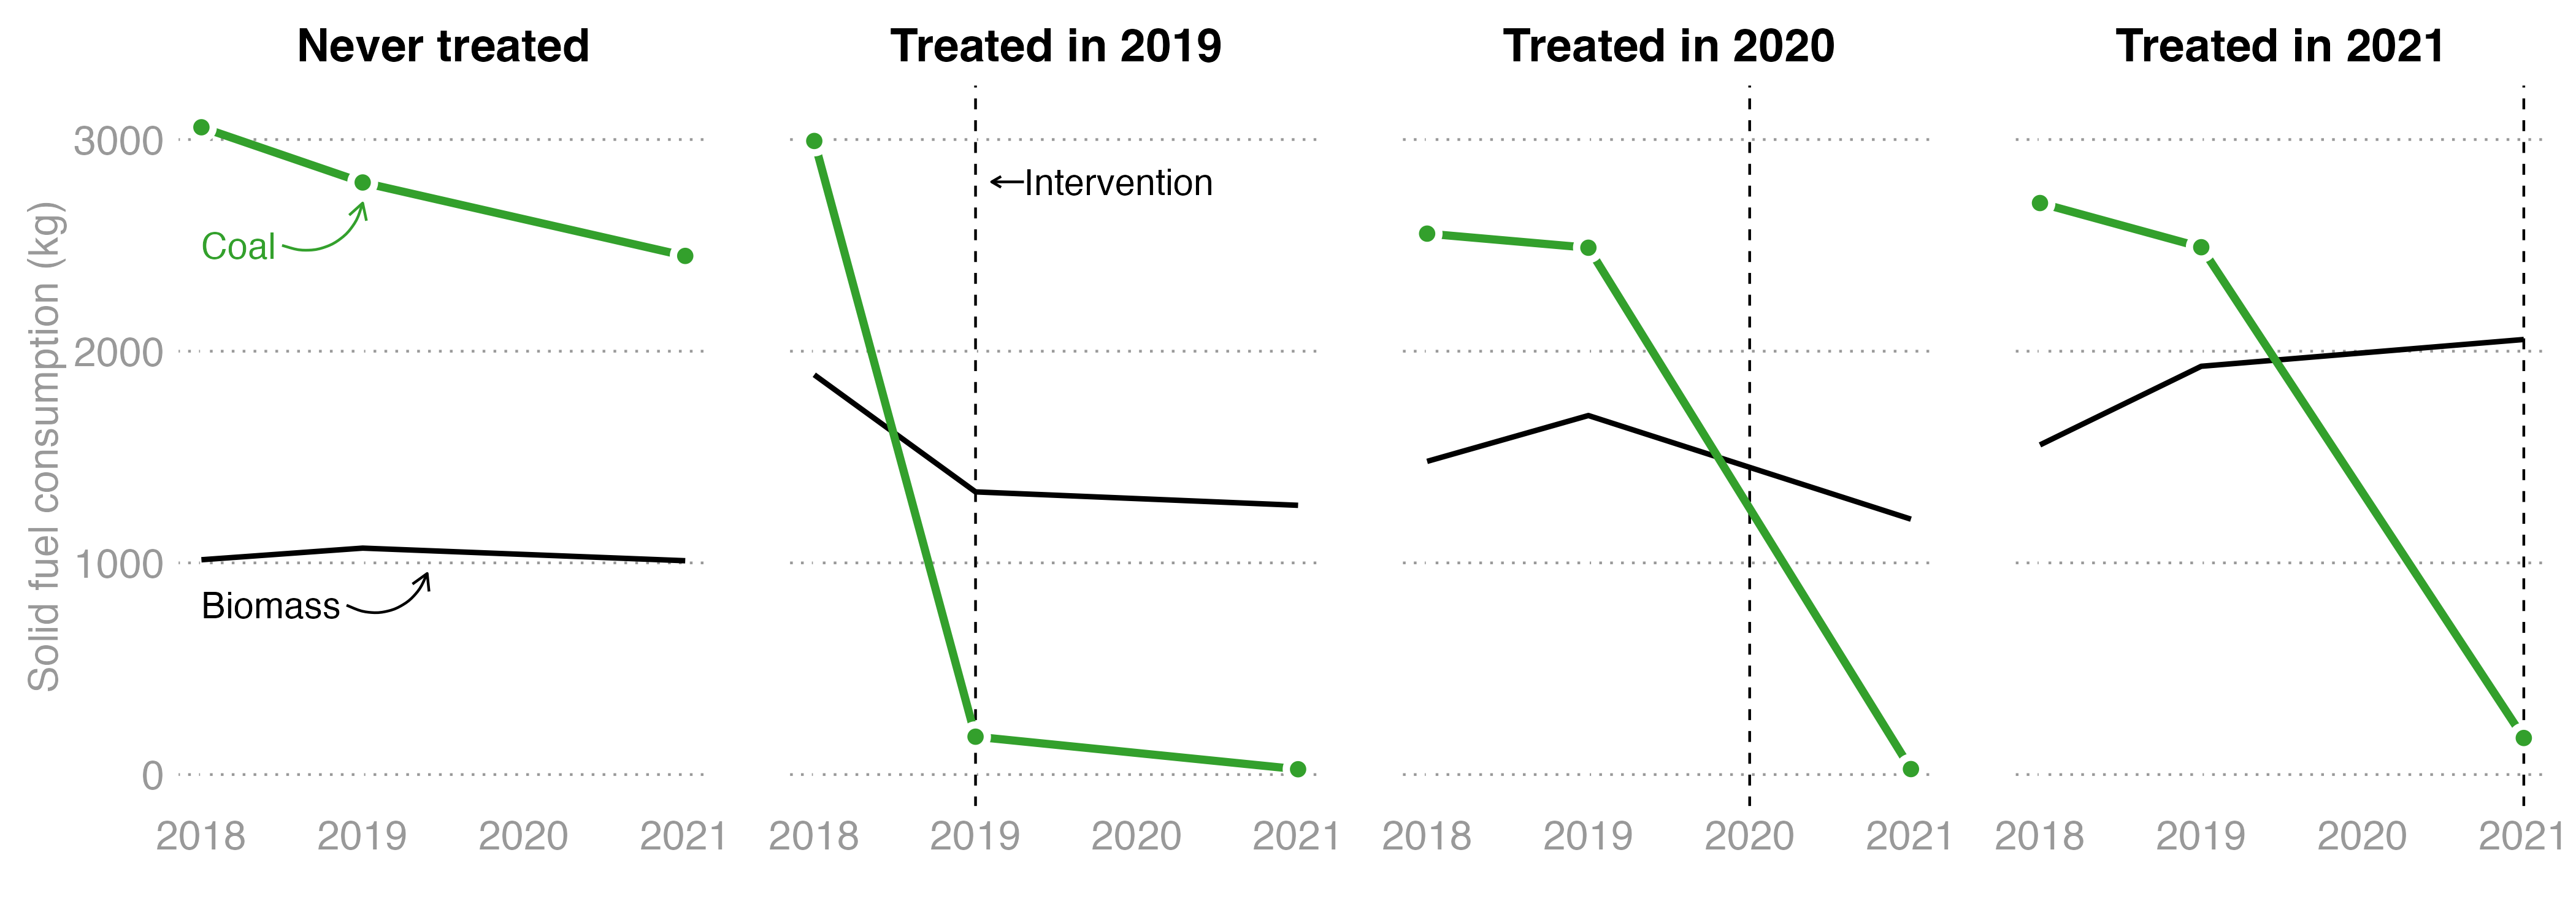
\includegraphics[width=1\textwidth,height=\textheight]{images/coal-plot.png}

}

\caption{\label{fig-afig-coal}Trends in self-reported coal and biomass,
by treatment season}

\end{figure}

\hypertarget{tbl-fuel-did}{}
\begin{table}[H]
\caption{\label{tbl-fuel-did}Policy impacts on self-reported fuel use (kg) }\tabularnewline

\centering
\begin{tabular}{>{\centering\arraybackslash}p{1.5cm}>{\centering\arraybackslash}p{1.5cm}cccc}
\toprule
\multicolumn{2}{c}{ } & \multicolumn{2}{c}{Coal\textsuperscript{a}} & \multicolumn{2}{c}{Biomass\textsuperscript{b}} \\
\cmidrule(l{3pt}r{3pt}){3-4} \cmidrule(l{3pt}r{3pt}){5-6}
Cohort & Time & ATT & (95\%CI) & ATT & (95\%CI)\\
\midrule
\addlinespace[0.3em]
\multicolumn{6}{l}{\textbf{Average ATT}}\\
All & All & -2361 & (-2677, -2044) & -487 & (-805, -168)\\
\addlinespace[0.3em]
\multicolumn{6}{l}{\textbf{Cohort-Time ATTs}}\\
2019 & 2019 & -2631 & (-2913, -2348) & -653 & (-991, -315)\\
2019 & 2021 & -2416 & (-2847, -1984) & -633 & (-1201, -64)\\
2020 & 2021 & -2018 & (-2474, -1562) & -350 & (-701, 0)\\
2021 & 2021 & -1961 & (-2895, -1027) & 338 & (-30, 705)\\
\bottomrule
\multicolumn{6}{l}{\rule{0pt}{1em}\textsuperscript{a} Joint test that all ATTs are equal: F(3, 2886)= 1.856, p= 0.135}\\
\multicolumn{6}{l}{\rule{0pt}{1em}\textsuperscript{b} Joint test that all ATTs are equal: F(3, 2886)= 5.545, p= 0.001}\\
\end{tabular}
\end{table}

Sensitivity analyses: {[}{[}{[}Jill to edit this table include all
sensitivity analysis for total effects models{]}{]}{]}

\begin{verbatim}
Number of participants (observations)
Mean change or percent change in FeNO (ppb)
Limited to participants with two or more measurements
142 (569)
-0.2 [-3.0, 2.5]
Limited to participants with three measurements
95 (285)
0.4 [-2.8, 3.6]
Analysis with log-transformed outcome [ln(FeNO)]
511 (843)
-3.8% [-16.9, 11.4]
\end{verbatim}

\newpage

\hypertarget{heterogeneity-in-treament-effects}{%
\subsection{Heterogeneity in treament
effects}\label{heterogeneity-in-treament-effects}}

\hypertarget{personal-exposure}{%
\subsubsection{Personal exposure}\label{personal-exposure}}

As noted in the methods section\ldots Table
Table~\ref{tbl-a-het-personal} shows limited evidence that the ATTs
across cohorts and time demonstrate meaningful heterogeneity.

\hypertarget{tbl-a-het-personal}{}
\begin{table}[H]
\caption{\label{tbl-a-het-personal}Heterogenous treatment effects: Personal exposures }\tabularnewline

\centering
\begin{tabular}{>{\centering\arraybackslash}p{1.5cm}>{\centering\arraybackslash}p{1.5cm}cccc}
\toprule
\multicolumn{2}{c}{ } & \multicolumn{2}{c}{PM2.5\textsuperscript{a}} & \multicolumn{2}{c}{Black carbon\textsuperscript{b}} \\
\cmidrule(l{3pt}r{3pt}){3-4} \cmidrule(l{3pt}r{3pt}){5-6}
Cohort & Time & ATT & (95\%CI) & ATT & (95\%CI)\\
\midrule
\addlinespace[0.3em]
\multicolumn{6}{l}{\textbf{Average ATT}}\\
All & All & 1.95 & (-23.34, 27.23) & -0.43 & (-1.67, 0.81)\\
\addlinespace[0.3em]
\multicolumn{6}{l}{\textbf{Cohort-Time ATTs}}\\
2019 & 2019 & -0.05 & (-28.97, 28.87) & -0.69 & (-1.84, 0.45)\\
2019 & 2021 & -4.31 & (-41.92, 33.3) & -0.25 & (-2.11, 1.62)\\
2020 & 2021 & 23.61 & (-19.88, 67.11) & -0.27 & (-2.04, 1.5)\\
2021 & 2021 & -19.06 & (-43.19, 5.07) & -0.56 & (-2.46, 1.34)\\
\bottomrule
\multicolumn{6}{l}{\rule{0pt}{1em}\textsuperscript{a} Joint test that all ATTs are equal: F(3, 1271)= 0.431, p= 0.731}\\
\multicolumn{6}{l}{\rule{0pt}{1em}\textsuperscript{b} Joint test that all ATTs are equal: F(3, 1253)= 0.613, p= 0.607}\\
\end{tabular}
\end{table}

\hypertarget{indoor-pm2.5-1}{%
\subsubsection{\texorpdfstring{Indoor
PM\textsubscript{2.5}}{Indoor PM2.5}}\label{indoor-pm2.5-1}}

Table Table~\ref{tbl-a-het-indoor} shows estimates for cohort-time ATTs
for daily and seasonal indoor PM\textsubscript{2.5}.

\hypertarget{tbl-a-het-indoor}{}
\begin{table}[H]
\caption{\label{tbl-a-het-indoor}Heterogenous treatment effects: Indoor }\tabularnewline

\centering
\begin{tabular}{>{\centering\arraybackslash}p{1.5cm}>{\centering\arraybackslash}p{1.5cm}cccc}
\toprule
\multicolumn{2}{c}{ } & \multicolumn{2}{c}{Daily\textsuperscript{a}} & \multicolumn{2}{c}{Seasonal\textsuperscript{b}} \\
\cmidrule(l{3pt}r{3pt}){3-4} \cmidrule(l{3pt}r{3pt}){5-6}
Cohort & Time & ATT & (95\%CI) & ATT & (95\%CI)\\
\midrule
\addlinespace[0.3em]
\multicolumn{6}{l}{\textbf{Average ATT}}\\
All & All & -14.20 & (-53.94, 25.54) & -36.19 & (-60.74, -11.65)\\
\addlinespace[0.3em]
\multicolumn{6}{l}{\textbf{Cohort-Time ATTs}}\\
2020 & 2021 & -4.71 & (-56.93, 47.5) & -25.44 & (-58.02, 7.13)\\
2021 & 2021 & -37.24 & (-74.15, -0.33) & -59.23 & (-79.61, -38.85)\\
\bottomrule
\multicolumn{6}{l}{\rule{0pt}{1em}\textsuperscript{a} Joint test that all ATTs are equal: F(1, 405)= 0.064, p= 0.8}\\
\multicolumn{6}{l}{\rule{0pt}{1em}\textsuperscript{b} Joint test that all ATTs are equal: F(1, 368)= 0.756, p= 0.385}\\
\end{tabular}
\end{table}

\hypertarget{indoor-temperature}{%
\subsubsection{Indoor temperature}\label{indoor-temperature}}

{[}To come\ldots{]}

\hypertarget{blood-pressure-outcomes}{%
\subsubsection{Blood pressure outcomes}\label{blood-pressure-outcomes}}

Table~\ref{tbl-bp-het} shows ATTs by treatment cohort and time, as well
as the results of joint tests of heterogeneity across ATTs.

\hypertarget{tbl-bp-het}{}
\begin{table}
\caption{\label{tbl-bp-het}Heterogenous treatment effects for the total effect of the CBHP policy
on blood pressure. }\tabularnewline

\centering
\begin{threeparttable}
\begin{tabular}{>{\raggedright\arraybackslash}p{2cm}>{\raggedright\arraybackslash}p{2cm}cccc}
\toprule
\multicolumn{2}{c}{ } & \multicolumn{2}{c}{Adjusted DiD\textsuperscript{a}} & \multicolumn{2}{c}{Heterogeneity tests\textsuperscript{b}} \\
\cmidrule(l{3pt}r{3pt}){3-4} \cmidrule(l{3pt}r{3pt}){5-6}
Cohort & Time & ATT & (95\%CI) & F-Statistic & p-value\\
\midrule
\addlinespace[0.3em]
\multicolumn{6}{l}{\textbf{Brachial SBP}}\\
\hspace{1em}2019 & 2019 & -2.36 & (-5.23, 0.5) &  & \\
\hspace{1em}2019 & 2021 & -1.51 & (-4.01, 0.98) &  & \\
\hspace{1em}2020 & 2021 & -1.26 & (-4.97, 2.45) &  & \\
\hspace{1em}2021 & 2021 & 2.39 & (-0.49, 5.28) & 2.3 & 0.080\\
\addlinespace[0.3em]
\multicolumn{6}{l}{\textbf{Central SBP}}\\
\hspace{1em}2019 & 2019 & -2.03 & (-4.69, 0.63) &  & \\
\hspace{1em}2019 & 2021 & -1.96 & (-4.45, 0.52) &  & \\
\hspace{1em}2020 & 2021 & -1.78 & (-5.07, 1.52) &  & \\
\hspace{1em}2021 & 2021 & 2.11 & (-1.09, 5.31) & 1.9 & 0.140\\
\addlinespace[0.3em]
\multicolumn{6}{l}{\textbf{Brachial DBP}}\\
\hspace{1em}2019 & 2019 & -2.66 & (-4.67, -0.65) &  & \\
\hspace{1em}2019 & 2021 & -2.37 & (-4.01, -0.72) &  & \\
\hspace{1em}2020 & 2021 & 0.2 & (-1.54, 1.94) &  & \\
\hspace{1em}2021 & 2021 & 0.78 & (-0.48, 2.05) & 6.8 & 0.000\\
\addlinespace[0.3em]
\multicolumn{6}{l}{\textbf{Central DBP}}\\
\hspace{1em}2019 & 2019 & -2.67 & (-4.57, -0.78) &  & \\
\hspace{1em}2019 & 2021 & -2.55 & (-4.15, -0.94) &  & \\
\hspace{1em}2020 & 2021 & 0.11 & (-1.67, 1.9) &  & \\
\hspace{1em}2021 & 2021 & 1.09 & (-0.06, 2.23) & 10.0 & 0.000\\
\bottomrule
\end{tabular}
\begin{tablenotes}
\item \small{Note: ATT = Average Treatment Effect on the Treated, DiD = Difference-in-Differences, CDE = Controlled Direct Effect.}
\item[a] \small{Adjusted for age, sex, waist circumference, smoking, alcohol consumption, and use of blood pressure medication.}
\item[b] \small{F-statistics and p-values for joint tests of equality across cohort and time ATTs}
\end{tablenotes}
\end{threeparttable}
\end{table}

\hypertarget{mediation-analyses-for-blood-pressure}{%
\subsubsection{Mediation analyses for blood
pressure}\label{mediation-analyses-for-blood-pressure}}

Table~\ref{tbl-a-bp-med-het} shows the cohort-time treatment effects for
the mediation model for blood pressure.

\hypertarget{tbl-a-bp-med-het}{}
\begin{table}[H]
\caption{\label{tbl-a-bp-med-het}Heterogenous treatment effects for blood pressure mediation model }\tabularnewline

\centering\begingroup\fontsize{10}{12}\selectfont

\begin{threeparttable}
\begin{tabular}{llcccccccc}
\toprule
\multicolumn{2}{c}{ } & \multicolumn{2}{c}{Adjusted Total Effect\textsuperscript{a}} & \multicolumn{6}{c}{CDE Mediated By:\textsuperscript{b}} \\
\cmidrule(l{3pt}r{3pt}){3-4} \cmidrule(l{3pt}r{3pt}){5-10}
\multicolumn{4}{c}{ } & \multicolumn{2}{c}{Indoor PM} & \multicolumn{2}{c}{Indoor Temp} & \multicolumn{2}{c}{PM + Temp} \\
\cmidrule(l{3pt}r{3pt}){5-6} \cmidrule(l{3pt}r{3pt}){7-8} \cmidrule(l{3pt}r{3pt}){9-10}
Cohort & Time & ATT & (95\%CI) & ATT & (95\%CI) & ATT & (95\%CI) & ATT & (95\%CI)\\
\midrule
\addlinespace[0.3em]
\multicolumn{10}{l}{\textbf{Brachial SBP}}\\
\hspace{1em}2019 & 2019 & -2.36 & (-5.23, 0.50) & -2.15 & (-5.14, 0.84) & -1.69 & (-4.54, 1.15) & -1.24 & (-4.20, 1.72)\\
\hspace{1em}2019 & 2021 & -1.51 & (-4.01, 0.98) & -1.27 & (-4.01, 1.47) & -0.41 & (-2.92, 2.10) & 0.01 & (-2.71, 2.74)\\
\hspace{1em}2020 & 2021 & -1.26 & (-4.97, 2.45) & -0.54 & (-4.25, 3.17) & 0.43 & (-2.86, 3.73) & 1.04 & (-2.59, 4.67)\\
\hspace{1em}2021 & 2021 & 2.39 & (-0.49, 5.28) & 2.68 & (-0.42, 5.79) & 1.95 & (-1.74, 5.64) & 1.88 & (-1.92, 5.67)\\
\addlinespace[0.3em]
\multicolumn{10}{l}{\textbf{Central SBP}}\\
\hspace{1em}2019 & 2019 & -2.03 & (-4.69, 0.63) & -1.75 & (-4.61, 1.11) & -1.40 & (-4.06, 1.27) & -0.89 & (-3.73, 1.95)\\
\hspace{1em}2019 & 2021 & -1.96 & (-4.45, 0.52) & -1.65 & (-4.40, 1.11) & -0.93 & (-3.18, 1.32) & -0.44 & (-2.95, 2.07)\\
\hspace{1em}2020 & 2021 & -1.78 & (-5.07, 1.52) & -1.00 & (-4.36, 2.36) & -0.15 & (-3.18, 2.88) & 0.47 & (-2.95, 3.89)\\
\hspace{1em}2021 & 2021 & 2.11 & (-1.09, 5.31) & 2.45 & (-0.83, 5.73) & 1.66 & (-1.73, 5.05) & 1.63 & (-1.82, 5.08)\\
\addlinespace[0.3em]
\multicolumn{10}{l}{\textbf{Brachial DBP}}\\
\hspace{1em}2019 & 2019 & -2.66 & (-4.67, -0.65) & -2.47 & (-4.70, -0.25) & -2.29 & (-4.18, -0.40) & -1.94 & (-4.03, 0.14)\\
\hspace{1em}2019 & 2021 & -2.37 & (-4.01, -0.72) & -2.10 & (-4.09, -0.11) & -1.81 & (-3.21, -0.41) & -1.50 & (-3.28, 0.27)\\
\hspace{1em}2020 & 2021 & 0.20 & (-1.54, 1.94) & 0.31 & (-1.43, 2.04) & 1.14 & (-0.65, 2.94) & 1.23 & (-0.70, 3.15)\\
\hspace{1em}2021 & 2021 & 0.78 & (-0.48, 2.05) & 1.05 & (-0.59, 2.69) & 0.20 & (-1.21, 1.62) & 0.36 & (-1.34, 2.06)\\
\addlinespace[0.3em]
\multicolumn{10}{l}{\textbf{Central DBP}}\\
\hspace{1em}2019 & 2019 & -2.67 & (-4.57, -0.78) & -2.43 & (-4.58, -0.28) & -2.52 & (-4.34, -0.70) & -2.13 & (-4.18, -0.08)\\
\hspace{1em}2019 & 2021 & -2.55 & (-4.15, -0.94) & -2.20 & (-4.18, -0.22) & -2.18 & (-3.60, -0.76) & -1.80 & (-3.58, -0.03)\\
\hspace{1em}2020 & 2021 & 0.11 & (-1.67, 1.90) & 0.22 & (-1.58, 2.01) & 1.07 & (-0.74, 2.87) & 1.16 & (-0.80, 3.13)\\
\hspace{1em}2021 & 2021 & 1.09 & (-0.06, 2.23) & 1.39 & (-0.16, 2.94) & 0.51 & (-0.80, 1.82) & 0.70 & (-0.94, 2.34)\\
\bottomrule
\end{tabular}
\begin{tablenotes}
\item \small{Note: Results combined across 30 multiply-imputed datasets. ATT = Average Treatment Effect on the Treated, CDE = Controlled Direct Effect, DBP = Diastolic blood pressure, SBP = Systolic blood pressure.}
\item[a] \small{Adjusted for age, sex, waist circumference, smoking, alcohol consumption, and use of blood pressure medication.}
\item[b] \small{Mediators were set to the mean value for untreated participants at baseline.}
\end{tablenotes}
\end{threeparttable}
\endgroup{}
\end{table}

\hypertarget{tbl-a-bp-med-het-tests}{}
\begin{table}
\caption{\label{tbl-a-bp-med-het-tests}Heterogenous treatment effects and tests for cohort-time heterogeneity
across CDEs for multiple mediation blood pressure mediation model. }\tabularnewline

\centering
\begin{threeparttable}
\begin{tabular}{>{\raggedright\arraybackslash}p{2cm}>{\raggedright\arraybackslash}p{2cm}cccc}
\toprule
\multicolumn{2}{c}{ } & \multicolumn{2}{c}{Adjusted CDE\textsuperscript{a}} & \multicolumn{2}{c}{Heterogeneity tests\textsuperscript{b}} \\
\cmidrule(l{3pt}r{3pt}){3-4} \cmidrule(l{3pt}r{3pt}){5-6}
Cohort & Time & ATT & (95\%CI) & F-Statistic & p-value\\
\midrule
\addlinespace[0.3em]
\multicolumn{6}{l}{\textbf{Brachial SBP}}\\
\hspace{1em}2019 & 2019 & -1.24 & (-4.20, 1.72) &  & \\
\hspace{1em}2019 & 2021 & 0.01 & (-2.71, 2.74) &  & \\
\hspace{1em}2020 & 2021 & 1.04 & (-2.59, 4.67) &  & \\
\hspace{1em}2021 & 2021 & 1.88 & (-1.92, 5.67) & 0.8 & 0.513\\
\addlinespace[0.3em]
\multicolumn{6}{l}{\textbf{Central SBP}}\\
\hspace{1em}2019 & 2019 & -0.89 & (-3.73, 1.95) &  & \\
\hspace{1em}2019 & 2021 & -0.44 & (-2.95, 2.07) &  & \\
\hspace{1em}2020 & 2021 & 0.47 & (-2.95, 3.89) &  & \\
\hspace{1em}2021 & 2021 & 1.63 & (-1.82, 5.08) & 0.6 & 0.608\\
\addlinespace[0.3em]
\multicolumn{6}{l}{\textbf{Brachial DBP}}\\
\hspace{1em}2019 & 2019 & -1.94 & (-4.03, 0.14) &  & \\
\hspace{1em}2019 & 2021 & -1.50 & (-3.28, 0.27) &  & \\
\hspace{1em}2020 & 2021 & 1.23 & (-0.70, 3.15) &  & \\
\hspace{1em}2021 & 2021 & 0.36 & (-1.34, 2.06) & 3.9 & 0.008\\
\addlinespace[0.3em]
\multicolumn{6}{l}{\textbf{Central DBP}}\\
\hspace{1em}2019 & 2019 & -2.13 & (-4.18, -0.08) &  & \\
\hspace{1em}2019 & 2021 & -1.80 & (-3.58, -0.03) &  & \\
\hspace{1em}2020 & 2021 & 1.16 & (-0.80, 3.13) &  & \\
\hspace{1em}2021 & 2021 & 0.70 & (-0.94, 2.34) & 4.8 & 0.003\\
\bottomrule
\end{tabular}
\begin{tablenotes}
\item \small{Note: ATT = Average Treatment Effect on the Treated, DiD = Difference-in-Differences, CDE = Controlled Direct Effect.}
\item[a] \small{Adjusted for age, sex, waist circumference, smoking, alcohol consumption, and use of blood pressure medication.}
\item[b] \small{F-statistics and p-values for joint tests of equality across cohort and time ATTs}
\end{tablenotes}
\end{threeparttable}
\end{table}

\newpage

\hypertarget{respiratory-outcomes}{%
\subsubsection{Respiratory outcomes}\label{respiratory-outcomes}}

Appendix tables \ref{tbl-a-het-resp}, \ref{tbl-a-het-cough},
\ref{tbl-a-het-phlegm}, \ref{tbl-a-het-wheeze}, \ref{tbl-a-het-breath},
\ref{tbl-a-het-nochest} below show Average Treatment Effect on the
Treated (ATTs) by treatment cohort and time. ATTs are derived from
estimating marginal effects from extended two-way fixed effects models
with additional adjustment for age, sex, and smoking status.

\hypertarget{tbl-a-het-resp}{}
\begin{table}
\caption{\label{tbl-a-het-resp}Heterogenous treatment effects for self-reported respiratory outcomes:
Any respiratory symptom }\tabularnewline

\centering
\begin{tabular}{>{\centering\arraybackslash}p{2cm}>{\centering\arraybackslash}p{2cm}cc}
\toprule
Cohort & Time & ATT & (95\%CI)\\
\midrule
\addlinespace[0.3em]
\multicolumn{4}{l}{\textbf{Average ATT}}\\
All & All & -0.08 & (-0.15, -0.01)\\
\addlinespace[0.3em]
\multicolumn{4}{l}{\textbf{Cohort-Time ATTs}}\\
2019 & 2019 & -0.11 & (-0.20, -0.02)\\
2019 & 2021 & -0.10 & (-0.21, 0.00)\\
2020 & 2021 & 0.01 & (-0.10, 0.13)\\
2021 & 2021 & -0.12 & (-0.22, -0.01)\\
\bottomrule
\multicolumn{4}{l}{\rule{0pt}{1em}\small{Note: Joint test that all ATTs are equal: F(3, 2579)= 1.283, p= 0.278.}}\\
\end{tabular}
\end{table}

\hypertarget{tbl-a-het-cough}{}
\begin{table}
\caption{\label{tbl-a-het-cough}Heterogenous treatment effects for self-reported respiratory outcomes:
Coughing }\tabularnewline

\centering
\begin{tabular}{>{\centering\arraybackslash}p{2cm}>{\centering\arraybackslash}p{2cm}cc}
\toprule
Cohort & Time & ATT & (95\%CI)\\
\midrule
\addlinespace[0.3em]
\multicolumn{4}{l}{\textbf{Average ATT}}\\
All & All & -0.02 & (-0.07, 0.03)\\
\addlinespace[0.3em]
\multicolumn{4}{l}{\textbf{Cohort-Time ATTs}}\\
2019 & 2019 & -0.04 & (-0.11, 0.03)\\
2019 & 2021 & 0.01 & (-0.07, 0.08)\\
2020 & 2021 & -0.03 & (-0.10, 0.05)\\
2021 & 2021 & -0.04 & (-0.09, 0.02)\\
\bottomrule
\multicolumn{4}{l}{\rule{0pt}{1em}\small{Note: Joint test that all ATTs are equal: F(3, 2579)= 0.732, p= 0.533.}}\\
\end{tabular}
\end{table}

\hypertarget{tbl-a-het-phlegm}{}
\begin{table}
\caption{\label{tbl-a-het-phlegm}Heterogenous treatment effects for self-reported respiratory outcomes:
Phlegm }\tabularnewline

\centering
\begin{tabular}{>{\centering\arraybackslash}p{2cm}>{\centering\arraybackslash}p{2cm}cc}
\toprule
Cohort & Time & ATT & (95\%CI)\\
\midrule
\addlinespace[0.3em]
\multicolumn{4}{l}{\textbf{Average ATT}}\\
All & All & -0.02 & (-0.06, 0.03)\\
\addlinespace[0.3em]
\multicolumn{4}{l}{\textbf{Cohort-Time ATTs}}\\
2019 & 2019 & -0.06 & (-0.16, 0.03)\\
2019 & 2021 & -0.03 & (-0.10, 0.04)\\
2020 & 2021 & 0.04 & (-0.02, 0.09)\\
2021 & 2021 & 0.03 & (-0.04, 0.09)\\
\bottomrule
\multicolumn{4}{l}{\rule{0pt}{1em}\small{Note: Joint test that all ATTs are equal: F(3, 2579)= 1.735, p= 0.158.}}\\
\end{tabular}
\end{table}

\hypertarget{tbl-a-het-wheeze}{}
\begin{table}
\caption{\label{tbl-a-het-wheeze}Heterogenous treatment effects for self-reported respiratory outcomes:
Wheezing attacks }\tabularnewline

\centering
\begin{tabular}{>{\centering\arraybackslash}p{2cm}>{\centering\arraybackslash}p{2cm}cc}
\toprule
Cohort & Time & ATT & (95\%CI)\\
\midrule
\addlinespace[0.3em]
\multicolumn{4}{l}{\textbf{Average ATT}}\\
All & All & 0.00 & (-0.04, 0.04)\\
\addlinespace[0.3em]
\multicolumn{4}{l}{\textbf{Cohort-Time ATTs}}\\
2019 & 2019 & -0.02 & (-0.06, 0.01)\\
2019 & 2021 & 0.01 & (-0.04, 0.06)\\
2020 & 2021 & -0.03 & (-0.11, 0.05)\\
2021 & 2021 & 0.09 & (-0.00, 0.18)\\
\bottomrule
\multicolumn{4}{l}{\rule{0pt}{1em}\small{Note: Joint test that all ATTs are equal: F(3, 2579)= 2.923, p= 0.033.}}\\
\end{tabular}
\end{table}

\hypertarget{tbl-a-het-breath}{}
\begin{table}
\caption{\label{tbl-a-het-breath}Heterogenous treatment effects for self-reported respiratory outcomes:
Trouble breathing }\tabularnewline

\centering
\begin{tabular}{>{\centering\arraybackslash}p{2cm}>{\centering\arraybackslash}p{2cm}cc}
\toprule
Cohort & Time & ATT & (95\%CI)\\
\midrule
\addlinespace[0.3em]
\multicolumn{4}{l}{\textbf{Average ATT}}\\
All & All & -0.05 & (-0.12, 0.02)\\
\addlinespace[0.3em]
\multicolumn{4}{l}{\textbf{Cohort-Time ATTs}}\\
2019 & 2019 & -0.06 & (-0.16, 0.04)\\
2019 & 2021 & -0.07 & (-0.16, 0.03)\\
2020 & 2021 & 0.01 & (-0.09, 0.11)\\
2021 & 2021 & -0.07 & (-0.20, 0.06)\\
\bottomrule
\multicolumn{4}{l}{\rule{0pt}{1em}\small{Note: Joint test that all ATTs are equal: F(3, 2579)= 0.718, p= 0.541.}}\\
\end{tabular}
\end{table}

\hypertarget{tbl-a-het-nochest}{}
\begin{table}
\caption{\label{tbl-a-het-nochest}Heterogenous treatment effects for self-reported respiratory outcomes:
Chest trouble }\tabularnewline

\centering
\begin{tabular}{>{\centering\arraybackslash}p{2cm}>{\centering\arraybackslash}p{2cm}cc}
\toprule
Cohort & Time & ATT & (95\%CI)\\
\midrule
\addlinespace[0.3em]
\multicolumn{4}{l}{\textbf{Average ATT}}\\
All & All & -0.06 & (-0.12, -0.01)\\
\addlinespace[0.3em]
\multicolumn{4}{l}{\textbf{Cohort-Time ATTs}}\\
2019 & 2019 & -0.06 & (-0.13, 0.01)\\
2019 & 2021 & -0.06 & (-0.15, 0.03)\\
2020 & 2021 & -0.05 & (-0.16, 0.05)\\
2021 & 2021 & -0.14 & (-0.22, -0.05)\\
\bottomrule
\multicolumn{4}{l}{\rule{0pt}{1em}\small{Note: Joint test that all ATTs are equal: F(3, 2579)= 1.046, p= 0.371.}}\\
\end{tabular}
\end{table}

\hypertarget{outdoor-and-personal-mixed-combustion}{%
\subsubsection{Outdoor and personal mixed
combustion}\label{outdoor-and-personal-mixed-combustion}}

\begin{figure}[H]

{\centering 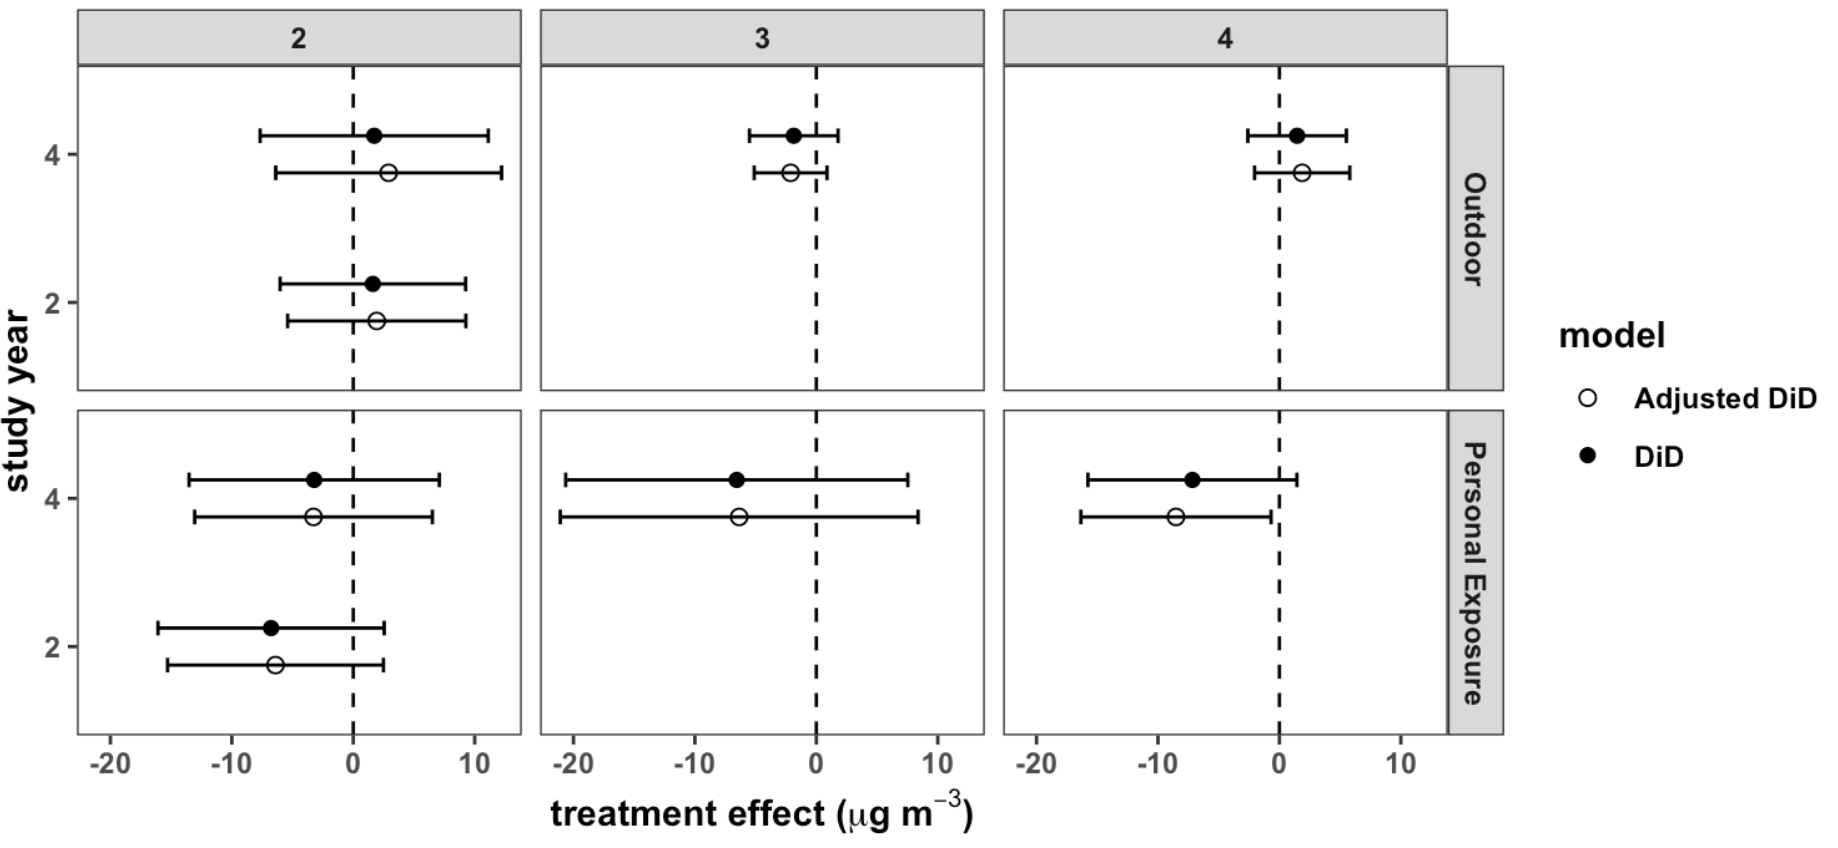
\includegraphics[width=1\textwidth,height=\textheight]{images/did-mixed-ct.png}

}

\caption{\label{fig-afig-mixed-ct}Adjusted and unadjusted treatment
effect for outdoor and personal exposure (µg/m\textsuperscript{3}) to
the mixed combustion source by treatment year.}

\end{figure}

\hypertarget{impact-of-including-season-3-data}{%
\subsection{Impact of including Season 3
data}\label{impact-of-including-season-3-data}}

Table~\ref{tbl-a-ind-s3} shows differences in the ATTs for the impact of
seasonal indoor PM\textsubscript{2.5} when season 3 data (collected in
41 villages during COVID-19) are included versus excluded.

\hypertarget{tbl-a-ind-s3}{}
\begin{table}
\caption{\label{tbl-a-ind-s3}Effects of the CBHP policy on indoor seasonal PM\textsubscript{2.5}
based on whether Season 3 data are included vs.~excluded. }\tabularnewline

\centering
\begin{tabular}{>{\centering\arraybackslash}p{1.5cm}>{\centering\arraybackslash}p{1.5cm}cccc}
\toprule
\multicolumn{2}{c}{ } & \multicolumn{2}{c}{With Season 3 data} & \multicolumn{2}{c}{Without Season 3 data} \\
\cmidrule(l{3pt}r{3pt}){3-4} \cmidrule(l{3pt}r{3pt}){5-6}
Cohort & Time & ATT & (95\%CI) & ATT & (95\%CI)\\
\midrule
\addlinespace[0.3em]
\multicolumn{6}{l}{\textbf{Average ATT}}\\
All & All & -37.49 & (-60.11, -14.88) & -35.11 & (-59.36, -10.85)\\
\addlinespace[0.3em]
\multicolumn{6}{l}{\textbf{Cohort-Time ATTs}}\\
2020 & 2020 & -36.94 & (-61.39, -12.49) & 0.00 & (NA, NA)\\
2020 & 2021 & -33.51 & (-66.84, -0.18) & -30.22 & (-63.77, 3.32)\\
2021 & 2021 & -46.82 & (-58.57, -35.07) & -44.88 & (-60.41, -29.34)\\
\bottomrule
\multicolumn{6}{l}{\rule{0pt}{1em}\textit{Note: }}\\
\multicolumn{6}{l}{\rule{0pt}{1em}Sample sizes for}\\
\end{tabular}
\end{table}

\hypertarget{about-the-authors}{%
\section*{About the authors}\label{about-the-authors}}
\addcontentsline{toc}{section}{About the authors}

\hypertarget{other-publications}{%
\section*{Other publications}\label{other-publications}}
\addcontentsline{toc}{section}{Other publications}

Li X, Baumgartner J, Barrington-Leigh C, Harper S, Robinson B, Shen G,
et al.~2022a. Socioeconomic and Demographic Associations with Wintertime
Air Pollution Exposures at Household, Community, and District Scales in
Rural Beijing, China. Environ Sci Technol 56:8308--8318;
doi:10.1021/acs.est.1c07402.

Li X, Baumgartner J, Harper S, Zhang X, Sternbach T, Barrington-Leigh C,
et al.~2022b. Field measurements of indoor and community air quality in
rural Beijing before, during, and after the COVID-19 lockdown. Indoor
Air 32:e13095; doi:10.1111/ina.13095.

Sternbach TJ, Harper S, Li X, Zhang X, Carter E, Zhang Y, et al.~2022.
Effects of indoor and outdoor temperatures on blood pressure and central
hemodynamics in a wintertime longitudinal study of Chinese adults. J
Hypertension 40:1950--1959; doi:10.1097/HJH.0000000000003198.

{[}a{]}Updated PDF here:
https://github.com/sbh4th/bhet-report/blob/main/hei-report.pdf
{[}b{]}could potentially move elsewhere.
{[}c{]}(\textbf{talia.sternbach?})(\textbf{gmail.com?})
(\textbf{xiaoyingcsu?})(\textbf{gmail.com?})
(\textbf{ellison.carter?})(\textbf{gmail.com?})

When I look at this picture, all I think about is transporting all of
those sensors and cords across the rooftop and down multiple flights of
stairs --- only to be met with a locked door separating us from the
driver \ldots{} and the student with the key was nowhere to be found.
{[}d{]}\#thelivedexperiencereport {[}e{]}haha! Or when we sorted through
supplies in the 110 degree heat and in that gross/dirty/polluted attic
at Tsinghua? {[}f{]}Oh goodness. That is an old memory. Probably my most
elevated acute VOC exposure to date. Thankfully, neither of us fell down
the stairs. Still, I think, on some days, I'd trade slogging through
administrative obstacle courses for slogging through attics with the
best fieldwork teammates ever. {[}g{]}hahaha\ldots{} and sled-pushing
all the boxes down the hallway looking for an open door {[}h{]}Yes!!! I
forgot about that. The poor driver was so patient about the key problem
and kept trying to make friendly conversation \ldots{} and we were all
just totally exhausted and hungry.
{[}i{]}(\textbf{jill.baumgartner?})(\textbf{gmail.com?})
(\textbf{jill.baumgartner?})(\textbf{mcgill.ca?})
(\textbf{sam.harper?})(\textbf{mcgill.ca?})

Is the plan to keep this as a separate section or should I be looking
through the discussion for places to put some of these ideas? {[}j{]}For
now the plan is to keep separate sub-headings. {[}k{]}Ok, thanks. Then,
I'll keep working in this section to improve the organization, points
made, citations / refs, and clarity of argument. {[}l{]}I can address by
Wednesday. {[}m{]}(\textbf{ellison.carter?})(\textbf{gmail.com?}). maybe
this is a good place to bring low-cost sensors into the conversation?
Our study would not have been feasible without these. {[}n{]}Good idea.
I'll come back to this on Wednesday.
{[}o{]}(\textbf{ellison.carter?})(\textbf{gmail.com?}). Is it a
measurement problem (too short duration for a highly variable exposure)
or did it not reduce exposure? The group-time models indicate a
consistent 10 ug/m3 reduction in PM2.5 but they are imprecise (except
for the last cohort). {[}p{]}I might have to come back to this. I can't
yet think of an immediate way to fix the discussion to address this
issue.

Two of the three group-time estimates show a statistically imprecise 10
ug/m3 reduction in personal PM, but one group-time estimate doesn't.
Maybe that's enough to say it looks like the intervention worked?

But then, the interpretation becomes one about the statistical
imprecision of the measurement. In past work, by us and others, the
sample sizes have been smaller, so it has seemed more reasonable to say
something about how observing statistical imprecision points to a need
for more, better, longer measurements. But, I'm reluctant to draw that
conclusion here. I honestly don't think a wise outcome of this study is
to say we need more, larger studies measuring air pollution to evaluate
intervention effectiveness. The potential benefits of striving for more
statistically precise estimates of intervention effectiveness don't seem
to outweigh the costs.

In the end, I think there's SUPER modest evidence that the intervention
worked (and a strong rationale that it should have lowered personal
exposure -- coal use effectively ceased). That we didn't observe a a
stronger, more statistically precise measure of treatment effect is too
bad, but I really don't want to interpret this to mean others should do
more measurements for longer in a larger number of people. That's a bias
I am having a tough time overcoming. I'll try to work on this section
more -- if you intend to keep it in the discussion -- and try to write
something. {[}q{]}These results = impact of the policy on ``point''
temperature, measured during HH visits in the 5-min before BP. This is
the temperature mediator in the mediation analysis. Shows different
cohort-time effects for cohort 4-year 4 compared with long-term
temperature cohort-time effects. The 95\% CI for the point-temp does
include the long-term mean indoor temp, though.
(\textbf{jillbaumgartner?})(\textbf{gmail.com?})

xlsx for these results are here: https://osf.io/7wvra



\end{document}
